\documentclass[12pt]{article}
\usepackage{geometry}                % See geometry.pdf to learn the layout options. There are lots.
\geometry{a4paper}                   % ... or a4paper or a5paper or ... 
%\geometry{landscape}                % Activate for for rotated page geometry
%\usepackage[parfill]{parskip}    % Activate to begin paragraphs with an empty line rather than an indent
\usepackage{graphicx}
\usepackage{amssymb}
\usepackage{epstopdf}
\usepackage{caption}
\usepackage{subcaption}
\usepackage[english]{babel}
\usepackage[T1]{fontenc}
\usepackage{epstopdf}
\usepackage[utf8]{inputenc}
\usepackage{units}
\usepackage[toc,page]{appendix}
\usepackage[section]{placeins}
%\usepackage{titling}
\usepackage{cite}
\usepackage{nicefrac}
\usepackage{xcolor}

\usepackage{hyperref}
\usepackage{url}
\newcommand{\subtitle}[1]{%
  \posttitle{%
    \par\end{center}
    \begin{center}\large#1\end{center}
    \vskip0.5em}%
}
\RequirePackage{lineno}
\setlength{\linenumbersep}{6pt}
\linenumbers

%\title{Jet quenching in fluctuating events in heavy-ion collisions}
%\title{Particle Identified Flow and Unfolding in Heavy Ion Collisions}
%\subtitle{Master's thesis}
%\author{Tomas Snellman}
%\date{}                                           % Activate to display a given date or no date


\def\fig#1{Fig.~\ref{#1}}
\def\eq#1{Eq.~(\ref{#1})}
\def\tab#1{Tab.~\ref{#1}}
\def\sec#1{Sec.~\ref{#1}}

\def\tev{\mbox{~TeV}}
\def\gevc{\mbox{~GeV/$c$}}
\def\gevcc{\mbox{~GeV/$c^2$}}
\def\mevc{\mbox{~MeV/$c$}}

\def\simge{\stackrel{>}{\sim} }
\def\simle{\stackrel{<}{\sim} }
%\def\la{\langle }
%\def\ra{\rangle }
\def\la{\left< }
\def\ra{\right> }
\def\mean#1{\ensuremath{\la#1\ra}}
\def\meanabs#1{\ensuremath{\la|#1|\ra}}
\def\meankv#1{\ensuremath{\la#1^2\ra}}
\def\rms#1{\meankv{#1}}
\def\sqrtrms#1{\ensuremath{\sqrt{\meankv{#1}}}}

\def\eg{{\it e.g.}}
\def\etc{{\it etc}}



\newcommand{\sqrtS}{\ensuremath{\sqrt{s}}}
\newcommand{\sqrtSnn}{\ensuremath{\sqrt{s_{\mathrm{NN}}}}}
\newcommand{\sqrtSE}[2][TeV]{\ensuremath{\sqrtS = #2~\mathrm{#1}}}
\newcommand{\sqrtSnnE}[2][TeV]{\ensuremath{\sqrtSnn = #2~\mathrm{#1}}}
\newcommand{\GeVc}{\ensuremath{\mathrm{GeV}\kern-0.05em/\kern-0.02em c}}
\newcommand{\gev}{\ensuremath{\mathrm{GeV}\kern-0.05em}}
\def\pt#1{\ensuremath{p_{\rm T#1}}} 
\def\jt#1{\ensuremath{j_{\rm T#1}}}
\def\vjt#1{\ensuremath{\vec{j}_{\rm T#1}}}
\def\kt#1{\ensuremath{k_{\rm T#1}}}
\newcommand{\xlong} {\ensuremath{x_{\parallel}}}
\def\mean#1{\left<#1\right>}
\def\rms#1{\ensuremath{\sqrt{\left<#1^2\right>}}}
\DeclareUnicodeCharacter{00A0}{ }



\newcommand{\sign} {\ensuremath{\sigma_{\rm N}}}
\newcommand{\siga} {\ensuremath{\sigma_{\rm A}}}
\newcommand{\yn} {\ensuremath{Y_{\rm N}}}
\newcommand{\yf} {\ensuremath{Y_{\rm F}}}
\newcommand{\cf}{\ensuremath{CF}}
\newcommand{\D} {\ensuremath{D^q_\pi}}
\newcommand{\Dz} {\ensuremath{D^h_q(z,Q^2)}}
\newcommand{\fq}{\ensuremath{f_Q(\hat{p}_T)}}
\newcommand{\sq}{\ensuremath{\Sigma_Q(\hat{p}_T)}}
\newcommand{\fkt}{\ensuremath{f^\prime_Q(\hat{p}_{\rm Tt})}}
\newcommand{\skt}{\ensuremath{\Sigma^\prime_Q(\hat{p}_{\rm Tt})}}
\newcommand{\prob}{\ensuremath{\mathcal{P}}}
\newcommand{\condta}{\ensuremath{\Big|_{\pt{t},\pt{a}}}}

\newcommand{\auau} {\ensuremath{Au+Au}}
\newcommand{\dau} {\ensuremath{d+Au}}
\newcommand{\pp}{\ensuremath{\mbox{p\kern-0.05em p}}}
\newcommand{\ppbar}{\ensuremath{\mathrm{p\kern-0.05em \bar{p}}}}
\newcommand{\ee} {\ensuremath{e^+ + e^-}}
\newcommand{\pbpb} {\ensuremath{Pb+Pb}}
\newcommand{\ppb} {\ensuremath{p+Pb}}
\newcommand{\pPb}{\ensuremath{\mbox{p--Pb}}}
\newcommand{\PbPb}{\ensuremath{\mbox{Pb--Pb}}}


\def\ptq#1{\ensuremath{\hat{p}_{\rm T#1}}} 
\def\ptqkv#1{\ensuremath{\hat{p}^2_{\rm T#1}}} 
\def\vptq#1{\ensuremath{\vec{\hat{p}}_{\rm T#1}}} 
\def\ptg{\ensuremath{p_{\rm T\gamma}}} 

\def\pt#1{\ensuremath{p_{\rm T#1}}} 
\def\ptkv#1{\ensuremath{p^2_{\rm T#1}}} 
\def\vpt#1{\ensuremath{\vec{p}_{\rm T#1}}} 

\def\kt#1{\ensuremath{k_{\rm T#1}}} 
\def\ktkv#1{\ensuremath{k^2_{\rm T#1}}} 
\def\vkt#1{\ensuremath{\vec{k}_{\rm T#1}}} 

\def\jt#1{\ensuremath{j_{\rm T#1}}} 
\def\jtkv#1{\ensuremath{j^2_{\rm T#1}}} 
\def\vjt#1{\ensuremath{\vec{j}_{\rm T#1}}} 

\def\mkv#1{\ensuremath{m^2_{#1}}}
\def\mt#1{\ensuremath{m_{\rm T#1}}}
\def\mtkv#1{\ensuremath{m^2_{\rm T#1}}}

\newcommand{\mpt} {\mean{\pt{}}} 
\newcommand{\ptt}{\ensuremath{p_{\rm Tt}}}
\newcommand{\mptt} {\mean{\ptt}} 
\newcommand{\pta}{\ensuremath{p_{\rm Ta}}}
\newcommand{\mpta} {\mean{\pta}} 
\def\pn{\ensuremath{\hat{p}_{\rm n}}} 
\def\pnkv{\ensuremath{\hat{p}^2_{\rm n}}} 
\def\vpn{\ensuremath{\vec{\hat{p}}_{\rm n}}} 

\newcommand{\pout} {\ensuremath{p_{\rm out}}}
\newcommand{\qout} {\ensuremath{\hat{p}_{\rm out}}}


\newcommand{\mz} {\mean{z}}
\newcommand{\zt} {\ensuremath{z_{\rm t}}}
\newcommand{\mzt} {\mean{\zt}}
\newcommand{\za} {\ensuremath{z_{\rm a}}}
\newcommand{\mza} {\mean{\za}}
\newcommand{\xe} {\ensuremath{x_{\rm E}}}
\newcommand{\xh} {\ensuremath{x_{\rm h}}}
\newcommand{\xhq} {\ensuremath{\hat{x}_{\rm h}}}
\newcommand{\zkt} {\ensuremath{ \mean{\zt}\sqrtrms{\kt{}} }}
\newcommand{\xzkt} {\ensuremath{ \xhq^{-1}\mean{\zt}\sqrtrms{\kt{}} }}
\newcommand{\xzktfull} {\ensuremath{ \xhq^{-1}(\kt{},\xh)\mean{\zt(\kt{},\xh)}\sqrtrms{\kt{}} }}

\newcommand{\zT} {\ensuremath{z_{\rm T}}}

\newcommand{\snn} {\ensuremath{\sqrt{s_{NN}}}}
\newcommand{\s} {\ensuremath{\sqrt{s}}}
\newcommand{\piz} {\ensuremath{\pi^0}}
\newcommand{\pizh}{\ensuremath{\pi^0-h^\pm}}
\newcommand{\gammah}{\ensuremath{\rm direct-\gamma-h^\pm}}
\newcommand{\pipmh}{\ensuremath{\pi^\pm-h^\pm}}
\newcommand{\hh}{\ensuremath{h^\pm-h^\pm}}

\newcommand{\pbar} {\ensuremath{\overline{p}}}
\newcommand{\lbar} {\ensuremath{\overline{\Lambda}}}
\newcommand{\ntrig} {\ensuremath{N_{\rm trig}}}
\newcommand{\npart} {\ensuremath{N_{\rm part}}}
\newcommand{\npartav} {\ensuremath{\la N_{\rm part} \ra}}
\newcommand{\ncoll} {\ensuremath{N_{\rm coll}}}
\newcommand{\ncollav} {\ensuremath{\la N_{\rm coll} \ra}}
\newcommand{\ut} {\ensuremath{\la u_t \ra}}

\newcommand{\alphas} {\ensuremath{\alpha_{s}}}
\newcommand{\alphasQ} {\ensuremath{\alpha_{s}(Q^2)}}
\newcommand{\alphasQsqr} {\ensuremath{\alpha_{s}^2(Q^2)}}
\newcommand{\alphaqedQ} {\ensuremath{\alpha_{EM}(Q^2)}}
\newcommand{\SUT} {\ensuremath{SU(3)}}
\newcommand{\dphi} {\ensuremath{\Delta \phi}}
\newcommand{\xt} {\ensuremath{x_{\rm T}}}
\newcommand{\xtt} {\ensuremath{x_{\rm Tt}}}
\newcommand{\rmskt} {\ensuremath{ \sqrt{\mean{{\kt{}^2}} }}}

\newcommand{\spn} {\ensuremath{\sigma}}
\newcommand{\ptaf} {\ensuremath{\mathbf{\ptq{a}}}}
\newcommand{\pttf} {\ensuremath{\mathbf{\ptq{t}}}}

\def\etall{{\it et al.}}





\begin{document}
% !TEX root = thesis.tex

\vspace*{10mm}

\centerline{DEPARTMENT OF PHYSICS, UNIVERSITY OF JYV\"ASKYL\"A}
%\centerline{Bachelor's Thesis}

\vspace{25mm} 

\centerline{\bf JET TRANSVERSE MOMENTUM DISTRIBUTIONS }
\centerline{\bf MEASURED BY ALICE }
\centerline{\bf }

\vspace{13mm}


\centerline{\bf BY}
\centerline{\bf TOMAS SNELLMAN}

\vspace{13mm}

\centerline{PHD thesis}


\vspace{13mm}



\vspace{0mm}



%\centerline{\picture{19mm}{50mm}{Soihtu}}
\centerline{Supervisors: Jan Rak, Dong Jo Kim}
\vspace{13mm}

\centerline{Jyv\"askyl\"a, Finland}
\centerline{December, 2018}


\pagebreak









%\maketitle
\include{sec_Introduction_extended}
% !TEX root = thesis.tex
\section{Experimental Details}
\label{sec:exp}
\subsection{CERN}
The European Organization for Nuclear Research (CERN) is the largest particle physics laboratory in the world. CERN was founded in 1954. In 2019 CERN consists of 22 member states. Additionally CERN has contacts with a number of associate member states and various individual institutions. Some 12000 visiting scientists from over 600 institutions in over 70 countries come to CERN for their research. CERN itself is located near Geneva at the border of France and Switzerland and  itself employs about 2500 people.

The laboratory includes a series of accelerators, which are used to accelerate the particle beams used. A schematic view of the complex as of 2019 is shown in Figure~\ref{CernComplex}. In the framework of this thesis the main component is the Large Hadron Collider (LHC), the largest collider at CERN. LHC will be discussed in the chapter in more detail. Other accelerators in the series are used to inject the particle beam into LHC, but they are also used in itself for various experimental studies. 

The second largest accelerator is the super proton synchrotron (SPS). It is final step before the particle beam is injected into LHC. Commissioned in 1976, it was the largest accelerator at CERN until the the Large Electron-Positron Collider (LEP) was finished in 1989. Originally it was used as a proton-antiproton collider and as such provided the data for the UA1 and UA2 experiments, which resulted in the discovery of the W and Z bosons. At the moment there are several fixed target experiments utilising the beam from SPS. These study the structure (COMPASS) and properties (NA61/SHINE) of hadrons, rare decays of kaons (NA62) and radiation processes in strong electromagnetic fields (NA63). Additionally the AWAKE and UA9 experiments are used for accelerator research and development. 

-PS

\begin{figure}
\centering
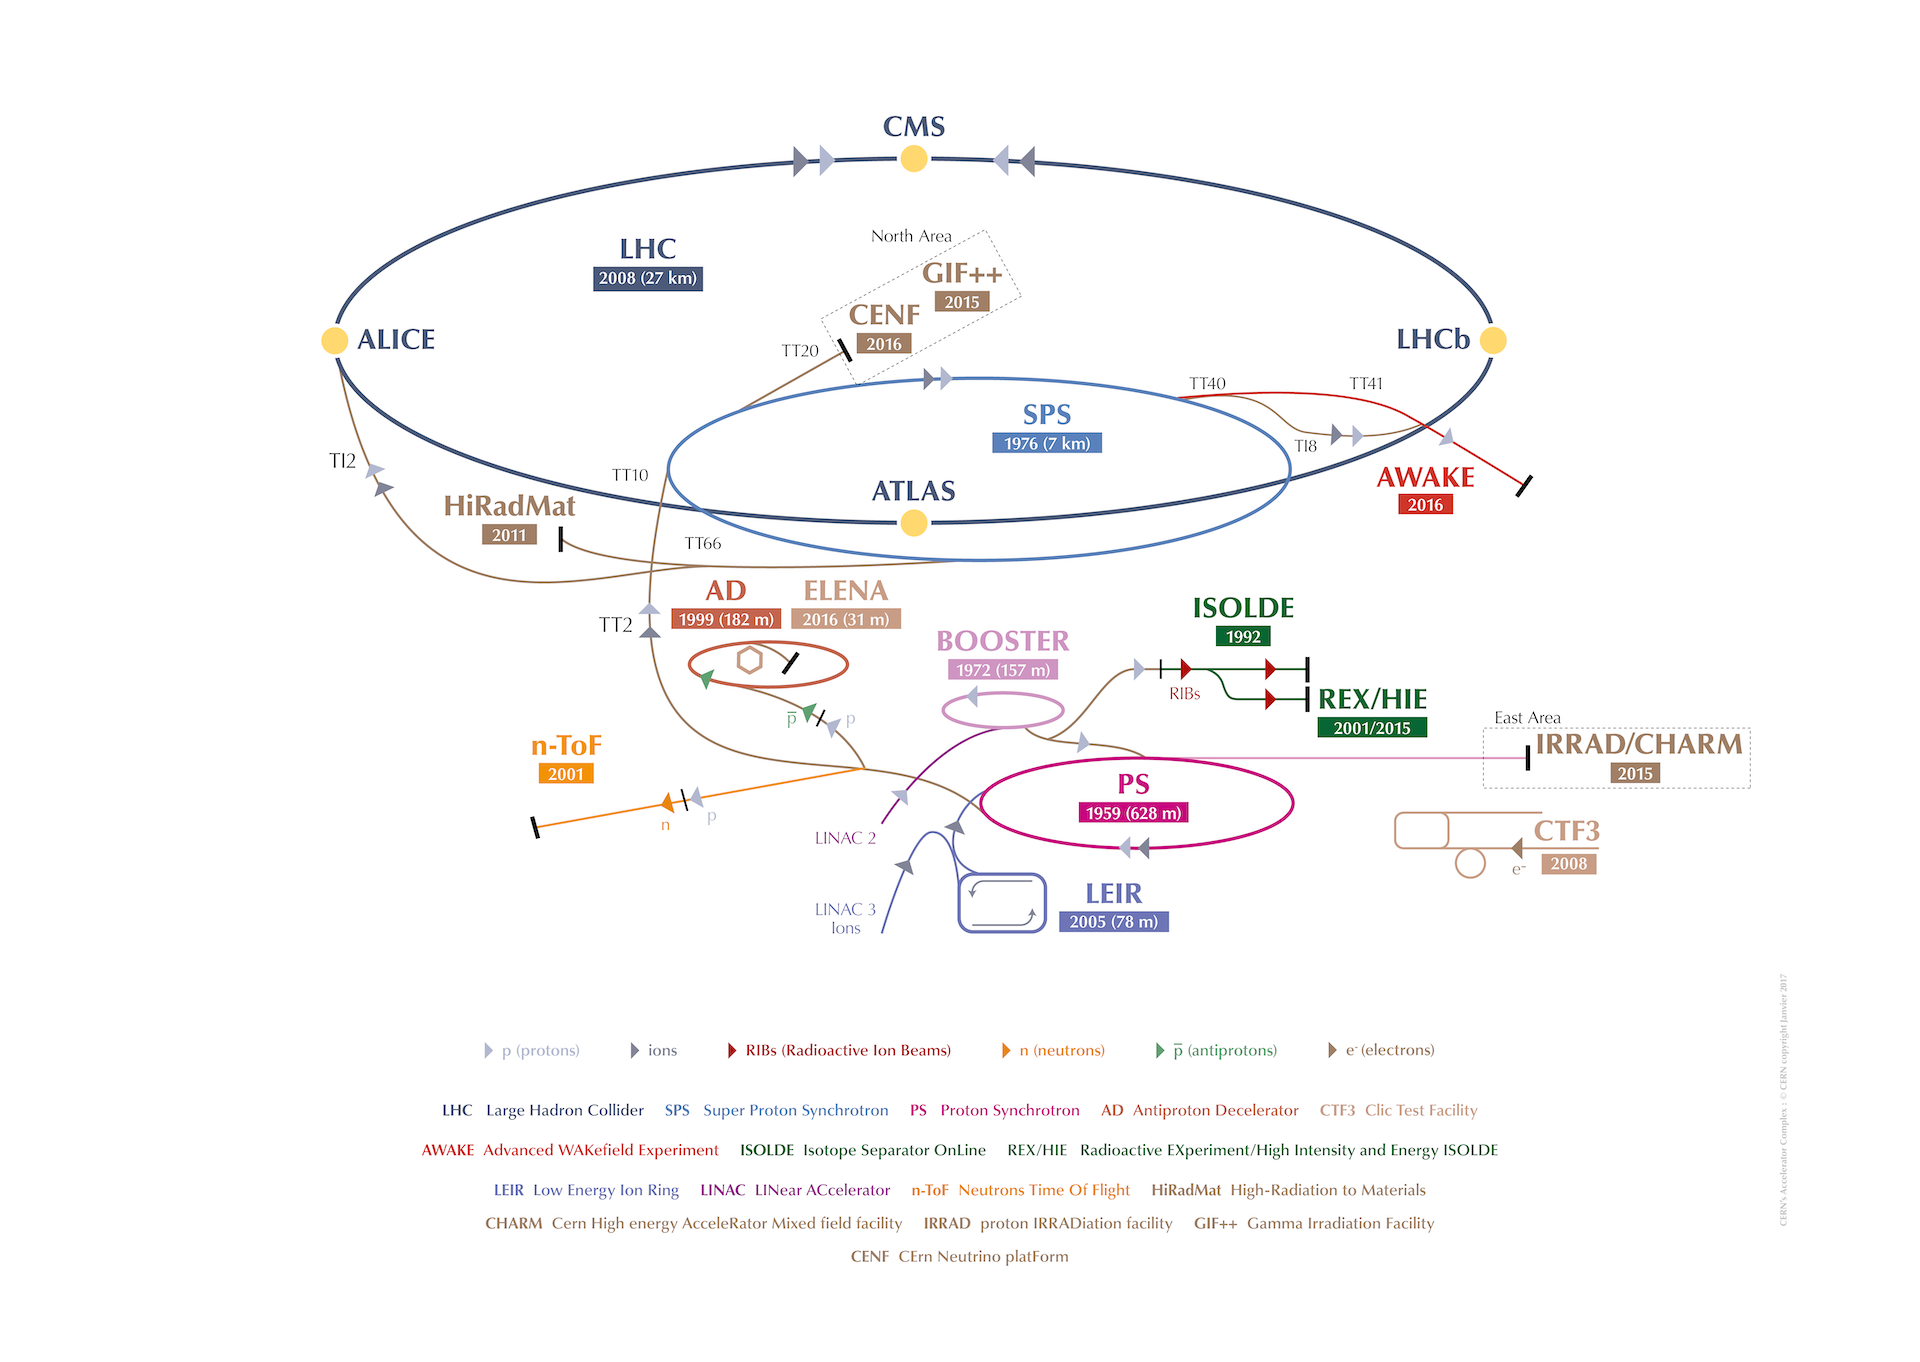
\includegraphics[width=0.9\textwidth]{pics/CernCollidersSmall}
\caption[CERN collider complex]{ A schematic view of the accelerator complex at CERN. Before particles can be injected into the LHC they require a series of preliminary? acceletarors. Until 2018 protons start their journey in LINAC2 (Linear Accelerator) and continue through the Booster, Proton Synchrotron (PS) and Super Proton Synchrotron (SPS). Between 2019 and 2020 LINAC2 will be replaced by LINAC4~\cite{CernComplex}}

\label{fig:CernComplex}
\end{figure}
\subsection{Large Hadron Collider}
\label{sec:lhc}
The Large Hadron Collider (LHC) is the largest accelerator at CERN and the largest particle collider ever built. The LHC is designed to accelerate protons up to an energy of 8\tev and lead ions up to 2.76\tev per nucleon~\cite{LHC}. The design luminosity of the LHC is $10^34 \unit{cm^{-2}s^{-1}}$. In 20xx it achieved a record peak luminosity of xxx. For lead beams the design luminosity is xxx. All this is achieved with a ring of 26.7 km, that consists of 1232 superconducting dipole magnets that keep particles in orbit. 

The particles are accelerated through the use of radio-frequency (RF) cavities. The RF are build such that the electromagnetic waves become resonant and build up inside the cavity. Charges passing through the cavity feel the overall force and are pushed forward along the accelerator. As they consist of electromagnetic waves, the field in the RF cavity oscillates. Thus particles must enter the cavity at the correct phase of oscillation to receive a forward push. When timed correctly, the particles will feel zero accelerating voltage when they have exactly the correct energy. Particles with higher energies will be decelerated  and particles with lower energies will be accelerated. This focuses particles in distinct bunches. The RF oscillation frequency at the LHC is 400.8 MHz. Thus  RF "buckets" are separated by 2.5 ns. However only 10 \% are actually filled with particles, so the bunch spacing in the LHC is 25 ns, at a bunch frequency of 40 MHz.

With 7 TeV proton beams the dipole magnets used to bend the beam must produce a magnetic field of 8.33 T. This can be only achieved through making the magnets superconducting, which requires cooling them down with helium to a temperature of 1.9 K. The 1232 dipole magnets make up roughly 2/3 of the LHC circumference. The remaining part is made up of RF cavities, various sensors and higher multipole magnets used to keep the beam focused. The most notable of these are the 392 quadrupole magnets.

The LHC is divided into octants, where each octant has a distinct function. Octants 2 and 8 are used to inject beam into the LHC from SPS. The 2 beams are crossed in octants 1,2,5 and 8. The main experiments are built around these crossing points. Octants 3 and 7 are used for beam cleansing. This is achieved through collimators that scatter particles with too high momentum or position offsets off from the beam. The RF cavities used for acceleration are located in octant 4 and octant 6 is used for dumping the beam. The beam dump is made up of two iron septum magnets, one for each beam, that will kick the beam away from machine components into an absorber when needed. 


\subsubsection{LHC experiments}
As of 2018 there are four main experiments at the LHC; ALICE, ATLAS, CMS and LHCb and three smaller ones LHCf, TOTEM and MoEDAL. ALICE will be covered in section ~\ref{sec:alice}. 

ATLAS (A Toroidal LHC ApparatuS) and CMS (Compact Muon Solenoid) are the two largest experiments at the LHC. They are both multipurpose experiments designed to be sensitive to many different possible new physics signals. The biggest discovery made by these so far is the discovery of the Standard Model Higgs boson, which was simultaneously published by the experiments in 2012 ~\cite{Atlashiggs, CMShiggs}.

The LHCb (LHC beauty) experiment ~\cite{LHCb} is made for studying the bottom (beauty) quark. Main physics goals include measurement of the parameters of CP violation with decays of hadron containing the bottom quark. One of the most important results published by LHCb is the first measurement of $B_s^0\rightarrow \mu^+ \mu^-$ decay, which was found to be in line with the Standard Model.

In addition to the four large experiments there are three smaller experiments along the LHC ring. LHCf (LHC forward) is located at interaction point 1 with ATLAS. It aims to simulate cosmic rays by the particles thrown forwards by the collisions in ATLAS.

TOTEM (TOTal Elastic and diffractive cross section Measurement) is located near the CMS experiment at point 5. This allows it to measure particles emerging from CMS with small angles. The main goals is to measure the total, elastic and inelastic cross-sections in pp collisions~\cite{TOTEM}.

The MoEDAL (Monopole and Exotics Detector At the LHC) experiment is located at the interaction point 8 together with the LHCb experiment. MoEDAL tries to measure signatures of hypothetical particles with magnetic charge, magnetic monopoles.




\subsection{ALICE}
\label{sec:alice}


\begin{figure}[htb]
\centering
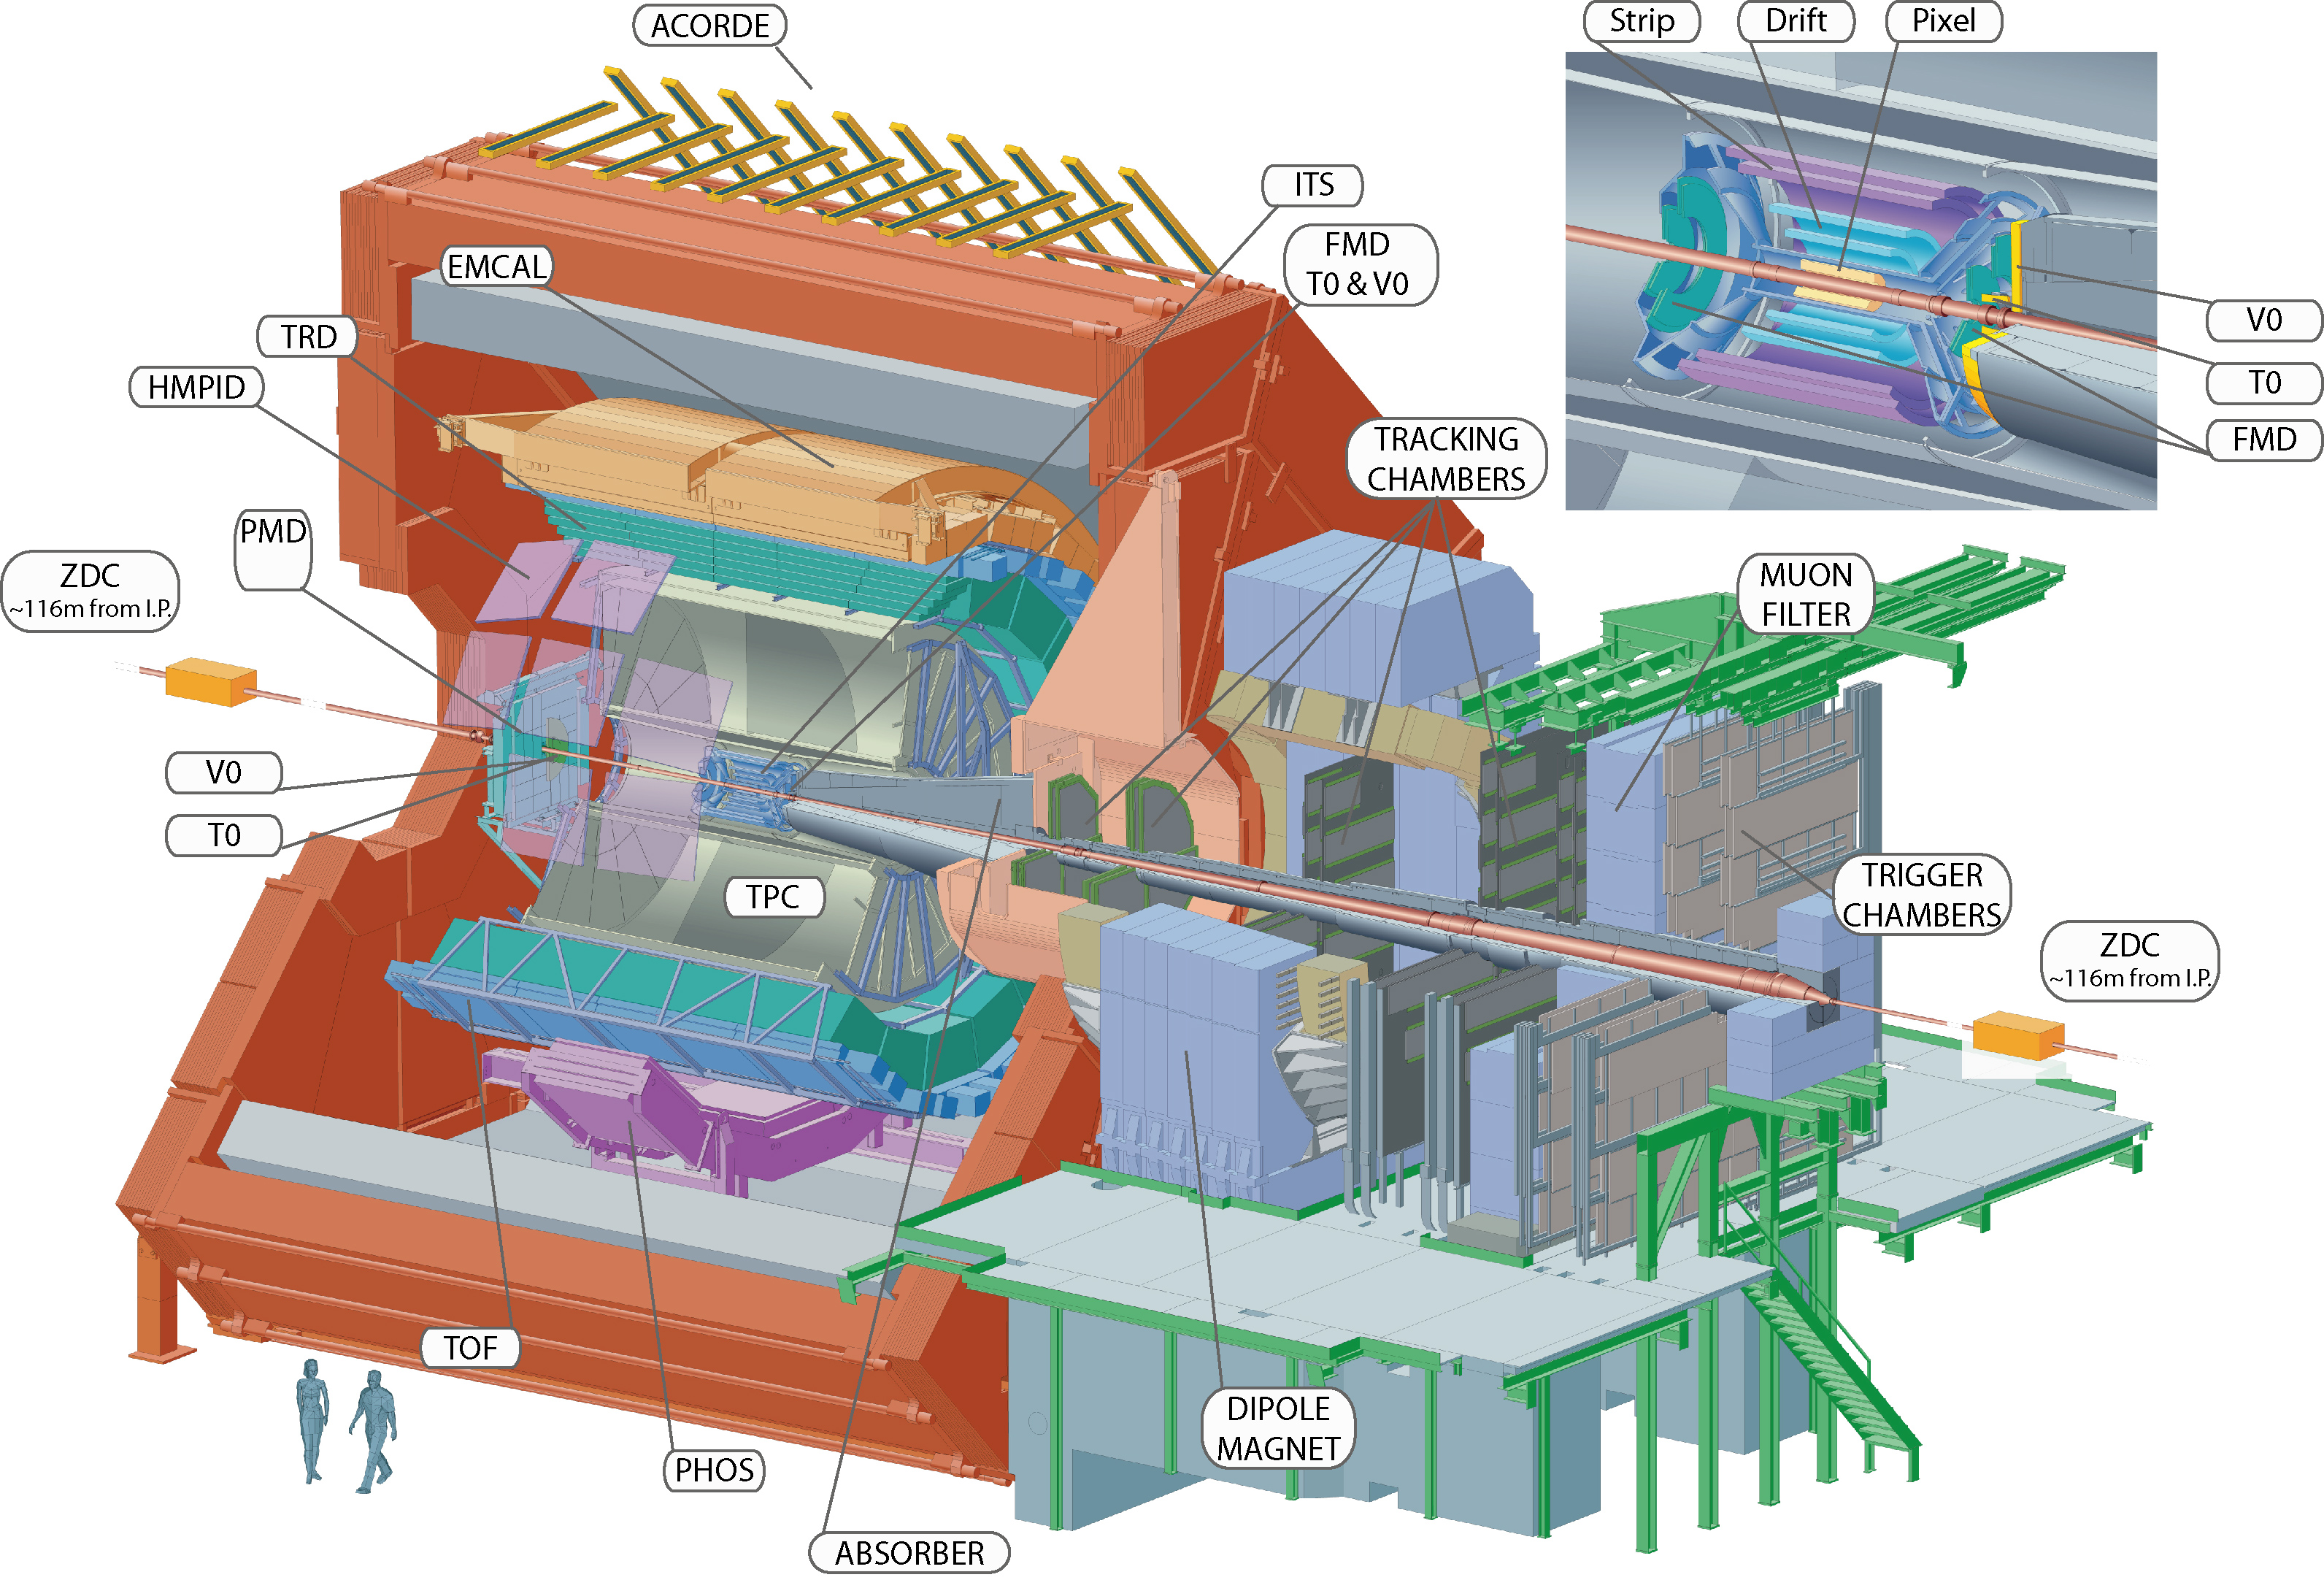
\includegraphics[width=0.95\textwidth]{pics/2012-Aug-02-ALICE_3D_v0_with_Text.jpg}
\caption[ALICE]{Schematic view of ALICE}
\label{fig:alice}
\end{figure}

ALICE (A Large Ion Collider Experiment)~\cite{ALICE} is the dedicated heavy ion experiment at the LHC. ALICE was designed to cope with the expected very high multiplicity environment of heavy ion collisions. The design allows measurement of a large number of low momentum tracks. The different detector subsystems are optimised to provide high momentum resolution and excellent particle identification capabilities over a broad range of momentum.

A schematic view of the ALICE detector in 2018 is presented in Figure ~\ref{fig:alice}. This section will go through the composition of ALICE as it has been during run 2 between 2014 and 2018. The detector will go through significant upgrades during Long Shutdown 2 in 2019-2020. As in all the major high energy physics experiments the positioning of the detectors follows a layered structure. Closest to the interaction point are the tracking detectors. The main task of these detectors is to locate the position of the primary interaction vertex accurately and to record the tracks of charged particles. To achieve this they need a very good spatial resolution close to the interaction point. Tracking detectors do not significantly alter the tracks of traversing particles. Thus they can be located in the innermost layers.

Calorimeters are designed to stop any particles hitting them and use the absorption to measure the energy of the particles. Thus they must be located behind the tracking detectors. ALICE has two separate calorimeter systems, the electromagnetic calorimeters measure mainly electrons and photons, while the muon detection system measures muons.


\subsubsection{Tracking}
\begin{figure}[htb]
\centering
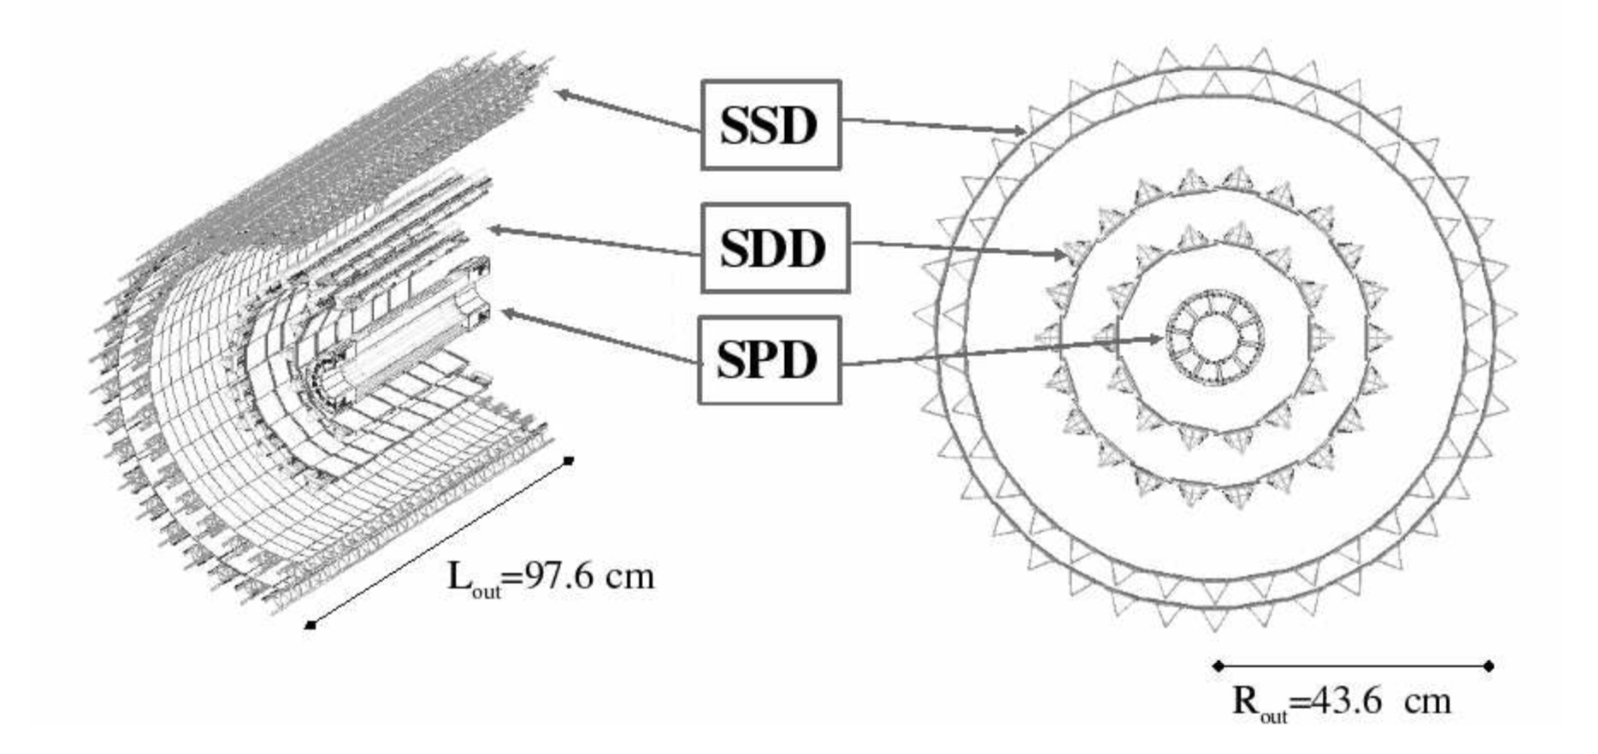
\includegraphics[width=0.95\textwidth]{pics/AliceITS}
\caption[ITS]{Schematic view of ALICE Inner Tracking System}
\label{fig:its}
\end{figure}


The main design guideline for the tracking detectors in ALICE was the requirement to have good track separation and high granularity in the high multiplicity environment of heavy ion collisions. Before LHC was built the wildest estimates put the particle density at 8000 charged particles per unit of rapidity~\cite{}. In reality the particle density turned out to be significantly smaller, about 1600 charged particles per rapidity unit.~\cite{}

The main tracking detector in ALICE is the Time Projection Chamber (TPC), discussed in more detail in section ~\ref{sec:TPC}

Between TPC and the beam pipe there is an array of six layers of silicon detectors, called the inner tracking system (ITS)~\cite{ITS}. The main tasks of the ITS are to locate the primary vertex with a resolution better than 100 $\mu m$, to reconstruct the secondary vertices from decaying particles, to track and identify particles with momenta below 200 $\mev$ and to compliment the momentum and angle measurements of TPC. During long shutdown 2 in 2019-2020 the entire ITS will be replaced~\cite{ITSupgrage}. As of 2018 the two innermost layers are made of the silicon pixel detector (SPD). As it's the closest detector to the interaction point it requires are very high spatial resolution. Thus the choice of pixel technology is natural. In heavy ion collisions the particle density is around 50 particles per $cm^2$. 

The next two layers are the silicon drift detector (SDD), which is made out of homogeneous neutron transmutation doped silicon. It is ionized when a charged particle goes through the material. The generated charge then drifts to the collection anodes, where it is measured. The maximum drift time in SDD is about 5 $\mu s$ This design gives very good multitrack capabilities and provides two out of the four $\nicefrac{dE}{dx}$ samples in the ITS.

The two remaining layers in the ITS are the silicon strip detector (SSD). The strips work in a similar way as silicon pixels, but by itself one layer only provides good resolution in one direction. Combining two crossing grids of strips provides 2 dimensional detection. Each charged particle will hit two intervening strips. The position of the hit can be deduced from the place where the strips cross each other.

\subsubsection{TPC}
\label{sec:TPC}
Time projection chamber (TPC) is a cylindrical detector filled with $ 88 m^3$ of $\mathrm{Ne-CO_2}$ (90/10 \%) gas mixture. The gas is contained in a field cage that provides an uniform electric field of $400 \nicefrac{V}{cm}$ along the z-axis (along the beam direction). Charged particles traversing through the TPC volume will ionise the gas along their path. This liberates electors that drift towards the end plates of the cylinder. 

The field cage is separated into two detection volumes by the central high voltage electrode. Both sides have a drift length of 2.5 m and inner/outer diameters of 1.2/5 m. This means the central electrode must provide a maximum potential of 100 kV to achieve the design field magnitude. The maximum time required for electrons to drift through the chamber is about 90 $\mu s$.

When electrons reach the end of the main cylinder they enter the readout chambers. The readout section of both sides consists of 18 outer chambers and 18 inner chambers. Each of them are made of multiwire proportional chambers with cathode pad readout. This design is used in many TPCs before. During Long Shutdown 2 in 2019-2020, the multiwire chambers will be replaced by Gas Electron Multipliers (GEMs, see section \ref{sec:tpcupgrade}).

The relatively slow drift time of 90 $\mu s$ is the limiting factor for the luminosity ALICE can take. The occupancy of the TPC must be kept in a manageable level. 


\subsubsection{TPC upgrade}
\label{sec:tpcupgrade}
\begin{figure}[htb]
\centering
\includegraphics[width=0.95\textwidth]{pics/alice-tpc-schematic}
\caption[TPC]{Schematic view of ALICE Time Projection Chamber}
\label{fig:tpc}
\end{figure}
During long shutdown 2 in 2019-2020 ALICE will go through significant modifications. The goal is to be able have continuous readout ~\cite{aliceupgrade} in heavy ion collisions at an interaction rate of 50 kHz. I have made a personal contribution to the quality assurance of the new GEM readout of TPC.

ALICE will add a new Forward Interaction trigger (FIT) to replace the V0 and T0 detectors. 

Additionally the current inner tracking system (ITS) will be completely replaced. The current layered structure with three different technologies will be replaced by an all pixel detector with significantly reduced pixel size. Additionally the first layer will be brought closer to the beam pipe. The new ITS will have better tracking efficiency and  better impact parameter resolution. 

The muon detection will be complimented by the Muon Forward Tracker (MFT)~\cite{mft}. Based on the same technology as the new ITS, MFT will be placed before the hadron absorber that sits in front of the existing muon spectrometer. MFT should significantly increase the signal/background ratio in heavy quark measurements.

Many subdetectors will make small improvements to enhance the readout rate. The central trigger processor will be replaced and ALICE will introduce a new framework $O^2$ that combines both online data acquisition and offline analysis.

The detector restricting the readout the most at the moment is the TPC. The current wire chamber based system  limits the readout rate to 3.5 kHz. To achieve the 50 kHz readout rate goal the wire chambers will be replaced by a Gas Electron Multiplier (GEM) based system.

TPC has a total of 36 inner and 36 outer readout chambers. Each of these will consist of 4 layers of GEM foils. The inner chambers will only have one foil for each layer. The outer chambers are separated into three sections, each with its own layer of foils. Each gem foil is made up of a 50 $\mathrm{\mu m}$ thick resistive capton layer, coated on both sides by $5 \mathrm{\mu m}$ thick layers of copper. Each foils is separated into a number (20-24) of distinct active areas. The active areas are pierced quite densely, they have 50-100 holes in the area of a single $\mathrm{mm^2}$. The density of holes changes from layer to layer. The two middle layers of foils have a larger (double) pitch (smaller hole density) while the top and bottom layers have a smaller (normal) pitch (larger hole density).

The holes have a conical shape which they acquire during a two step chemical etching process. 

The working principle of these foils is based on electrodynamics. {\color{red} elaborate}There is a large potential difference (140-400 V) applied to the two sides of the foil, which results in large field in each hole. This acts both as a lens and an amplifier for the electrons. The amplification happens inside the holes where the field is the strongest. 

As opposed to wire chambers, which typically have one voltage setting, a GEM-based detector requires several independent voltage settings: there is a drift voltage which drives the electrons from the ionisation point to the GEM, an amplification voltage, and an extraction voltage that brings electrons from the GEM exit to the readout plane. 

The GEMs are designed to minimise ion backflow to allow continuous, ungated and untriggered readout.

The purpose of the multilayered structure is to reduce the ion backflow~\cite{}; not only one layer of GEM foils will be installed, but a 4 layer stack. In the stack there are 2 standard pitch GEM foils, where the pitch size, i.e. the separation of the holes inside a foil is around 140 $\mu m$, and 2 large pitch GEM foils, there the hole spacing is two times larger, 280 $\mu m$. The two outer layers will have standard pitch and the two middle layers have large pitch. The middle layers with large pitch serve as extra insulator against the ion backflow. Additionally the setup allows operating individual GEM foils at lower voltages and still have an increase in the gain of a few orders of magnitude.

~\cite{TPCupgrade}

\subsubsection*{Quality Assurance of the GEM foils}
The GEM foils are produced at CERN, where they will undergo a basic QA (QA-B) procedure, that includes

\begin{itemize}
\item Coarse optical inspection to see any major defects, holes, cuts and discoloured regions
\item Short-term leakage current measurement
\end{itemize}

Any problems found in the basic inspection are documented for later cross-checking.


The advanced quality assurance (QA-A) is performed in two centers, one in the Helsinki Institute of Physics (HIP) and one in the Wigner Research Centre in Budapest. The QA-A procedure includes the following measurements

\begin{itemize}
\item Long-term leakage current measurement
\item High-resolution optical scanning
\item Gain uniformity check (In Budapest)
\end{itemize}

In the procedure foils are classified according to a traffic light system. Red means the foil didn't pass the basic selection criteria and thus cannot be used. Yellow means it might be usable and green means that the foil passed all evaluations.

\subsubsection{Optical scanning}
The etching process is a delicate one; many things can go wrong, that are not visible by eye in the coarse optical inspection. It is expected that the hole parameters are connected with the foil's electric properties~\cite{}, so a precise optical measurement can help in classifying the foils. For example, smaller holes create more intense and focused fields, which would result in larger amplification of their avalanche electrons, i.e. the local gain would be larger.

The foils are scanned with the help of a scanning robot. The setup along with most of the software was developed at the Detector Laboratory of the University of Helsinki~\cite{}

Each image is a false colour superposition of two images, one with foreground illumination and one with background illumination. In this way one can observe the three relevant diameters of the foil, the top, middle and bottom diameters. The background light highlights the middle holes, while the foreground illumination captures either the top or the bottom depending on the orientation of the foil as the foils are scanned from both sides. Fig.~\ref{fig:gemscan}

The setup takes images with area about $\unit[11.3]{mm} \times \unit[8.5]{mm}$, corresponding to 2560 by 1920 pixels, resulting in a total of 2000-3500 individual images for both sides of a GEM foil, depending on its type. The images are fed into neural network classifier, which identifies the holes, finds defects and extracts the hole parameters by fitting ellipses to the recognised contours. Thus every individual hole can be measured, which otherwise would be completely unfeasible as even the smallest of foils has about 10 million holes.

\begin{figure}
%\includegraphics
\caption{An example image taken of a GEM foil with false colors.}
\label{fig:gemscan}
\end{figure}

\subsubsection*{Long term HV measurement of the GEM foils}
After the optical scanning, the foils are subjected to a long term ( 5-12 hours) high voltage leakage current measurement. Each segment of the GEM foil is connected to a high voltage and the leakage current is measured separately for each segment, by the connected picoamper-meter (pA-meter)~\cite{}. The accepted leakage current in each segment is \unit[0.16]{nA}, foils with larger values are discarded. 

\subsubsection*{Gain scan}
A small subset of the foils were put through a gain scan. The gain scan could only be performed in the QA-A centre of Budapest. As the time required to scan 1 foil was several days, the gain scan couldn't be performed even for all foils in Budapest. 

The gain scan uses charged particles provided by a $\mathrm{^{55} Fe}$ source, which was placed above the foil. It emits X-ray photons with an energy of \unit[5.9]{keV}. The photons will convert to electrons in the gain scanner's $\mathrm{Ar+CO_2}$ gas mixture, either via photoelectric effect or via Compton Scattering. There electrons travel a few microns in the gas, ionising the gas along their path.

Below the GEM frame, there is a multiwire proportional pad, with perpendicular wires with a resolution of \unit[4]{mm} in $x$ and \unit[3]{mm} in $y$. Amplification is measured both with (HV) and without (reference) voltage over the GEM foil. The HV measurement is divided with the reference measurement, which results in the gain map of the GEM.

\subsubsection*{Gain correlations}

\subsubsection{Particle identification}
One guiding principle in the design of ALICE was to achieve good particle identification (PID) over  a large part of phases space and for several different particle types. In ALICE there are several detectors taking part in the identification of particles. 

One of the particle identification detectors is the transition radiation detector (TRD)~\cite{trd}. Its main task is identifying electors with momenta larger than 1 \gev. Transition radiation is produced when highly relativistic particles traverse the boundary between to media having different dielectric constants. The average energy of the emitted photon is approximately proportional to the Lorentz factor $\gamma$ of the particle, which provides an excellent way of discriminating between electrons and pion. ALICE TRD is made of a composite layer of foam and fibres. The emitted photons are then measured in six layers of Xe/CO2 filled time expansion wire chambers. 

The time of flight  (TOF) detector uses a very simple physics principle, i.e. calculating the velocity of the particle using the time of flight between two points. Combining this with the momentum of particle, obtained from the tracking detectors, one can calculate the mass of the particle, which identifies particles. The TOF detector consists of multigap resistive wire chambers. These are stacks of resistive plates spaced equally. They allow time of flight measurements in large acceptance with high efficiency and with a resolution better than 100 ps. 

The third specific particle identification detector is the high momentum particle identification (HMPID) detector. The HMPID uses a ring imaging Cherenkov counter to identify particles with momenta larger than 1 \gev. Particles moving through a material faster than the speed of light in the material will produce Cherenkov radiation. The velocity of the particle determines the angle at which the radiation is emitted. Measuring this angle gives the velocity of the particle. This can be again used to calculate the mass of the particle, if the momentum is known. In HMPID the material is a liquid radiator and the photons are measured with multiwire proportional chambers in conjunction with photocathodes. 

In addition to the specific particle identification detectors, the general purpose tracking detectors can be used for identification through the use of specific energy loss of charged particles traversing through a medium and the transition radiation emitted by charged particles when crossing the boundary between two materials. 

$\nicefrac{\mathrm{d}E}{\mathrm{d}x}$ measurements are provided by the last four layers of the ITS detector, i.e. the SDD and the SSD, thanks to their analog readout.~\cite{ALICEpid} ITS provides particle identification in the low $\pt{}$ region, up to $~ 1 \gev$, and pions reconstructed in the standalone mode can be identified down to $~100 \mev$. Similar to ITS the TPC detector provides specific energy loss measurements. TPC can identify charged hadrons up to $p_T ~ 1-2 \gev$ as well as light nuclei, He3 and He4.


\subsubsection{Electromagnetic Calorimeter}
Calorimeters are designed to measure the energy of particles. Electromagnetic calorimeters specialise in detecting particles that interact primarily through the electromagnetic interaction, namely photons and electrons. They are required in many neutral meson and direct photon analyses. In addition the energy information enhance jet measurements.

ALICE has two electromagnetic calorimeters, the photon spectrometer (PHOS)~\cite{PHOS} and the electromagnetic calorimeter (EMCal)~\cite{emcal}. PHOS is a homogeneous calorimeter that consists of scintillating $\mathrm{PbWO_4}$ crystals, which generate a bremsstrahlung  shower and produce scintillation light. The energy of the particle determines the amount of light produced. To improve the charged particle rejection, PHOS includes a charged particle veto detector (CPV)~\cite{cpv}. PHOS is built to have a very fine granularity, making it well suited for measuring direct photons and neutral mesons.

EMCal is a sampling calorimeter. It consists of layers of lead and scintillator tiles. The lead tiles produce the shower and scintillator tiles the light. The signal is then read with wavelength shifting fibres. The acceptance of EMCal in the azimuthal angle is $ 80\deg < \phi < 187 \deg$. During long shutdown 1 in 2013-2015, EMCal was extended with the di-jet calorimeter (DCal) ~\cite{DCAL}, giving an additional acceptance region of $ 260\deg < \phi < 320 \deg$. This provides partial back-to-back coverage. In comparison to PHOS, EMCal has coarser granularity, but a significantly larger acceptance, making it suitable for jet physics.

\subsubsection{Forward detectors}
ALICE includes a few small and specialised detectors of importance. The event time is determined with very good precision (< 25 ns) by the T0 detector~\cite{T0}. T0 consists of two sets of Cherenkov counters that are mounted around the beam pipe on both sides of the interaction point. T0 gives the luminosity measurement in ALICE.

Another small detector in the forward direction is the V0 detector~\cite{V0}. This consists of two arrays of segmented scintillator counters located at $-3.7 < \eta < -1.7$ and $ 2.8 < \eta < 5.1$. V0 is used as a minimum bias trigger and for rejection of beam-gas background. Particle multiplicity in the forward direction can be related to the event centrality. Thus V0 is the main detector used in centrality determination in PbPb collisions.

The multiplicity measurement of V0 is complimented by the forward multiplicity detector (FMD)~\cite{FMD}. FMD includes five rings of silicon strip detectors that make up the FMD. FMD gives acceptance in the range $-3.4 < \eta < -1.7$ and $ 1.7 < \eta < 5.0$.

During long shutdown 2 in 2019-2020, V0 and T0 will be replaced by the Fast Interaction Trigger (FIT) detector~\cite{FIT}. For historical reasons elements of FIT are also referred to as V0+ and T0+. FIT will allow centrality, event plane, luminosity and interaction time determination in the continuous readout mode, that ALICE will operate in after 2020.

For photon multiplicity measurement ALICE has the photon multiplicity detector (PMD) ~\cite{PMD}. PMD uses two planes of gas proportional counters with a cellular honeycomb structure. PMD gives the multiplicity and spatial distribution of photons in the region $2.3 < \eta < 3.7$.

On top of the ALICE magnet there is an array of 60 large scintillators called the ALICE cosmic ray detector (ACORDE) ~\cite{acorde}. ACORDE is used as a trigger for cosmic rays for calibration and alignment. 

The only hadronic calorimeters in ALICE are the zero degree calorimeters (ZDC)~\cite{zdc}, which are located next to the beam pipe in the machine tunnel about 116 m from the interaction point. There are two sets of calorimeters. One is made of tungsten, specialising in measuring neutrons, while the other, made of brass, is specialised in measuring protons. In heavy ion and especially in proton-lead collisions, ZDC gives information about the centrality of the event. ZDC is meant to detect spectators, i.e. parts of the colliding ions that do not take part in the interaction. If there are more spectators, the collisions is likely to be more peripheral.

A new detector installed during the long shutdown 1 is the ALICE diffractive detector (AD)~\cite{AD}. AD consists of two assemblies, one in each side of the interaction point, both made of two layers of scintillators. These assemblies are situated about 17 m and 19.5 m away from the interaction points. The pseudorapidity coverage is $-6.96 < \eta < -4.92 $ and $4.78 < \eta < 6.31$. AD greatly enhances ALICE's capability for diffractive physics measurements that require a large pseudorapidity gap.

\subsubsection{Muon spectrometer}
Outside the main magnet, ALICE has a spectrometer dedicated to measuring muons~\cite{MuonSpectro}. In heavy ion physics muons are mainly used to measure the production of the heavy quark resonances $\nicefrac{J}{\psi}, \Psi^{'}, \Upsilon, \Upsilon^{'}$ and $\Upsilon^{''}$.

The muon spectrometer consists of three parts, the absorber, the muon tracker and the muon trigger. The absorber is meant to remove the hadronic background as efficiently as possible. After the absorber there are ten plates of thin cathode strip tracking stations with high granularity, the muon tracker. After the muon tracker there is a layer of iron to filter out any remaining particles, other than muons. The muon trigger is located behind this layer. The trigger consists of four resistive plate chambers. 
\subsubsection{Trigger}
\subsubsection*{EMCAL trigger}


% !TEX root = thesis.tex
\section{Event and track selection}
\label{sec:selection}
The $\sqrtSnnE{5.02}$ $\pPb$ ($1.3 \cdot 10^{8}$ events, $\mathcal{L}_{\mathrm{int}} = \unit[62]{nb^{-1}}$) collisions were recorded in 2013 by the ALICE detector~\cite{aliceDetector}. The details of the performance of the ALICE detector during LHC Run~1 (2009-2013) are presented in Ref.~\cite{alicePerformance}.

%For the 2010 $\pp$ collisions, the minimum bias (MB) triggered events are required to have at least one hit from a charged particle traversing the SPD or either side of the V0. 
%The pseudorapidity coverage of the SPD is $|\eta| < 2$ in the first layer and $|\eta| < 1.5$ in the second layer. %Combining this with the acceptance of the V0, the particles are detected in the range $-3.7 < \eta < 5.1$. The minimum %bias trigger definition 



%For the $\pp$ collisions, similar track cuts as in Ref.~\cite{ALICE:2011ac} are used: at least two hits in the ITS are required, one of which needs to be in the three innermost layers, and 70 hits out of 159 are required in the TPC. In addition, the distance of the closest approach (DCA) of the track to the primary vertex is required to be smaller than $\unit{2}{cm}$ in the beam direction. In the transverse direction, a $\pt{}$ dependent cut DCA $< \unit{0.0105}{cm} + \unit{0.035}{cm} \cdot \pt{}^{-1.1}$ is used, where $\pt{}$ is measured in units of $\GeVc$. These track cuts are tuned to minimize the contamination from secondary particles.

%In $\pPb$ collisions the tracks are selected following the hybrid approach~\cite{hybridExplanation}. In this method tracks with at least one hit in the SPD and at least two hits in the whole ITS are always accepted. In addition, tracks with fewer than two hits in the ITS or no hits in the SPD are accepted, but only if an additional vertex constraint is fulfilled. In addition, the distance of the closest approach (DCA) of the track to the primary vertex is required to be smaller than $\unit{3.2}{cm}$ in the beam direction and smaller than $\unit{2.4}{cm}$ in the transverse direction. This approach is not affected by dead regions ins SPD. Thus it produces an azimuthal angle ($\varphi$) distribution that is as uniform as possible. The momentum resolutions of the two classes of particles are comparable up to $\pt{} \approx 10\;\GeVc$, but after that, tracks without ITS requirements have a worse resolution~\cite{alicePerformance,aliceBackgroundFluctuation}.




\subsection{Event selection}
This analysis uses both a minimum bias trigger and an EMCal based trigger to select the analysed events. 
%The V0 detector~\cite{forwarddetectorsTdr} provides the information for event triggering. The V0 detector consists of two scintillator hodoscopes that are located on either side of the interaction point along the beam direction. It covers the pseudorapidity region $-3.7 < \eta < -1.7$ (V0C) and $2.8 < \eta < 5.1$ (V0A).
 For the 2013 $\pPb$ collisions minimum bias events are required to have signals in both V0A and V0C. The timing difference between the two stations is also used to reduce the contamination of the data sample from beam-gas events~\cite{alicePerformance}. 

EMCal is used to provide the jet trigger used in triggered datasets. EMCal can be used to trigger on single shower deposits or energy deposits integrated over a larger area. Latter case is used for jet triggers. The EMCal trigger definition in the 2013 $\pPb$ collisions requires an energy deposit of either \unit[10]{\gev}  for the low threshold trigger or \unit[20]{\gev} for the high threshold trigger in a $32\times32$ patch size. Triggers, V0 and EMCal are discussed in more detail in sections~\ref{sec:forward},~\ref{sec:trigger} and~\ref{sec:emcal}. 

\subsection{Track reconstruction}
%\setlength{\emergencystretch}{0em}

The analysis uses charged tracks that are reconstructed with the Inner Tracking System (ITS)~\cite{aliceITS} and the Time Projection Chamber (TPC)~\cite{aliceTPC}. These are discussed in sections~\ref{sec:tracking} and~\ref{sec:TPC}. A detailed overview of track reconstruction in ALICE can be found from~\cite{alicePerformance}. 

The track reconstruction procedure is shown in Figure~\ref{fig:tracking}. The figure shows only one track, but in reality the reconstruction has to deal with many tracks. The main reconstruction of tracks starts in TPC. There are 159 tangential pad rows in the TPC readout chambers. The track reconstruction starts from the outermost layer and the hits are paired with hits in the next layer inwards, taking into account a proximity cut. When this track finding procedure hits the innermost pad row in TPC, this information is used as an initial seed for the track finding in ITS. Similar procedure of pairing adjacent layers with a proximity cut is repeated in ITS.

After the reconstruction of tracks in ITS is completed, all the tracks are extrapolated to their point of closest approach to the preliminary interaction vertex. Then the second track fitting step begins, this time starting from the interaction point and proceeding outwards. A Kalman filter~\cite{Fruhwirth:1987fm} technique is used to do the new fit using the hits found in the previous stage. This time the tracks are matched also to the other detectors in the central barrel beyond TPC. When this step is complete, a final refit from the outermost TPC pad rows towards the interaction point is performed. The final track parameters come from this refit. 

With the final track parameters the primary vertex can be determined with better accuracy than with only SPD information. The tracks are extrapolated to the nominal beam line and a weighted average of the points of closest approach determines the accurate primary vertex position.

The final step of the track reconstruction is the determination of the secondary vertices. For this, all the tracks whose distance of closest approach (DCA) to the primary vertex is larger than a defined minimum value %(?? \unit{mm} in \pPb)
are selected. For these tracks, points of closest approaches are determined for pairs of tracks. If the tracks are sufficiently close to each other and show characteristics of short lived particle decays, these points are identified as secondary vertices. 

\begin{figure}[h]
%\input{figures/tikz/tracking}
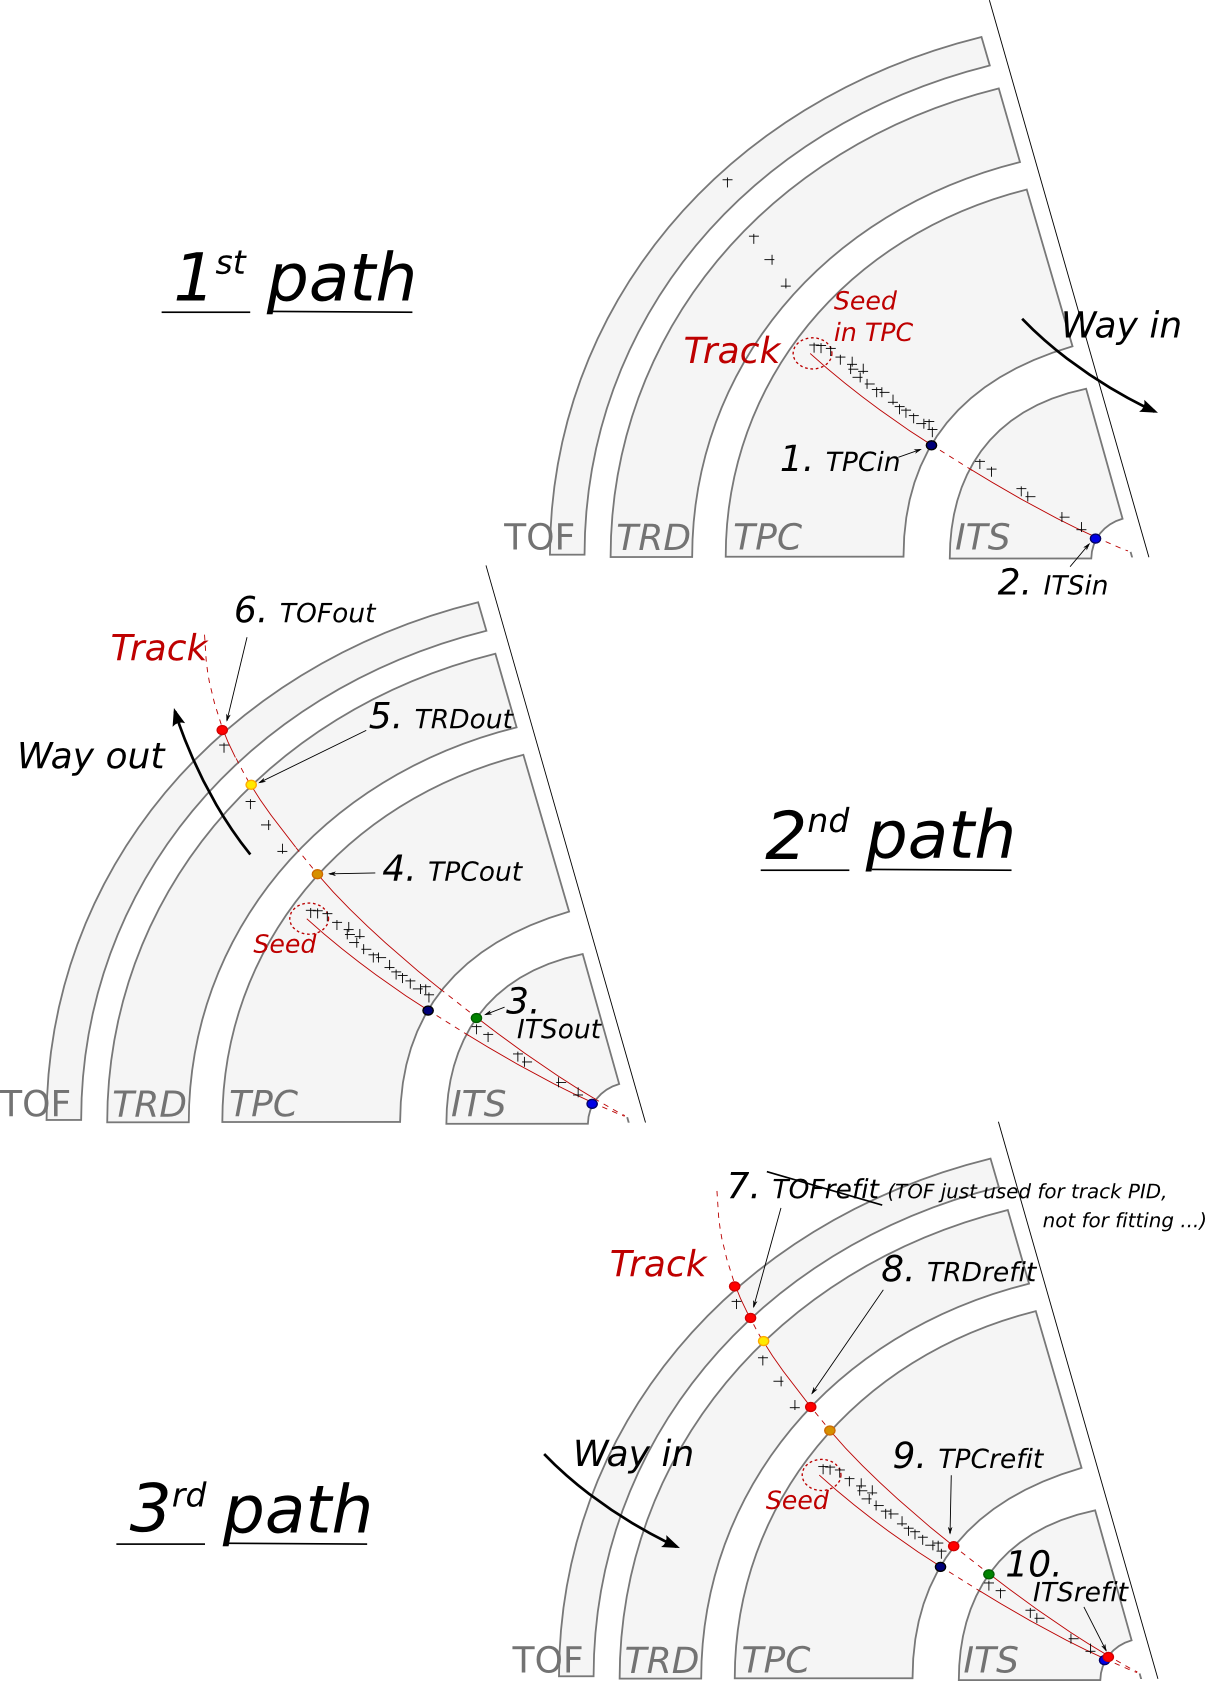
\includegraphics[width=0.9\textwidth]{pics/Schema-PcpTrackingALICE.png}
\caption{Principles of tracking in the ALICE experiment, showing the three successive paths allowing to build a track and refine its parameters. Numbers ranging from 1 to 10 mention the bits that are activated in case of success during the propagation of the Kalman filter at the considered stage. Figure from ~\cite{Maire:1984041}}
\label{fig:tracking}
\end{figure}

Combining the information from the ITS and the TPC provides a resolution ranging from $1$ to $10\,\%$ for charged particles with momenta from $0.15$ to $\unit[100]{\GeVc}$. For tracks without the ITS information, the momentum resolution is comparable to that of ITS+TPC tracks below transverse momentum $\pt{} = \unit[10]{\GeVc}$, but for higher momenta the resolution reaches $20\,\%$ at $\pt{} = \unit[50]{\GeVc}$~\cite{alicePerformance,aliceBackgroundFluctuation}. 


\subsubsection*{Track selection}
In $\pPb$ collisions the tracks are selected following the hybrid approach~\cite{hybridExplanation} which ensures a uniform distribution of tracks as a function of azimuthal angle ($\varphi$). The parameters in the approach are summarised in Table~\ref{tab:hybrid}. 

The first requirements are on the quality of the track fit in ITS and TPC. The ITS requirement only removes tracks that are clear outliers. For TPC the requirement is much more strict. For step 1 it is required that a track has 3 out of the 6 possible hits in ITS, one of which must be in the SPD. In step 2 this is replaced by an additional vertex constraint, where the primary vertex itself is added as a point to the track to improve the momentum resolution.

For the TPC, 70 crossed pad rows out of the maximum 159 is required. This measures the effective track length inside the TPC. This takes into account the possibility of having pad rows missing in the middle of the track due to charge in these clusters being below the threshold for some reason. Additionally it is required that the ratio between crossed rows and findable clusters is at least 0.8. Findable clusters are defined as the number of geometrically possible clusters which can be assigned to a track, taking into account dead zones due to chamber boundaries and limited $\eta$-acceptance. For both steps of the hybrid cut it is required that the fraction of clusters shared with several tracks is less than 40\%.

%Additionally we only accept tracks with $\left| \eta \right| < 0.8$ to avoid border effects ot the TPC acceptance $\left| \eta \right| < 0.9$ 

The remaining cuts are meant to make sure that the measured tracks are really produced in the primary collision. A track might gain a kink due to a particle scattering decay. The particle after such a kink, a kink daughter, is rejected in the cuts, as it no longer describes the properties of the primary collisions. The final cuts are on the distance of closest approach (DCA) of the track to primary vertex. To have confidence that the track comes from the primary collision, the track must be close enough to the primary vertex. The cuts are different for the distance along ($\mathrm{DCA}_{z}$) and perpendicular to ($\mathrm{DCA}_{xy}$) the beam axis.


\begin{table}
\caption{Parameters in the hybrid track cut}
\label{tab:hybrid}
\begin{tabular}{c | c | c}
Track Cut & Step 1 & Step 2 \\
\hline
$\chi^2$ / ITS cluster & < 36 & < 36 \\
$\chi^2$ / ITS cluster & < 4 & < 4 \\
Hits in ITS & 3 & 0 \\
ITS hit requirements & 1 in SPD & No requirement \\
Vertex constraint & No & Yes \\
Number of crossed rows in TPC  & 70 & 70 \\
TPC crossed rows over findable clusters & > 0.8 & > 0.8 \\
Fraction of shared TPC clusters & < 0.4 & < 0.4 \\
Kink daughters & Rejected & Rejected \\
$\mathrm{DCA}_{xy}$ & < \unit[3.2]{cm} & < \unit[3.2]{cm} \\
$\mathrm{DCA}_{z}$ & < \unit[2.4]{cm} & < \unit[2.4]{cm} \\
Other & & Rejected by step 1 \\
\end{tabular}
\end{table}



%The momentum resolutions of the two classes of particles are comparable up to $\pt{} \approx 10\;\GeVc$, but after that, tracks without ITS requirements have a worse resolution~\cite{alicePerformance,aliceBackgroundFluctuation}.



%These detectors are located inside the large solenoidal magnet, that provides a homogeneous magnetic field of \unit[0.5]{T}. Tracks within a pseudorapidity range $|\eta| < 0.9$ over the full azimuth can be reconstructed. 

%The ITS is made up of the innermost Silicon Pixel Detector (SPD), the Silicon Drift Detector (SDD) and the outermost Silicon Strip Detector (SSD). Each of these consists of two layers. The TPC is a cylinder filled with gas. Gas is ionised along the path of charged particles. Liberated electrons drift towards the end plates of the cylinder where they are detected. 


\FloatBarrier
\subsection{Cluster selection}
Neutral particles used in jet reconstruction are reconstructed by the Electromagnetic Calorimeter (EMCal)~\cite{Cortese:2008zza}. The EMCal covers an area with a range of $|\eta| < 0.7$  in pseudorapidity and $ 100 \deg $ in azimuth. EMCal is complimented with the Dijet Calorimeter (DCal)~\cite{DCAL} and Photon Spectrometer (PHOS)~\cite{PHOS} that are situated opposite of the EMCal in azimuth. PHOS covers 70 degrees in azimuth and $\left| \eta \right| < 0.12$. The DCal is technologically identical to EMCal. The DCal coverage spans over 67 degrees in azimuth, but in pseudorapidity the mid region is occupied by the PHOS. In between PHOS and DCal active volumes, there is a gap of 10 cm. DCal is fully back-to-back with EMCal.

\begin{table}[tb] 
\centering
\caption{Parameters used in the EMCal clusteriser}
\label{tab:clusters}
\begin{tabular}{| c | c |}
Setting & Value \\
Clusteriser seed & 0.2 \unit{\mev} \\
Clusteriser cutoff & 0.05 \unit{\mev} \\
Cells in cluster & > 1 \\
Track matching radius & 0.025 \\
Fiducial cut & 1 tower \\
Exotic cut & 0.97 \\
Minimal cluster Energy & 0.3 \unit{\gev}
%Maximum pair asymmetry & 0.8 \\
\end{tabular}
\end{table}

The clusters used in the analysis were obtained from the EMCal clusteriser. The parameters used in the clusteriser are summarised in Table~\ref{tab:clusters}. The clusteriser  searches for a tower with energy deposit greater than a defined seed energy and merges all surrounding (sharing a side) towers with energy deposit higher than a defined threshold. In the next step all towers sharing a side with already included towers are added, again requiring that the energy deposits exceeds the threshold. The algorithm can identify local minima and halts the clustering in case that the neighbouring tower energy is higher. Already clustered towers are removed from the pool, so one tower can only be clustered once. 

Highly energetic calorimeter hits should spread into several towers as the electromagnetic shower evolves. However, some clusters with high energy have their energy located in a single tower. These are believed to come from a slow neutron hitting the APD readout of the towers. They are referred to as exotic clusters. The measure of exoticity is denoted as 
\begin{equation}
1 -\frac{E_\mathrm{cross}}{E_\mathrm{max}},
\end{equation}

\noindent where $E_\mathrm{max}$ is the energy in the most energetic tower and $E_\mathrm{cross}$ is the sum of the four towers neighbouring the most energetic one. The closer this is to 1, the more exotic the cluster is and the larger the probability that it is fake. Cut of 0.97 has been adopted as default for analyses using EMCal, including the one presented in this thesis. Any clusters above this cut are removed.

A method of matching the cluster position to TPC track extrapolation is used to suppress charged hadron contribution to hits in EMCal. Tracks identified by the tracking detectors are extrapolated close to the EMCal surface, where the closest cluster is found and the track extrapolation is continued until reaching the same depth as the cluster. The remaining distance in between the extrapolated track and the cluster is then used to reject hadronic hits. Clusters matched to charged tracks are removed from the analysis as well as clusters being identified as fake. 








%The combination of charged tracks with  $\pt{} > \unit[0.15]{\GeVc}$ and neutral particles with $\pt{} > \unit[0.30]{\GeVc}$ is used to construct jets. 


%\subsection{statistics}
%Number of jets in different datasets and with different jet finders is shown in Table~\ref{tab:stats}. Background statistics for number of background cones (number of jets minus number of discarded cones) are shown in Table~\ref{tab:bgstats}. Ratio of background cones to number of jets is shown in Table~\ref{tab:bgratio}. The likelihood of having to discard a jet from background calculation is about 1-2\%.
%\begin{table}[h]
%\caption{Number of found jets by dataset and jet $\pt{}$ bin}
%\tiny
%\begin{tabular}{c | c | c | c | c | c | c | c | c | c}
%Jet $\pt{}$   &     5-10 & 10-20  & 20-30 & 30-40 & 40-60 & 60-80 & 80-100 & 100-150 & 150-500 \\
%MBFullR04 & 4969393 & 621753 & 32552 & 5584 & 1974 & 310 & 90 & 37 & 5 \\
%MBFullR05 & 4750567 & 826598 & 42373 & 5543 & 1719 & 276 & 73 & 29 & 3 \\
%MBChargedR04 & 3144538 & 673419 & 37783 & 4121 & 1009 & 148 & 36 & 12 & 1 \\
%MBChargedR05 & 2229247 & 175763 & 7961 & 1270 & 410 & 61 & 12 & 3 \\
%TriggeredFullR04 & 187557 & 115927 & 78138 & 51317 & 39262 & 8621 & 2409 & 1167 & 171 \\
%TriggeredFullR05 & 99991 & 77147 & 48612 & 34325 & 28104 & 6342 & 1726 & 794 & 104 \\
%TriggeredChargedR04 & 37411 & 29945 & 18186 & 13148 & 11142 & 2517 & 675 & 326 & 44 \\
%TriggeredChargedR05 & 433155 & 175031 & 54789 & 19776 & 10626 & 1983 & 457 & 194 & 15 \\
%\end{tabular}
%\label{tab:stats}
%\end{table}
%
%\begin{table}[h]
%\caption{Number of background cones used in perpendicular cone background calculation}
%\label{tab:bgstats}
%\tiny
%\begin{tabular}{c | c | c | c | c | c | c | c | c | c}
%Jet $\pt{}$     &   5-10 & 10-20  & 20-30 & 30-40 & 40-60 & 60-80 & 80-100 & 100-150 & 150-500 \\
%MBFullR04 & 4947583 & 617895 & 32357 & 5548 & 1965 & 310 & 90 & 37 & 5 \\
%MBFullR05 & 4710217 & 815461 & 41584 & 5439 & 1698 & 273 & 73 & 29 & 3 \\
%MBChargedR04 & 3117495 & 661106 & 36739 & 4014 & 988 & 144 & 36 & 12 & 1 \\
%MBChargedR05 & 2195286 & 172919 & 7860 & 1249 & 406 & 61 & 12 & 3 \\
%TriggeredFullR04 & 186574 & 115376 & 77949 & 51216 & 39196 & 8603 & 2405 & 1167 & 171 \\
%TriggeredFullR05 & 99102 & 76462 & 48320 & 34216 & 28038 & 6334 & 1722 & 794 & 103 \\
%TriggeredChargedR04 & 37160 & 29543 & 17988 & 13099 & 11129 & 2515 & 675 & 326 & 44 \\
%TriggeredChargedR05 & 313421 & 140707 & 45229 & 16243 & 8709 & 1604 & 377 & 154 & 14 \\
%\end{tabular}
%\end{table}
%
%\begin{table}[h]
%\caption{Ratio of background cone number to number of jets}
%\label{tab:bgratio}
%\tiny
%\begin{tabular}{c | c | c | c | c | c | c | c | c | c}
%MBFullR04 & 99.56\% & 99.38\% & 99.40\% & 99.36\% & 99.54\% & 100.00\% & 100.00\% & 100.00\% & 100.00\% \\
%MBFullR05 & 99.15\% & 98.65\% & 98.14\% & 98.12\% & 98.78\% & 98.91\% & 100.00\% & 100.00\% & 100.00\% \\
%MBChargedR04 & 99.14\% & 98.17\% & 97.24\% & 97.40\% & 97.92\% & 97.30\% & 100.00\% & 100.00\% & 100.00\% \\
%MBChargedR05 & 98.48\% & 98.38\% & 98.73\% & 98.35\% & 99.02\% & 100.00\% & 100.00\% & 100.00\% \\
%TriggeredFullR04 & 99.48\% & 99.52\% & 99.76\% & 99.80\% & 99.83\% & 99.79\% & 99.83\% & 100.00\% & 100.00\% \\
%TriggeredFullR05 & 99.11\% & 99.11\% & 99.40\% & 99.68\% & 99.77\% & 99.87\% & 99.77\% & 100.00\% & 99.04\% \\
%TriggeredChargedR04 & 99.33\% & 98.66\% & 98.91\% & 99.63\% & 99.88\% & 99.92\% & 100.00\% & 100.00\% & 100.00\% \\
%TriggeredChargedR05 & 72.36\% & 80.39\% & 82.55\% & 82.13\% & 81.96\% & 80.89\% & 82.49\% & 79.38\% & 93.33\% \\
%\end{tabular}
%\end{table}
%
%


\clearpage
\section{Analysis method}
\label{sec:methods}
\subsection{Jet Finding}
The analysis uses reconstructed jets as estimates of the original parton. Jet reconstruction essentially combines nearby tracks into jets. 

Collisions between hadrons are never as clean as electron-electron collisions. Even for a proton-proton collision there are participant partons, that will produce a soft background in addition to the hard scattering products. Jet reconstruction must deal with this soft background. The reconstruction is never perfect, one can have uncorrelated tracks that get included in the jet and some tracks originating from the parton are missed by the reconstruction. There are several methods to perform the reconstruction, all of which require some kind of size parameter, which cuts out jet participants too far from the jet axis. The tracks that are grouped into a jet are referred to as jet constituents. 

In each collision event, the jets are reconstructed using FastJet~\cite{fastjet} with the anti-$\kt{}$ algorithm~\cite{antikt}. Jets for R=0.4 are selected in $\left| \eta \right| < 0.25 $ to satisfy the fiducial acceptance of the EMCal. In jet reconstruction both charged tracks with $\pt{}>0.15\,\GeVc$ and neutral clusters with $\pt{}>0.30\,\GeVc$ are considered. Clusters that match charged tracks are removed before jet reconstruction. The analysis is then performed by analysing the charged jet constituents and results are presented in terms of the jet transverse momentum $\pt{,jet}$. 

\subsubsection{Anti \texorpdfstring{\kt{}}{kT} algorithm}
Jets are reconstructed using the anti-$\kt{}$ algorithm~\cite{antikt}. The algorithm works by trying to undo the splittings through combining protojets. First the algorithm creates a list of protojets. At the beginning the list is populated by converting each track in the event into a protojet. Then the algorithm proceeds by combining these protojets. A simplified picture of the process for a limited number of tracks is shown in Figure~\ref{fig:ktalg}

The algorithm calculates distance measures for each individual protojet and for each possible pair of protojets. For individual protojets this depends on the transverse momentum of the track.

\begin{equation}
\kt{,i}^2=\pt{,i}^{2p}
\end{equation}

\noindent For each pair of protojets the distance measure is calculated as

\begin{equation}
\kt{i,j}^{2}=\min\left(\pt{i}^{2p},\pt{j}^{2p}\right)\frac{\Delta R^2_{i,j}}{D^2},
\end{equation}
\nopagebreak
\noindent where
 \nopagebreak
 \begin{equation}
 R_{i,j}=\left(\phi_i-\phi_j\right)^2+\left(y_i-y_j\right)^2.
 \end{equation}

If $\kt{i}$ is the smallest quantity then the protojet is a jet and it is removed from further consideration. If \kt{i,j} is the smallest quantity the two protojets $i$ and $j$ are merged. This is repeated until no protojets are left.

The choice of the power $p$ in the distance measure depends on the algorithm used
\begin{itemize}
\item $p=1$:~$\kt{}$ algorithm
\item $p=0$:~Cambridge Aachen algorithm
\item $p=-1$:~anti-$\kt{}$ algorithm
\end{itemize}

With the choice $p=-1$ in anti-$\kt{}$ algorithm, the softest splittings are undone first. One consequence of the power choice in the anti-$\kt{}$ algorithm is that reconstructed jets have a shape close to circular.


   \begin{figure}
\centering
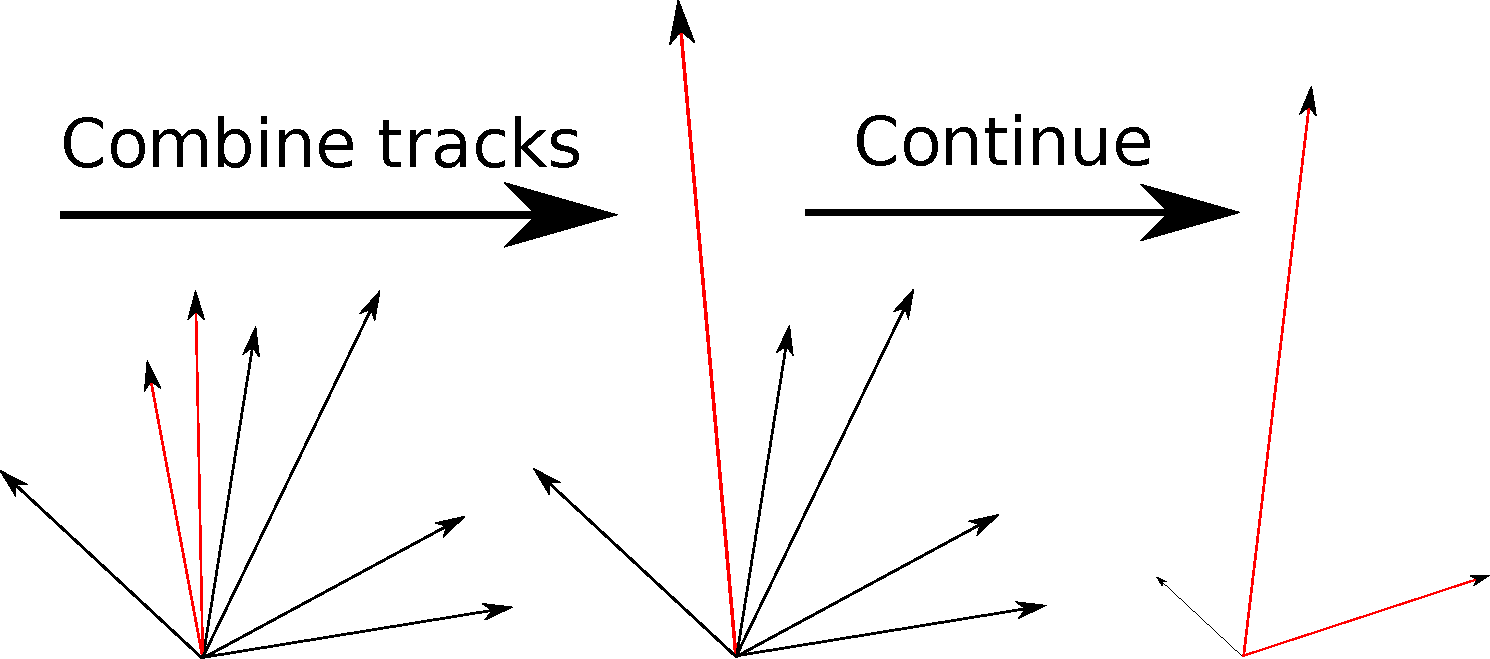
\includegraphics[width=0.8\textwidth]{pics/ktalg.pdf}
    \caption{A simple example of the antil-$\kt{}$ algorithm in progress. The red tracks in the leftmost figure are identified to have the smallest $k_{T,i}$ in the event and are combined into the red track of the middle figure. As this continues the remaining tracks are added to this or other jets. One tracks was deemed to be isolated enough to be counted as a protojet by itself. Note that the rightmost figure is zoomed out.}
    \label{fig:ktalg}
  \end{figure}






\subsection{Definition of \texorpdfstring{$\jt{}$}{jT} }
The reconstructed jet axis is used for $\jt{}$ reference. Any charged track within a fixed cone with radius $R$ is taken as a jet constituent, as opposed to using the constituent list provided by the jet algorithm. Anti-$\kt{}$ produces jets that are very circular in shape. Thus this doesn't change the constituent list considerably. Calorimeter clusters are used only in jet reconstruction.

The jet fragmentation transverse momentum, $\vec{\jt{}}$, is defined as the component of the constituent track momentum, $\vec{p}_{\mathrm{track}}$, transverse to the jet momentum, $\vec{p}_{\mathrm{jet}}$. It represents the transverse kick with respect to the initial hard parton momentum that is given to a fragmenting particle during the fragmentation process, which is a measure of the momentum spread of the jet fragments.

   \begin{figure}
    \begin{center}
      \includegraphics[width = 0.60\textwidth]{figures/tikz/jtdef}
    \end{center}
    \caption{Illustration of $\vjt{}$. The jet fragmentation transverse momentum, $\vjt{}$, is defined as the transverse momentum component of the track momentum, $\vec{p}_{\mathrm{track}}$, with respect to the jet momentum, $\vec{p}_{\mathrm{jet}}$.}
    \label{fig:jtdefinition}
  \end{figure}

The resulting $\vjt{}$ is illustrated in~\fig{fig:jtdefinition}. The length of the $\vjt{}$ vector is

  \begin{equation}
    \jt{} = \frac{|\vec{p}_{\mathrm{jet}} \times \vec{p}_{\mathrm{track}}|}{|\vec{p}_{\mathrm{jet}}|} \,.
  \label{eq:jtdefinition}
  \end{equation}


 
 
Resulting $\jt{}$ distributions are shown as 
\begin{equation}
\frac{1}{\jt{}}\frac{\mathrm{d}N}{\mathrm{d}\jt{}}
\end{equation}
distributions. The logic behind this is that $\jt{}$ is inherently a two-dimensional observable, comprised of $\jt{x}$ and $\jt{y}$ components. So the actual physical observable would be 
 
 \begin{equation}
 \frac{\mathrm{d}^2N}{\mathrm{d} \jt{x} \mathrm{d} \jt{y}}
 \end{equation}

\noindent Changing into polar coordinates with $\jt{r} = \jt{}$ and $\theta$ gives
 \begin{equation}
 \frac{\mathrm{d}^2N}{\jt{} \mathrm{d} \jt{} \mathrm{d} \theta},
 \end{equation}

\noindent where $\jt{}$ over the azimuth $\theta$ should stay constant and it can be integrated over, which gives 
\begin{equation}
\frac{1}{2\pi}\frac{\mathrm{d}N}{\jt{} \mathrm{d} \jt{}}.
 \end{equation}
 
Results of the raw inclusive $\jt{}$ distribution in four $\pt{,jet}$ bins with background are shown in Figure~\ref{fig:inclusive}. Background, i.e. the contribution from the underlying event, is further discussed in Section~\ref{sec:bg}
 
 \begin{figure}
\centering
\begin{subfigure}{0.95\textwidth}
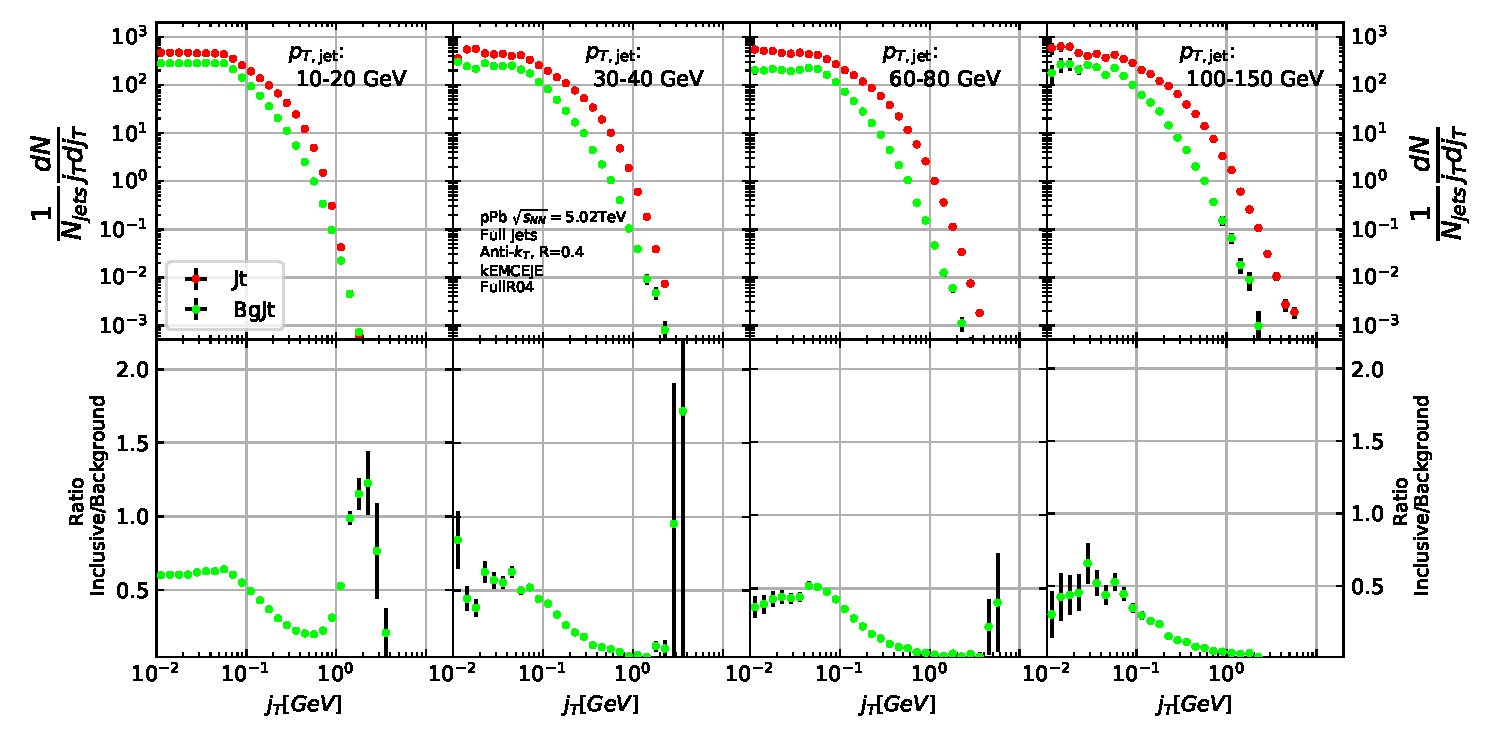
\includegraphics[width=\textwidth]{results/MixedFullJetsR04JetConeJtInclusive.pdf}
%Tag 20170810 python2.7 Python/InclusiveWithBackground.py legotrain_CF_pPb-1053_20170223-2002_LHC13bcde.root
\end{subfigure}
\caption{Inclusive $\jt{}$ with background}
\label{fig:inclusive}
\end{figure}

 
\subsection{Unfolding detector effects}
The raw inclusive $\jt{}$ distributions are corrected for the detector inefficiency with an unfolding procedure. The procedure uses response matrices obtained from a \textsc{Pythia}~\cite{introPythia81} simulation.

Measured distributions are affected by two main factors; Limited acceptance - The probability to observe a given event is less than one and limited resolution - Quantity $x$ cannot be determined exactly, but there is a measurement error. True $f(x)$ and measured $g(y)$ distributions are connected by a convolution integral. Including statistical fluctuations this becomes
\begin{equation}
\hat g(y) = \int_a^b A\left(y,x\right) f(x) dx + \epsilon(y),
\end{equation}

\noindent where A is the detector response obtained by (for example) Monte Carlo simulations and $\epsilon(y)$ is the term coming from statistical fluctuations.
If $x$ and $y$~ are discrete variables we have
\begin{equation}
\hat g_i = \sum_{j=1}^m A_{ij}f_j+\epsilon_i,
\end{equation}

where $i$ and $j$ give the $\jt{}$ bins in the true and measured distributions. $f_j$ and $g_i$ give the counts in these bins.
\noindent Or in matrix form
\begin{equation}
\hat g = Af+\epsilon,
\end{equation}
\noindent where $\hat g$ and $f$ are vectors corresponding to the measured and true histograms. If the only detector effect is limited acceptance, $A$ is a diagonal matrix, i.e. $A_{ij}=0$ for $i\neq j$. We want to deduce the true distribution $f$, when the measured distribution $g$ is known. In a general discrete case the (naive) solution is obtained by the inverse matrix
\begin{equation}
\hat f = A^{-1}\hat g 
\end{equation}
However this usually leads to oscillating solutions and determining the inverse matrix can be difficult.

Two common methods to perform this inversion are Bayesian and SVD unfolding methods. Often the solution requires some additional {\emph{ a priori}} information. For example the solution should be smooth in most cases.

\subsubsection{Bayesian unfolding}
The bayesian (iterative) method is based on the Bayes formula~\cite{ADictionaryofStatistics}.
\begin{equation}
P\left(C_i |E_j\right)=\frac{P\left(E_j |C_i\right)P_0\left(C_i\right)}{\sum_{l=1}^{n_C}P\left(E_j |C_l\right)P_0\left(C_l\right)},
\end{equation}

\noindent i.e. the probability of Cause $C_i$ ("truth") given Effect $E_j$ ("observed") is proportional to the probability of observing $E_j$ given $C_i$, $P\left(E_j |C_i\right)$ (response matrix) and the true distribution $P_0\left(C_i\right)$.

In the unfolding procedure $P_0$ is given some starting distribution, either a uniform distribution or some guess of the final distribution. Taking into account the inefficiency this gives 

\begin{equation}
\hat n\left(C_i\right) = \frac{1}{\epsilon_i} \sum_{j=1}^{n_E}n\left(E_j\right)P\left(C_i | E_j\right),
\end{equation}
%\item First calculate $P\left(C_i |E_j\right)$ with the uniform distribution
\noindent where 
\begin{equation}
P\left(C_i |E_j\right)=\frac{P\left(E_j |C_i\right)P_0\left(C_i\right)}{\sum_{l=1}^{n_C}P\left(E_j |C_l\right)P_0\left(C_l\right)},
\end{equation}


\noindent and $n\left(E_j\right)$ are the observed frequencies. First  $P\left(C_i |E_j\right)$ is calculated with the uniform distribution or best guess of the shape of the distribution. This is then used to calculate the new distribution $\hat P\left(C_i\right)$
\begin{equation}
\hat N_{true} = \sum_{i=1}^{n_C} \hat n\left(C_i\right),\,\hat P\left(C_i\right) = P\left(C_i | n\left(E\right)\right) = \frac{\hat n\left(C_i\right)}{\hat N_{true}}
\label{eq:unfolded}
\end{equation}

$P_0$ is then replaced with $\hat P$ and the procedure is repeated until an acceptable solution is found. One way to gauge the acceptability is measuring the change between iterations. Initially there is a large change between iterations, but it should get small when close to the final distribution. The number of iterations should be as low as possible, as the errors increase when going further in the iterations, but the number of iterations must be high enough so that the correct distribution is extracted. 

The bayesian procedure alongside with the SVD unfolding method are implemented in the RooUnfold package~\cite{roounfold}, which is used to perform the unfolding in practice. SVD unfolding is another procedure that utilises the Singular Value Decomposition (SVD) of the response matrix to find the inverse of the response matrix~\cite{Hocker:1995kb}.
 
 \subsubsection*{Error propagation in the Bayesian procedure }
 The measured distribution has some statistical uncertainty, this should be reflected in the unfolded distribution. Additionally the response matrix may have some uncertainty if the statistics used in the Monte Carlo simulation were limited. 
 
For errors originating from the measured distribution RooUnfold uses the error propagation matrix 

\begin{equation}
\frac{\partial \hat n\left(C_i\right)}{\partial n\left(E_j\right)} = M_{ij} + \frac{\hat n\left(C_i\right)}{n_0\left(C_i\right)}\frac{\partial n_0\left(C_i\right) }{\partial n\left(E_j\right) } - \sum_{k=1}^{n_E}\sum_{l=1}^{n_C} \frac{n\left(E_k\right) \epsilon_l}{n_0\left(C_l\right)} M_{ik} M_{lk} \frac{\partial n_0 \left(C_l\right)}{\partial n\left(E_j\right)},
\end{equation} 
 
\noindent where $\hat n \left(C_i\right)$ is the unfolded result from Eq.~\ref{eq:unfolded}. This depends upon the matrix $\frac{\partial n_0\left(C_i\right)}{\partial n\left(E_j\right) }$, which is $\frac{\partial \hat n\left(C_i\right) }{\partial n\left(E_j\right) }$ from the previous iteration. In the first iteration, $\frac{\partial n_0\left(C_i\right) }{\partial n\left(E_j\right) }=0$ and $\frac{\partial \hat n\left(C_i\right) }{\partial n\left(E_j\right) } = M_{ij}$.
 
 The error propagation matrix $V$ is used to obtain the covariance matrix on the unfolded distribution 
 
 \begin{equation}
 V\left(\hat n\left(C_k\right), \hat n\left(C_l\right)\right) = \sum_{i,j=1}^{n_E} \frac{\partial \hat n\left(C_k\right) }{\partial n\left(E_i\right) }  V\left(\hat n\left(E_i\right), \hat n\left(E_j\right)\right)  \frac{\partial \hat n\left(C_l\right) }{\partial n\left(E_j\right) },
 \end{equation}
 
\noindent where $V\left(\hat n\left(E_i\right), \hat n\left(E_j\right)\right)$ is the covariance matrix of the measurements. In counting experiments common in particle physics, each bin is independently Poisson distributed, with
 
 \begin{equation}
 V\left(\hat n\left(E_i\right), \hat n\left(E_j\right)\right) = n\left(E_i\right) \delta_{ij}
 \end{equation}
 
 \noindent The error propagation matrix for the response matrix is 
 
 \begin{multline}
 \frac{\partial \hat n\left(C_i\right)}{\partial P \left(E_j| C_k\right)} = \frac{1}{\epsilon_i}\left(\frac{n_0 \left(C_i\right) n\left(E_j\right)}{f_j} - \hat n \left(C_i\right) \right) \delta_{ik} - \frac{n_0 \left(C_k\right) n\left(E_j\right)}{f_j} M_{ij} + \\
  \frac{\hat n\left(C_i\right)}{n_0\left(C_i\right)} \frac{\partial n_0\left(C_i\right)}{\partial P \left(E_j| C_k\right)} - \frac{\epsilon_i}{n_0\left(C_i\right)} \sum_{l=1}^{n_E}\sum_{r=1}^{n_C} n\left(E_l\right) M_{il} M_{rl} \frac{\partial n_0 \left(C_r \right)}{\partial P \left(E_j| C_k\right)},
 \label{eq:responseerror}
 \end{multline}
 
\noindent where $ \frac{\partial n_0\left(C_i\right)}{\partial P \left(E_j| C_k\right)}$ is the error propagation matrix from the previous iteration, $\frac{\hat n\left(C_i\right)}{\partial P \left(E_j| C_k\right)}$. For the first iteration, this is zero and the final two terms in Eq.~\ref{eq:responseerror} disappear.
 
 The covariance matrix due to these errors is given by
 
 \begin{equation}
 V\left(\hat n\left(C_k\right), \hat n\left(C_l\right)\right) = \sum_{j,s=1}^{n_E} \sum_{i,r=1}^{n_C} \frac{\partial \hat n\left(C_k\right) }{\partial P\left(E_j | C_i\right) }  V\left(P\left(E_j | C_i\right), P\left(E_s | C_r\right) \right)  \frac{\partial \hat n\left(C_l\right) }{\partial P\left(E_s | C_r\right) },
 \end{equation}
 
\noindent where $V\left(P\left(E_j | C_i\right), P\left(E_s | C_r\right) \right)$ can be taken as multinomial, Poisson or other distribution.
 
\subsubsection{Toy Monte Carlo} 
 A toy Monte Carlo simulation was performed to see the performance of unfolding in an ideal case.
The simulations samples jet $\pt{}$ values from the observed $\pt{}$ distribution. Starting from this $\pt{}$ the simulations starts creating tracks with 
\begin{equation}
p_{\mathrm{track}} = z_\mathrm{track} \pt{,jet}
\end{equation}

\noindent where $z_\mathrm{track} $ is sampled from the observed $z$ distribution. Tracks are given random $\eta$ and $\phi$ values from uniform distributions centred at 0. All tracks below \unit[0.15]{\gev} are discarded. Sampling is continued until the sum of the track transverse momenta exceeds the jet transverse momentum. The sum of all the track momenta is calculate. This is sum is then defined to be the jet.

Simultaneously a $\pt{}$ dependant observation efficiency is applied to the tracks and a separate observed jet is calculated using only the observed tracks. Additionally a set of fake tracks is added to the observed jet. Fake tracks are generated identically to normal tracks, except for \pt{,track}, which is taken from an uniform distribution between \unit[0.15]{\gev} and \unit[1]{\gev}. Tracks are always either observed or not at the true momentum. No smearing is added to the observed momentum.

Afterwards the tracks are looped over for $\jt{}$ calculation. For observed tracks we calculate $\jt{}$ with respect to both the true jet axis and the observed jet. 2D Response matrix is filled with \begin{equation}
\left(\jt{}^\mathrm{obs},\pt{,jet}^\mathrm{obs}, \jt{}^\mathrm{true},\pt{,jet}^\mathrm{true}\right)
\end{equation}

In practice this is done with a set of 3D histograms, where \pt{jet,true} determines the histogram index and the remaining three values the bin in the 3D histogram.

After creating the response matrices, an identical procedure is carried out to the create testing data. Now instead of filling response matrices, 2D histograms are filled with $\left(\jt{}^\mathrm{obs},\pt{,jet}^\mathrm{obs}\right)$ and $\left(\jt{}^\mathrm{true},\pt{,jet}^\mathrm{true}\right)$

The observed distributions are unfolded using the 2D Bayesian (iterative) algorithm of RooUnfold. Results are shown in Figure~\ref{fig:toymc}. Aside from some discrepancy at very low \jt{} the true distribution is retrieved well. 

\begin{figure}
\centering
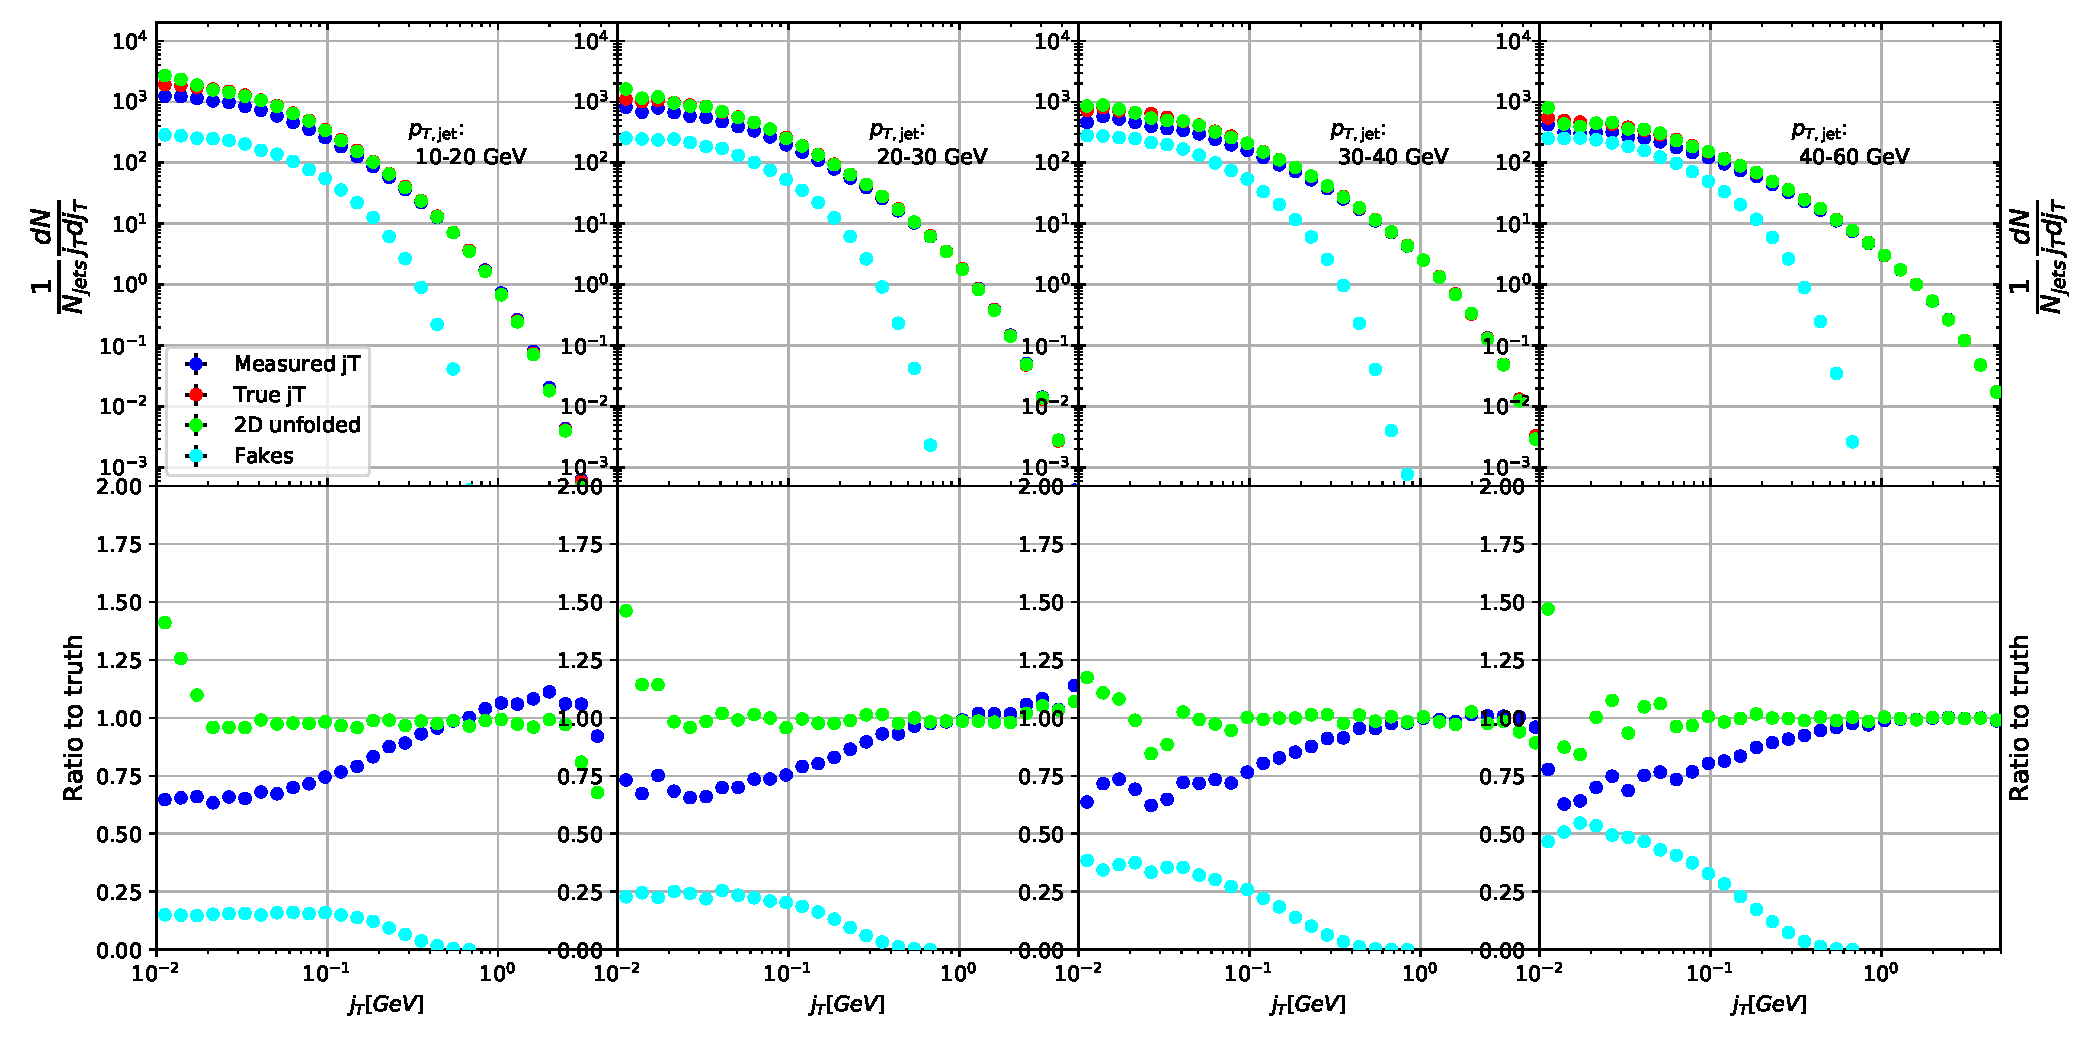
\includegraphics[width=0.9\textwidth]{figures/analysis/ToyMCUnfolder_300k_events.pdf}
\caption{Results from unfolding in Toy Monte Carlo}
\label{fig:toymc}
\end{figure}
\FloatBarrier






\subsubsection{Pythia Response matrices}
A \pythia~6 simulation was carried out to determine the response matrices.  The simulation used the Perugia 2011~\cite{pythiaPerugiaTune} tune with \snn=5.02\tev. The detector response of the particle level tracks was simulated using GEANT3~\cite{Brun:118715,geant}.

Response matrices are filled through correlation between MC detector and particle level jets and tracks. When creating the response matrices detector level tracks in each event are first analysed using the same procedure as for data, but their $\jt{}$ values are stored in an array. This is only done for tracks that are closer than the cone size, $R$, to a jet. Thus most tracks in the event will not have their $\jt{}$ values calculated. The analysis then moves to particle level (MC) tracks. There are analysed similarly, but for each track the code checks whether a corresponding detector level track existed and if that track had a \jt{} value. Finally the code checks for detector level tracks that don't have corresponding particle level track with a \jt{} value.

There are several possibilities that have to be taken into account:
\begin{itemize}
\item We find a corresponding track with a \jt{} value. Response matrix is filled normally with $\left(\jt{}^\mathrm{obs},\pt{,jet}^{obs},\jt{}^\mathrm{true},\pt{,jet}^{true}\right)$
\item We don't find a corresponding track. Record $\left(\jt{}^\mathrm{true},\pt{,jet}^\mathrm{true}\right)$ as a miss 
\item We find a corresponding track, but it didn't have $\jt{}$ value. Most likely because it was not part of a jet in the detector level set. Similary record $\left(\jt{}^\mathrm{true},\pt{,jet}^\mathrm{true}\right)$ as a miss
\item For detector level tracks that have no correspondence in particle level set the code records  $\left(\jt{}^\mathrm{obs},\pt{,jet}^\mathrm{obs}\right)$ as a fake
\end{itemize}

In the analysis code the response matrix is made of an array of 3 dimensional histograms, with $\left(\jt{}^\mathrm{obs},\pt{,jet}^\mathrm{obs},\jt{}^\mathrm{true}\right)$ as axes. The histogram index gives the $\pt{,jet}^\mathrm{true}$ value. The ranges in the response matrices of both $\jt{}$ and $\pt{,jet}$ match the ranges used for the end results. For \jt{} the range is between \unit[0.01]{\gev} and \unit[20]{\gev} and \pt{,jet} between \unit[5]{\gev} and \unit[500]{\gev}.  The ranges are the same in detector and particle level.

As a primary method unfolding is performed with an iterative (bayesian) algorithm using the RooUnfold~\cite{roounfold} package. The number of iterations used is 4.  As a default the true $\jt{}$ distribution from the \pythia~simulation is used as the prior.

%\begin{table}
%\centering
%\caption{$\jt{}$ and $\pt{}$ ranges used in unfolding. The same ranges are used for detector and truth level.}
%\label{tab:unfranges}
%\begin{tabular}{c | c | c}
% & $\jt{}$ & $\pt{,jet}$ \\
% \hline
%Min & 0.01 & 5 \\
%Max & 20 & 500 \\
%\hline
%\end{tabular}
%\end{table}

\subsubsection{Unfolding  closure test}
The \pythia~set is divided into 2 halves. First is used to fill the response matrices, as well as record missed and fake tracks. Second half is used to test the effectiveness of the unfolding method. Jet $\pt{}$ distributions and response matrix are shown in Figure~\ref{fig:ptclosure}. For the range where this analysis is performed, $\unit[40]{\gev} <\pt{,jet} <\unit[150]{\gev}$, the \pt{,jet} distribution is recovered well. At low \pt{,jet} the true distribution can't be recovered. The primary reason is that jet with $\pt{,obs}<\unit[5]{\gev}$ are not considered, although $\pt{,true}$ would have been above $\unit[5]{\gev}$. Thus these are missing from the response matrix and their contribution can't be unfolded. At high $\pt{,jet}$ the situation is opposite. Jets with $\pt{,true} > \unit[500]{\gev}$ are lost due to histogram limits. Thus jets just below this limit are overrepresented in the response matrix for $\pt{,obs}\approx \unit[500]{\gev}$. 
 
 \begin{figure}
\begin{subfigure}[b]{0.5\textwidth}
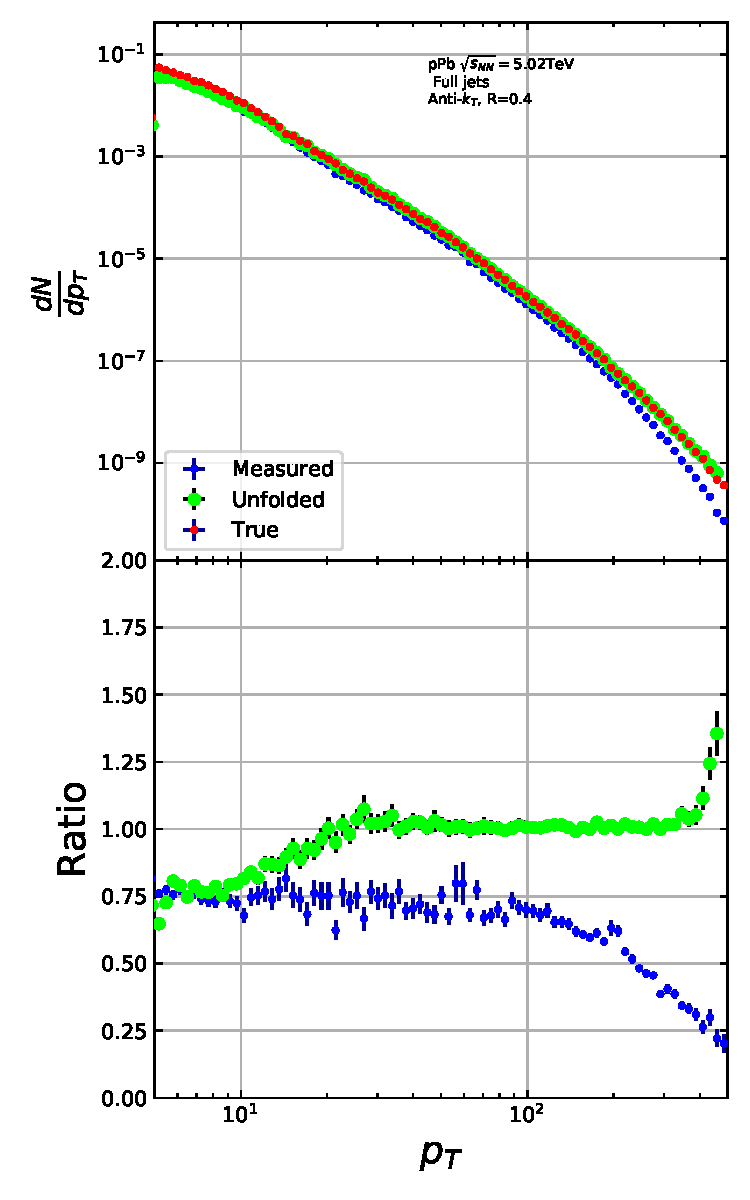
\includegraphics[width=0.7\textwidth]{figures/analysis/JetPtUnfolded.pdf}
%\caption{Unfolded jet $\pt{}$ distribution in \pythia~closure test}
%\label{fig:jetptunf}
\end{subfigure}
\begin{subfigure}[b]{0.5\textwidth}
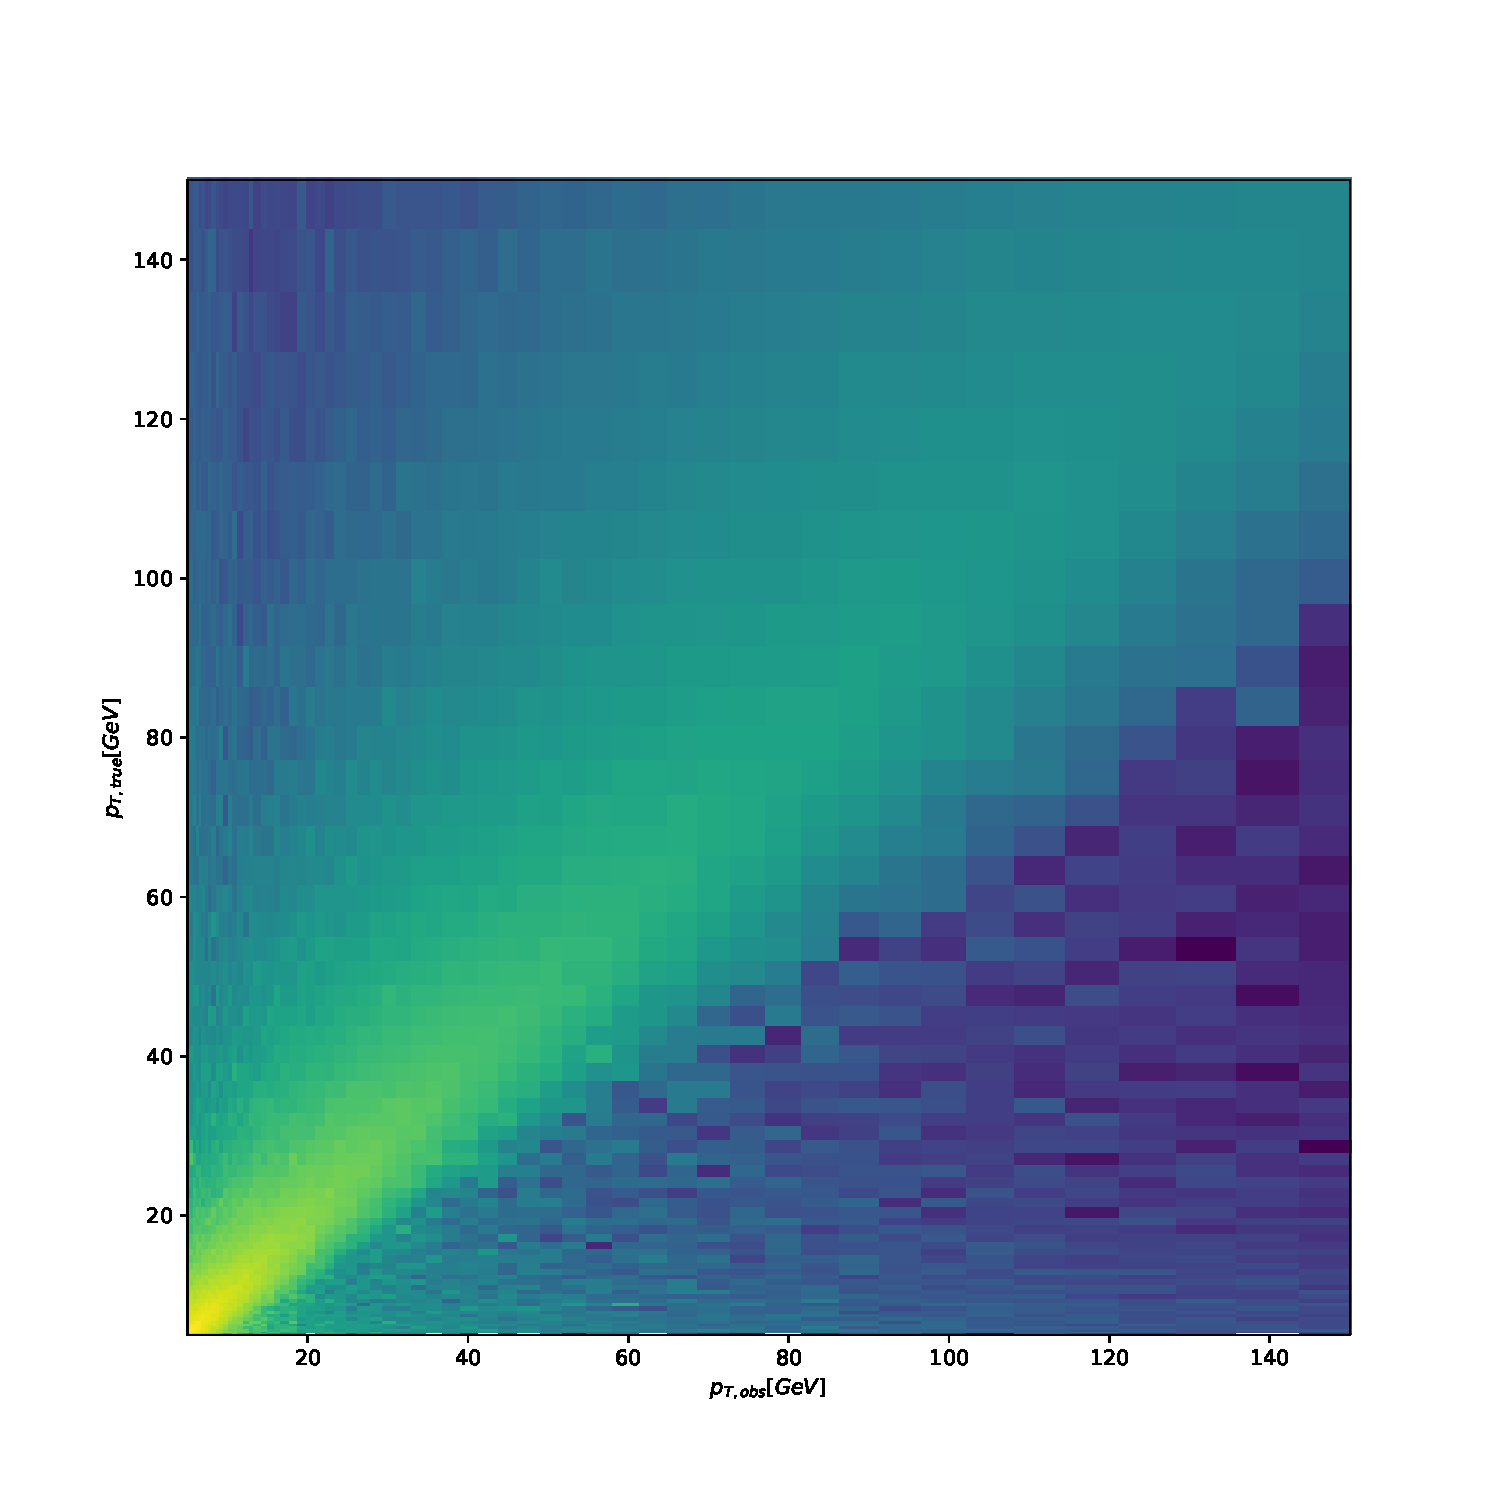
\includegraphics[width=0.8\textwidth]{figures/analysis/JetPtResponse.pdf} 
%\caption{Jet $\pt{}$ response matrix from unfolding closure test}
%\label{fig:jetptresponse}
\end{subfigure}
\caption{\emph{left:} Unfolded jet $\pt{}$ distribution in \pythia~closure test \emph{right:} Jet $\pt{}$ response matrix from unfolding closure test}
\label{fig:jetptclosure}
\end{figure}
 
Response matrices within single jet $\pt{}$ bins are shown in Figure~\ref{fig:response}. Results from the closure test are shown in Figure~\ref{fig:closure}. In the lowest jet $\pt{}$ bins unfolding fails to recover the true distribution. The lowest jet $\pt{}$ bins are dominated by combinatorial jets and thus the true detector response is likely not retrieved.

Above $\unit[30]{\gev} <\pt{,jet} < \unit[40]{\gev}$~the distribution is recovered well in the mid $\jt{}$ region. At $\jt{} < \unit[0.1]{\gev}$ there is clear discrepancy and hence the final results are shown only for $\jt{} > \unit[0.1]{\gev}$. Additionally there is some discrepancy at very high $\jt{}$. This is taken into account in the unfolding systematics. %{\color{red}(TODO: Show this) }
\begin{figure}
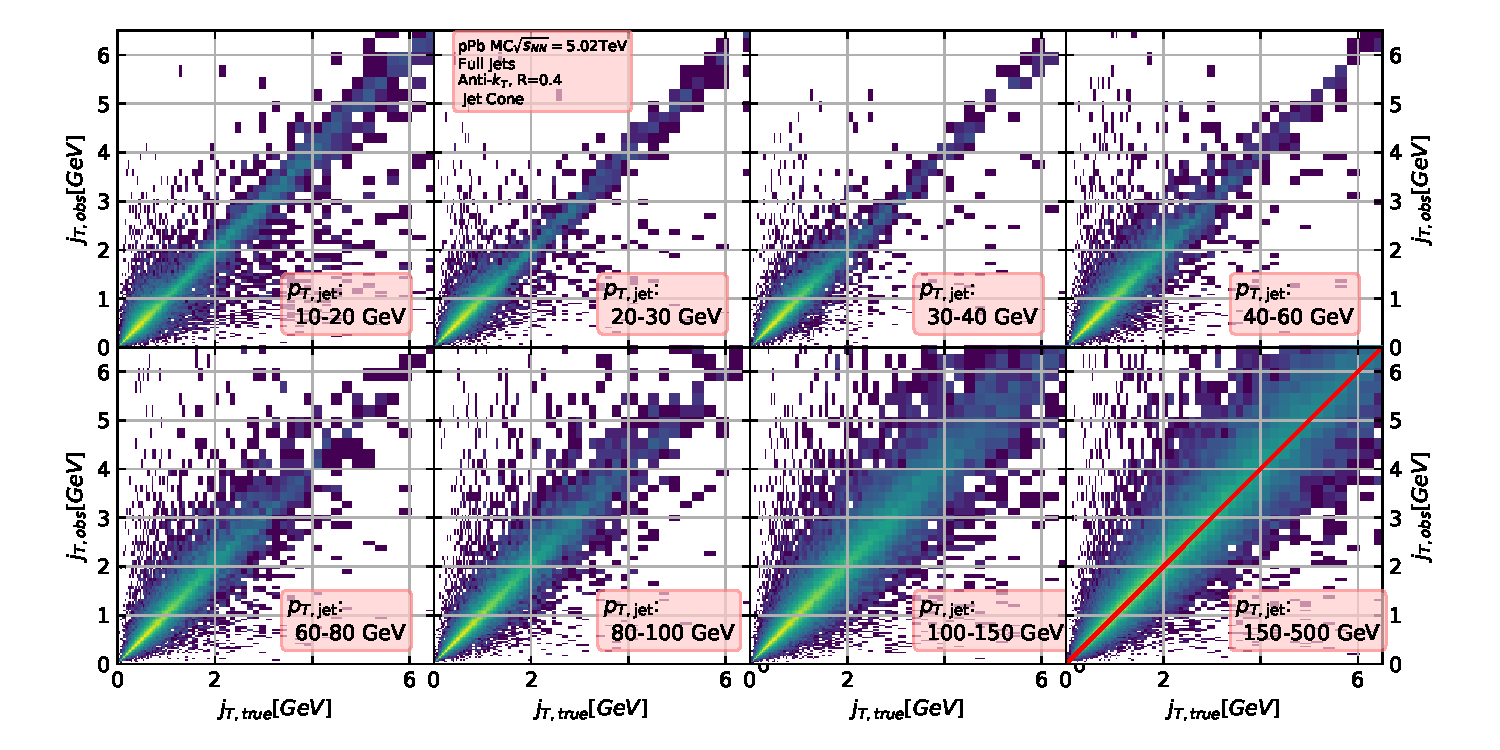
\includegraphics[width=0.99\textwidth]{figures/analysis/ResponseMatrixNFin00.pdf}
\caption{$\jt{}$ Response matrices in individual $\pt{,jet}$ bins}
\label{fig:response}
\end{figure}

\begin{figure}
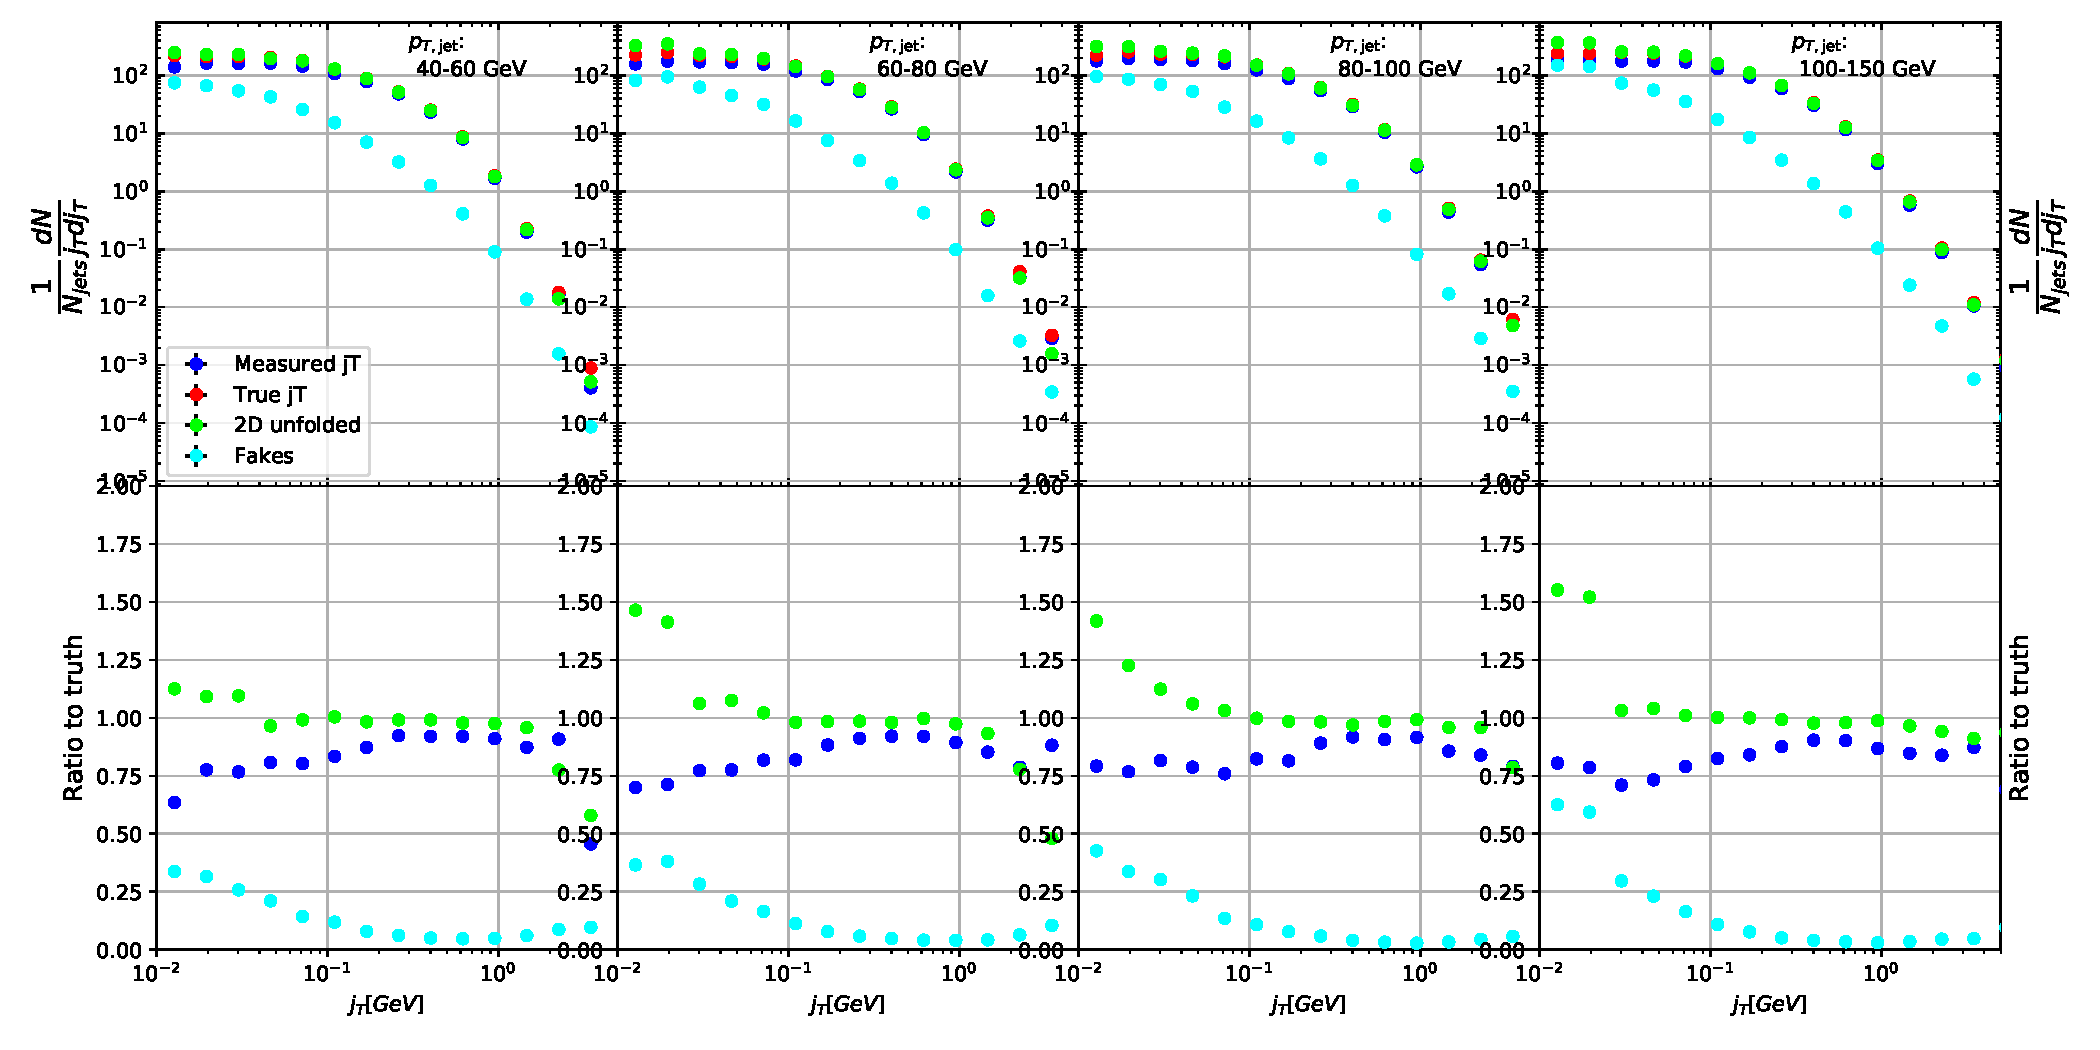
\includegraphics[width=0.99\textwidth]{figures/analysis/PythiaTest.pdf}
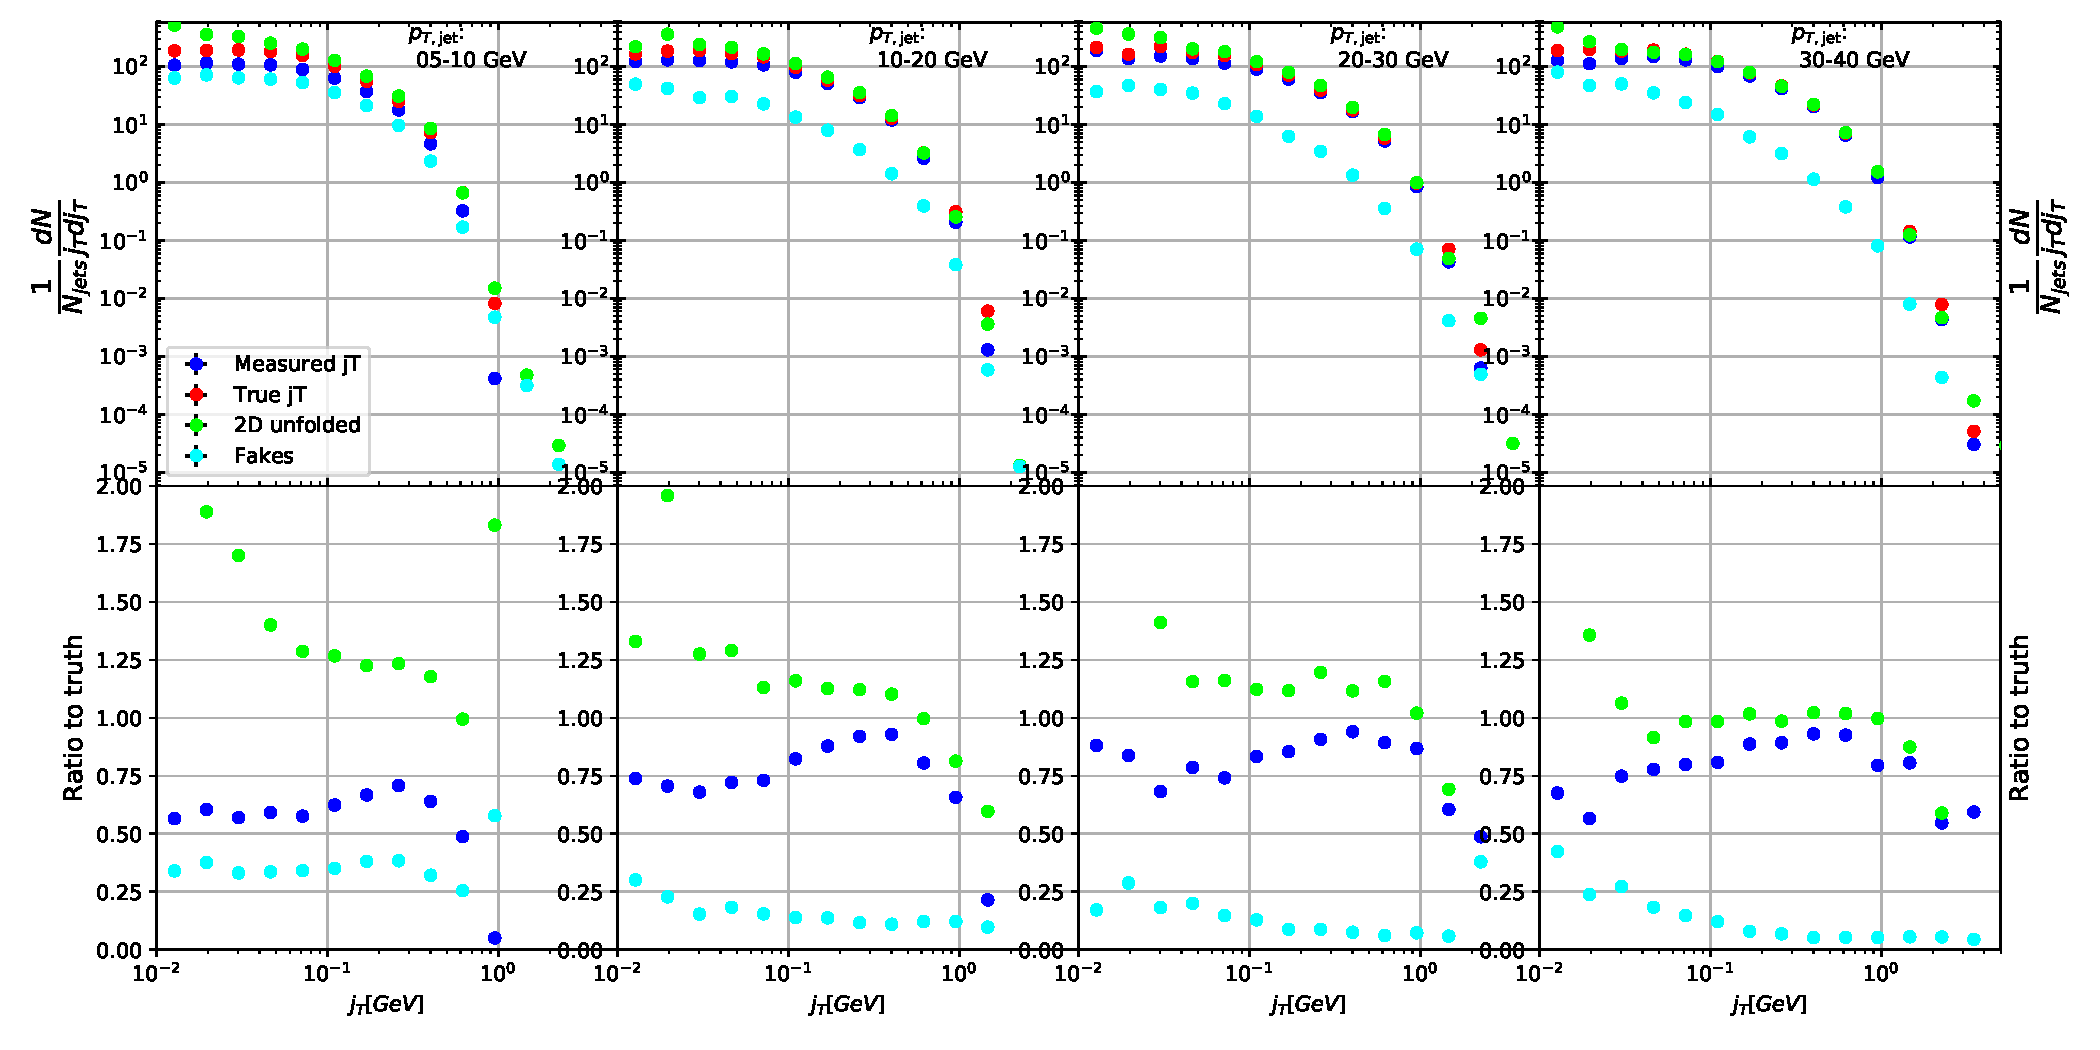
\includegraphics[width=0.99\textwidth]{figures/analysis/PythiaTest_Extra.pdf}
\caption{Pythia closure test results. Fake tracks include also tracks that do exist in the true dataset, but for one reason or another were not given $\jt{}$ values. $\jt{}$ is only calculated for tracks that are associated with jets.}
\label{fig:closure}
\end{figure}


\FloatBarrier


 
\subsection{Background}
\label{sec:bg}
When calculating \jt{} distributions for jet constituents there is a contribution from the underlying event (UE), i.e. tracks that just happen to be close to the jet axis.
To find the signal coming from the actual jet we need to subtract the background (UE) contribution. On a jet-by-jet basis this is difficult to achieve reliably, so one must estimate the background contribution in the inclusive  distribution. A schematic view of the background contribution is shown in Figure~\ref{fig:bgdef}. 

We have two methods for background estimation. In the first we look at the direction perpendicular to the jet. This is assumed to be the region least likely to contain jet contributions. In the second method we randomly assign the tracks of event new $\phi$ and $\eta$ values. The result is thus guaranteed to be uncorrelated.

\begin{figure}[h]
\centering
\begin{subfigure}{0.4\textwidth}
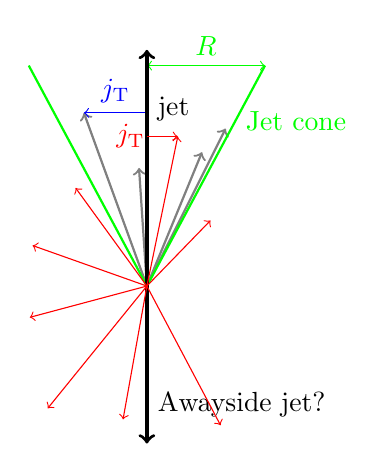
\begin{tikzpicture}
\draw[gray, thick, ->] (0,0) -- (1,2);
\draw[gray, thick, ->] (0,0) -- (-0.8,2.2);
\draw[gray, thick, ->] (0,0) -- (-0.1,1.5);
\draw[gray, thick, ->] (0,0) -- (0.7,1.7);
\draw[green, thick] (0,0) -- node[near end, right] {Jet cone}(1.5,2.8);
\draw[green, thin, <->] (0,2.8) -- node[midway, above] {$R$} (1.5,2.8);
\draw[green, thick] (0,0) --  (-1.5,2.8);
\draw[blue, thin, ->] (0,2.2) -- node [midway, above] {\jt{}} (-0.8,2.2);
\draw[black, very thick, ->] (0,0) -- node [near end,right] {jet} (0,3);
\draw[black, very thick, ->] (0,0) -- node [near end, right] {Awayside jet?} (0,-2);
\draw[red, thin, ->] (0,0) -- (-1.25982281336992,-1.55333398820495);
\draw[red, thin, ->] (0,0) -- (-1.45147226001971,0.514614689251372);
\draw[red, thin, ->] (0,0) -- (-0.30285006631157,-1.69312782663775);
\draw[red, thin, ->] (0,0) -- (0.8074529522207,0.832838357636147);
\draw[red, thin, ->] (0,0) -- (-1.48782136581293,-0.397476519344932);
\draw[red, thin, ->] (0,0) -- (0.935437036685518,-1.76775494636474);
\draw[red, thin, ->] (0,0) -- (-0.905166754522554,1.2459025429411);
\draw[red, thin, ->] (0,0) -- (0.392170769946368,1.89994791697027);
\draw[red, thin, ->] (0,1.89994791697027) -- node [near start, left] {\jt{}} (0.392170769946368,1.89994791697027);
\end{tikzpicture}

\caption{Orange is underlying event while gray tracks represent the signal}
\end{subfigure}
\begin{subfigure}{0.4\textwidth}
\documentclass[border=5mm]{standalone}
\usepackage{tikz}
\usetikzlibrary{positioning}
\usepackage{xcolor}
\usetikzlibrary{shapes,arrows}
\usetikzlibrary{trees}
\usetikzlibrary{shadows.blur}
\usetikzlibrary{decorations.pathmorphing}
\usetikzlibrary{decorations.markings}
\usetikzlibrary{intersections, calc}
\def\jt#1{\ensuremath{j_{\rm T#1}}}
\begin{document}
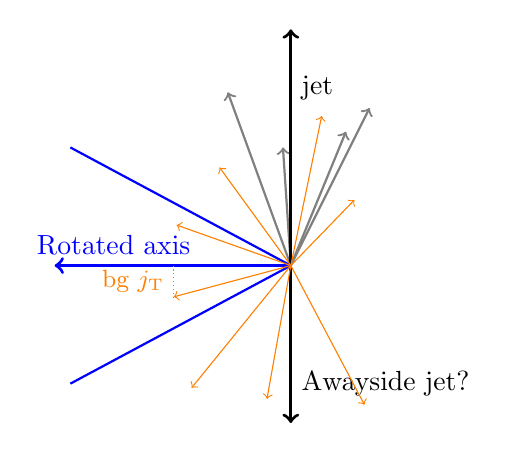
\begin{tikzpicture}
\draw[gray, thick, ->] (0,0) -- (1,2);
\draw[gray, thick, ->] (0,0) -- (-0.8,2.2);
\draw[gray, thick, ->] (0,0) -- (-0.1,1.5);
\draw[gray, thick, ->] (0,0) -- (0.7,1.7);
\draw[blue, thick] (0,0) -- (-2.8,1.5);
\draw[blue, thick] (0,0) --  (-2.8,-1.5);
\draw[blue, very thick, ->] (0,0) -- node [near end, above] {Rotated axis} (-3,0);
\draw[black, very thick, ->] (0,0) -- node [near end,right] {jet} (0,3);
\draw[black, very thick, ->] (0,0) -- node [near end, right] {Awayside jet?} (0,-2);
\draw[orange, thin, ->] (0,0) -- (-1.25982281336992,-1.55333398820495);
\draw[orange, thin, ->] (0,0) -- (-1.45147226001971,0.514614689251372);
\draw[orange, thin, ->] (0,0) -- (-0.30285006631157,-1.69312782663775);
\draw[orange, thin, ->] (0,0) -- (0.8074529522207,0.832838357636147);
\draw[orange, thin, ->] (0,0) -- (-1.48782136581293,-0.397476519344932);
\draw[orange, thin, ->] (0,0) -- (0.935437036685518,-1.76775494636474);
\draw[orange, thin, ->] (0,0) -- (-0.905166754522554,1.2459025429411);
\draw[orange, thin, ->] (0,0) -- (0.392170769946368,1.89994791697027);
\draw[orange, thin, densely dotted] (-1.48782136581293,0) -- node [midway, left] {\small bg $\jt{}$} (-1.48782136581293,-0.397476519344932);
\end{tikzpicture}
\end{document}

\caption{We estimate the background using a cone where the axis is perpendicular to the jet axis}
\end{subfigure}
\caption{Background estimation}
\label{fig:bgdef}
\end{figure}

\subsubsection{Perpendicular cone background}
As a primary method to estimate the background we look at regions of the detector where there are no tracks from jets, but only uncorrelated tracks from the underlying event. The underlying event is thus estimated by looking at an imaginary jet cone perpendicular to the observed jet axis ($\frac{\pi}{2}$ Rotation in $\phi$). 

%$\jt{}$ is calculated for any tracks found within this cone. The vector sum of the individual track momentum and the imaginary jet axis is used as reference for $\jt{}$. The background obtained in this manner is subtracted from the unfolded inclusive $\jt{}$ distribution, which gives the resulting signal distribution. To make sure there is no jet contribution in the background, any events with jets inside the perpendicular cone are not used for background estimation.

After calculating the $\jt{}$ values for tracks in the jet, we rotate the jet axis by $\frac{\pi}{2}$ in positive $\phi$ direction. We check that there are no other jets closer than $2R$ to the rotated axis. Otherwise background calculation is skipped for this jet. Probability of this happening is 1-2\% depending on the jet $\pt{}$ bin.

If we don't find other jets in the vicinity we move on to estimate the background. We find all tracks within a cone of radius $R$ around the rotated axis and calculate $\jt{}$ of these tracks with respect to the rotated axis. %Auto-correlations are discussed in Section~\ref{sec:autoC}. 

This background procedure is a part of the reason for using charged tracks inside a fixed size cone, instead of jet constituents. To be representative of the actual underlying event contribution the size and shape of the background estimation region should match the area where $\jt{}$ is calculated. The irregular shape of a jet would be hard to take into account when calculating background. Thus the regions are made to match by considering fixed size cones for $\jt{}$.






\begin{figure}[tb]
\centering
\tikzstyle{decision} = [diamond, draw, fill=blue!20, 
    text width=4.5em, text badly centered, node distance=3cm, inner sep=0pt]
\tikzstyle{block} = [rectangle, draw, fill=blue!20, 
    text width=5em, text centered, rounded corners, minimum height=4em]
\tikzstyle{line} = [draw, -latex',orange]
\tikzstyle{cloud} = [draw, ellipse,fill=red!20, node distance=3cm,
    minimum height=2em]
    
\tiny 
\begin{tikzpicture}[node distance = 1cm, auto]
    % Place nodes
    \node [block] (init) {Jet found};
    \node [block, below of=init, node distance = 2cm] (rotate) {Rotate jet axis by $\pi/2$ (positive $\phi$)};
    \node [decision, below of=rotate, node distance = 2.5cm](jets){Other jets close to the rotated axis? ($<2R$)};
    \node [block, left of=jets, node distance = 2.5cm] (discard) {Don't calculate background};
    \node [block, right of=jets, node distance = 2.5cm] (tracks) {Find tracks within cone R};
    \node [block, above of=tracks, node distance = 2cm](sum) {Calculate vector sum of track and rotated axis};
    \node [block, right of =sum, node distance = 2cm](jt) {Calculate $\jt{}$ with respect to the vector sum};
    
    % Draw edges
    \path [line] (init) -- (rotate);
    \path [line] (rotate) -- (jets);
    \path [line] (jets) -- node [near start] {yes} (discard);
    \path [line] (jets) -- node [near start] {no} (tracks);
    \path [line] (tracks) -- node [near start] {For each track} (sum);
    \path [line] (sum) -- (jt);
    \path [line] (jt) |- (tracks);
    
\end{tikzpicture}

\caption{Flowchart representation of the perpendicular cone background procedure}
\label{fig:bgflow}
\end{figure}


One additional consideration is the issue of auto-correlations as the jet axis is simply a vector sum of all its constituents. Thus having an additional track in the jet from the underlying event moves the jet axis towards this track. Since the axis is now closer to the track, it has a smaller $\jt{}$ value. Assuming a \unit[1]{\gev} background track  at the edge of a $R = 0.4$ cone the $\jt{}$ value would be \unit[0.4]{\gev}. If this is added to a  \unit[5]{\gev} jet, the $\jt{}$ value becomes \unit[0.33]{\gev} after the jet axis moves. In a \unit[50]{\gev} jet it would be \unit[0.39]{\gev}. This is a region where the inclusive $\jt{}$ distribution is dominated by background. The distribution is also steeply falling. Overestimating the background can lead to a situation where the background estimation exceeds the inclusive distribution.

%\begin{figure}[htp]
%\centering
%\begin{subfigure}{0.99\textwidth}
%\includegraphics[width=0.95\textwidth]{pics/jt_in_jet_bg}
%\caption{Illustration of the effect of a track from the underlying event in a jet and for a fixed background axis}
%\end{subfigure}
%\begin{subfigure}{0.45\textwidth}
%\includegraphics[width=0.95\textwidth]{pics/jt_correction}
%\caption{Background behavior after adding auto-correlations}
%\end{subfigure}
%\caption{Auto-correlations in background and jets}
%\end{figure}

To take this effect into account we can't use a fixed axis for background, but it has to behave like a jet would when additional tracks are added. Thus before calculating $\jt{}$ values we make a vector sum of the track and the axis used for background, which is either the perpendicular cone axis or the random axis depending on the background method. In each case the momentum of this background axis is assumed to be the same as the jet which initiated the background estimation.

In \pPb data there is on average about one underlying event track in a $R = 0.4$ cone. If there would be more, one should consider taking the vector sum of all tracks inside the cone. As there is usually only one track and if there are more it's unlikely that more than one has high momentum, taking the vector sum track-by-track should be enough.








%\begin{figure}[htp]
%\centering
%\includegraphics[width=0.75\textwidth]{pics/jt_back}\\
%\end{figure}


%\begin{figure}[htp]
%\includegraphics[width=0.85\textwidth]{pics/2014-May-16-p-pb_jt_bgsub_060-080_0005-0100} \\
%\line(1,0){250}\\
%\raggedright
%\tiny{Král, Jiří, \textit{ Intrinsic Transverse Momentum Distribution of Jet
%Constituents in P-Pb Collisions at ALICE}, Ph.D. Thesis, University of Jyväskylä, 2014}
%%\item jT distribution is constructed from charged jet constituents
%\end{figure}

\subsubsection{Random background}
In the random background method we look at all tracks in the event, except for tracks close to jets found by the jet algorithm. We randomly assign new $\eta$ and $\phi$ values to all tracks using uniform distributions with $\left|\eta\right| < 1.0$. $\pt{}$ values are kept the same. To increase statistics there is a possibility to create a number of random tracks for each actual track. In the analysis we do this 10 times for each track. Again the track $\pt{}$ value is kept the same. 

We create a random jet cone from uniform $\eta$ and $\phi$ distributions. Here $\left| \eta \right| < 0.25$. Now we calculate $\jt{}$ of the random tracks with respect to the random cone axis. As in the perpendicular cone method auto-correlations are added before calculating \jt{}.

Comparison between perpendicular cone and random background in Figure~\ref{fig:bgcomparison}. The advantage of the random background method is that the procedure can be repeated several times for each event, which allows producing additional statistics. However, it seems that, especially in the highest $\pt{,jet}$ bins there is some jet contribution left at the high end. Naturally there is no correlation between the tracks and the background axis, but if some high momentum tracks originating from jets were not subtracted and happen to hit the edge of the background cone, they can increase the high $\jt{}$ yield in the background estimation.

\begin{figure}[htb]
\centering
\begin{subfigure}{0.95\textwidth}
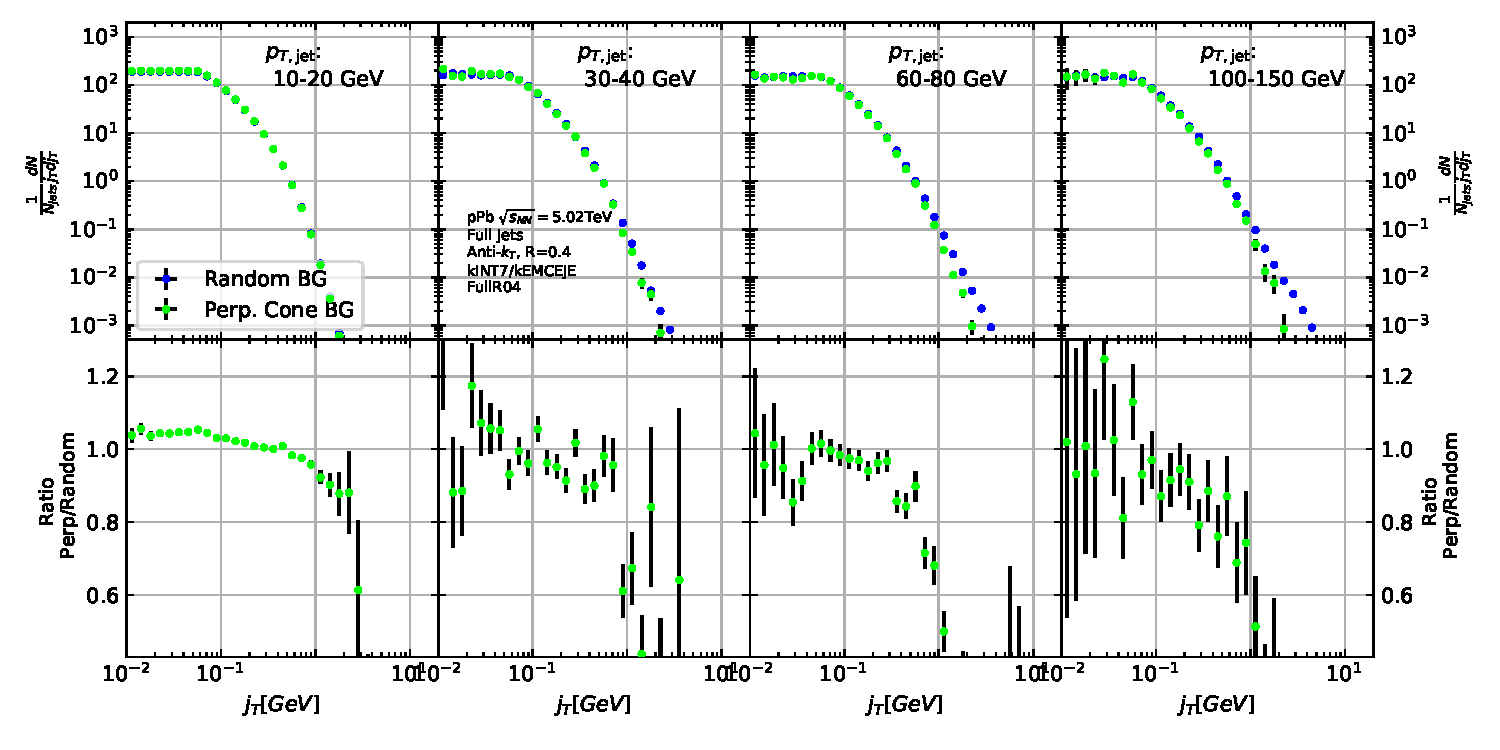
\includegraphics[width=\textwidth]{results/MixedFullJetsR04BackgroundComparison.pdf}
%Tag 20170810 python2.7 Python/InclusiveWithBackground.py legotrain_CF_pPb-1053_20170223-2002_LHC13bcde.root
\end{subfigure}
\caption{$\jt{}$ background with two different methods}
\label{fig:bgcomparison}
\end{figure}

We observe that the results from perpendicular cone background show no observable change between $\pt{,jet}$ bins. It is a good indication that the background is actually dominated by the underlying event over the entire $\jt{}$ region. 

Thus as a primary method of background estimation the perpendicular cone method is used. The random background method is used to estimate systematic contributions by comparing the final results obtained with this method to the results obtained from the perpendicular cone method.


\FloatBarrier
 \subsection{Fitting}
 \label{sec:fitting}
After unfolding and background subtraction the resulting signal distributions are fitted with a 2 component function shown in Eq.~\ref{eq:fit}. Gaussian distribution is used for low $\jt{}$ and an inverse gamma function is used for high $\jt{}$. The Gaussian is taken to have the center at $\jt{} = 0$. In total this gives 5 parameters. The fitting procedure was inspired by the dihadron $\jt{}$ analysis by ALICE~\cite{ALICEjt}. The complete fitting function is 

\begin{equation}
\frac{1}{N_{\mathrm{jets}}}\frac{\mathrm{d}N}{\jt{} \mathrm{d}\jt{}} = \frac{B_2}{B_1\sqrt{2\pi}}e^{-\frac{\jt{}^2}{2B_1^2}}+\frac{B_3B_5^{B_4}}{\Gamma\left(B_4\right)}\frac{e^{-\frac{B_5}{\jt{}}}}{\jt{}^{B_4+1}}.
\label{eq:fit}
\end{equation}

To achieve stable results the fitting is performed in two steps. First both components are fitted separately. Gaussian component is fitted to the low end of $\jt{}$. Inverse gamma component is fitted to $\jt{}$ above $\unit[1]{\gevc}$. After getting the results from the individual fits they are combined into a single function with initial values from the individual results and an additional fit is performed. 
%Fitting only the Gaussian component to the entire distribution produces approximately the same result as the Gaussian component in the two-component model.

After getting the fit function $\sqrt{\left<\jt{}^2\right>}$ (RMS) and yield values are extracted separately from each component. The narrow component RMS is

\begin{equation}
\sqrt{\left<\jt{}^2\right>}=\sqrt{2}B_1,
\end{equation}


\noindent and the wide component RMS value is calculated as 

\begin{equation}
\sqrt{\left<\jt{}^2\right>}=\frac{B_5}{\sqrt{\left(B_4-2\right)\left(B_4-3\right)}},
\end{equation}


\noindent where it is required that $B_4 > 3$.

The statistical errors can be calculated with the general error propagation formulas. As a result one gets errors for the narrow component RMS
\nobreak
\begin{equation}
\delta \sqrt{\left<\jt{}^2\right>} = \sqrt{2}\delta B_1
\end{equation}
\noindent and for the wide component RMS

\begin{equation}
\delta \sqrt{\left<\jt{}^2\right>} = \sqrt{ \left( \frac{\left(5-2 B_4 \right) B_5 \delta  B_4}{\left( 2\left(  B_4-2\right)\left( B_4-3\right)      \right)^{\frac{3}{2}}}\right)^2 + \left( \frac{\delta B_5}{\sqrt{\left( B_4-2\right)\left( B_4-3\right)}}      \right)^2  }.
\end{equation}

%Yield(narrow)
%$$\frac{\delta Y}{N_{\mathrm{jet}}} = \sqrt{\frac{B_2^2\delta B_1^2+B_1^2\delta B_2^2}{2\pi}}$$
% Yield(Wide)
% $$ \frac{\delta Y}{N_{\mathrm{jet}}} = \sqrt{\left(\frac{B_5\delta B_3}{B_4-1} \right)^2+ \left(\frac{B_3B_5\delta B_4}{\left(B_4-1 \right)^2} \right)^2 + \left(\frac{B_3 \delta B_5}{B_4-1}\right)^2}$$



% !TEX root = thesis.tex

\section{TPC Upgrade?}
\label{sec:tpc}
% !TEX root = thesis.tex
\section{Systematic erros}
{\color{red} Extend Systematics}
\label{sec:systematicerrors}
The main systematic uncertainties in this analysis come from the background estimation, the unfolding procedure and uncertainty in the tracking efficiency. Tracking uncertainties are estimated from variations of the track selection cuts defined in Sec.~\ref{sec:experimentaldetails}. 

%The resulting variations in RMS are shown in Table \ref{tab:systematics}. The uncertainties from unfolding and background subtraction are of the same magnitude. 

The systematics in background estimation were studied using an alternative method to extract the background, mainly the random background method. The resulting uncertainty is below 5\% for the wide component RMS and below 9\% for the narrow component RMS. 

The systematic uncertainty that arises from the unfolding procedure is estimated by performing the unfolding with two separate methods. Data corrected by the iterative unfolding method are used as the results and the SVD unfolding method is employed to estimate the uncertainty. In a \textsc{Pythia} closure test the true distribution was in general found to be between the unfolded distributions from the iterative and SVD method. The difference between the methods when unfolding data should give a reasonable estimate of the unfolding uncertainty. The resulting uncertainty is below 8\% for both wide and narrow component RMS.



\begin{table}[htb]
\centering
\caption{Summary of systematic errors}
\label{tab:systematics}
\begin{tabular}{ l | c | r }
  Systematic & Wide RMS & Narrow RMS \\
    \hline			
  Background & 5 \% & 9 \% \\
  Unfolding & 8 \% & 8 \% \\
  Tracking & ? \% & ? \% \\
  Total & 9 \% & 12\% \\
  \hline
  \end{tabular}
  \end{table}
  
 \subsection{Background}
The uncertainty coming from background estimation is estimated by subtracting the background separately for the perpendicular cone and random background methods. Comparisons of the resulting signal distributions are shown in Fig.~\ref{fig:signal}. 
 
 \begin{figure}[htb]
\centering
\begin{subfigure}{0.95\textwidth}
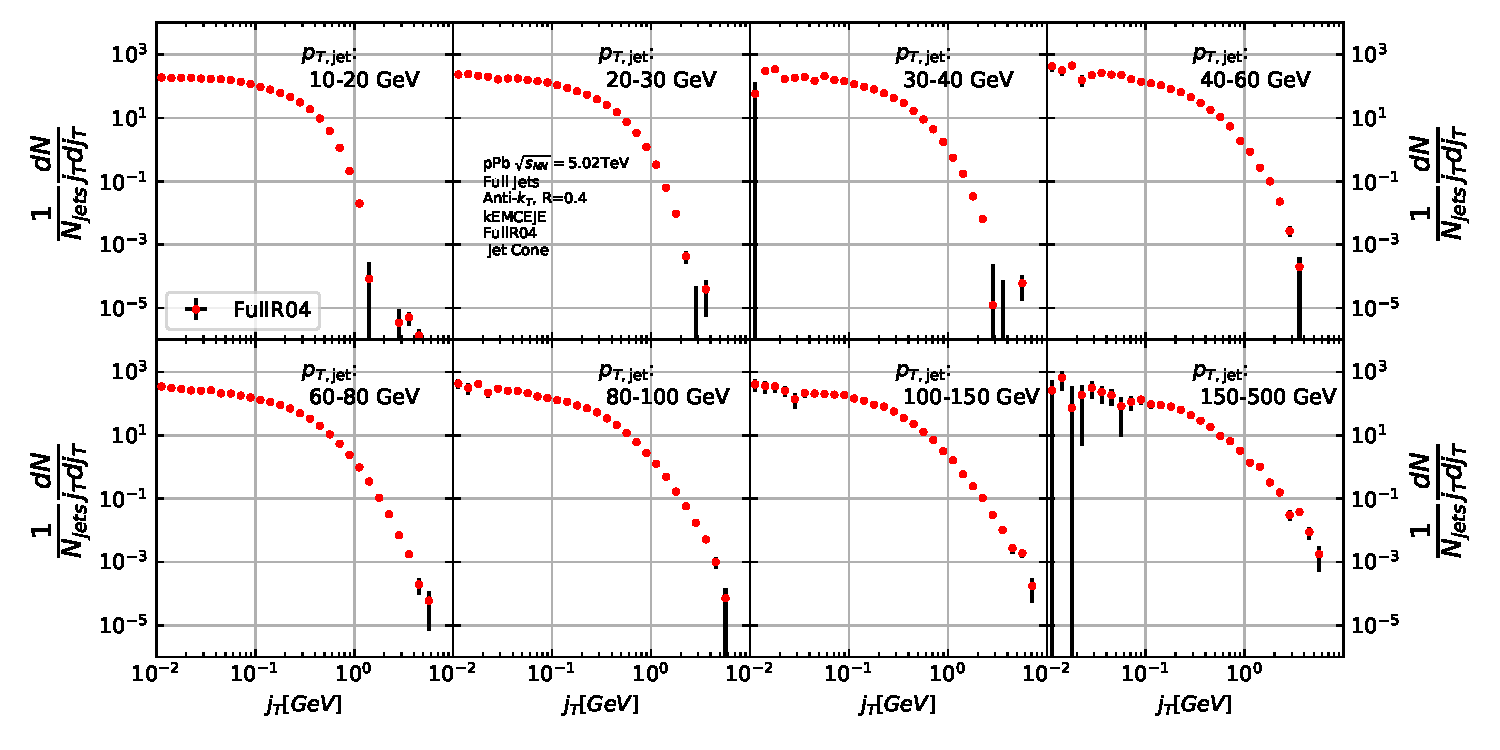
\includegraphics[width=\textwidth]{results/MixedFullJetsR04JetConeJtSignal.pdf}
%Tag 20170810 python2.7 Python/DrawSignal.py legotrain_CF_pPb-1053_20170223-2002_LHC13bcde.root
\end{subfigure}
\caption{$\jt{}$ signal with background subtracted}
\label{fig:signal}
\end{figure}

 
Fits are then performed on both perpendicular cone and random background signals. Difference between them is taken as the systematic error. The fits for individual bins from the random background method are shown in figure \ref{fig:fitsrandombg}. Resulting differences between the methods for different components are shown in figure \ref{fig:systbg}. The dotted lines are put at $\pm \unit[5]{\%}$ for the narrow component and at $\pm \unit[8]{\%}$ for the wide component. These are taken as systematic estimates for the entire $\pt{jet}$ range.

\begin{figure}[htb]
\centering
\begin{subfigure}{0.95\textwidth}
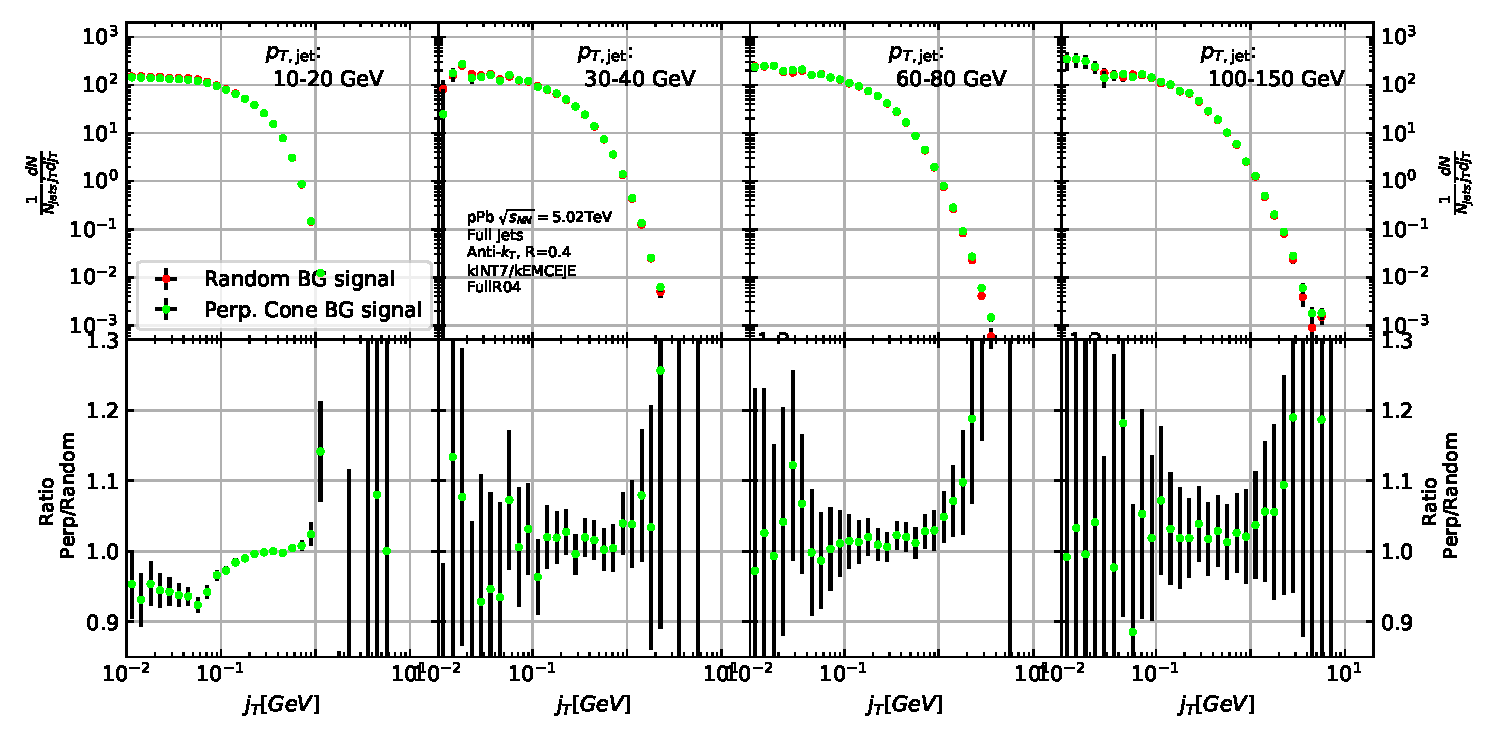
\includegraphics[width=\textwidth]{results/MixedFullJetsR04SignalBackgroundComparison.pdf}
%Tag 20170810 python2.7 Python/DrawSignal.py legotrain_CF_pPb-1053_20170223-2002_LHC13bcde.root
\end{subfigure}
\caption{Comparison of the effect of background method on $\jt{}$ signal.}
\label{fig:signalbg}
\end{figure}


\begin{figure}
\centering
\begin{subfigure}{0.24\textwidth}
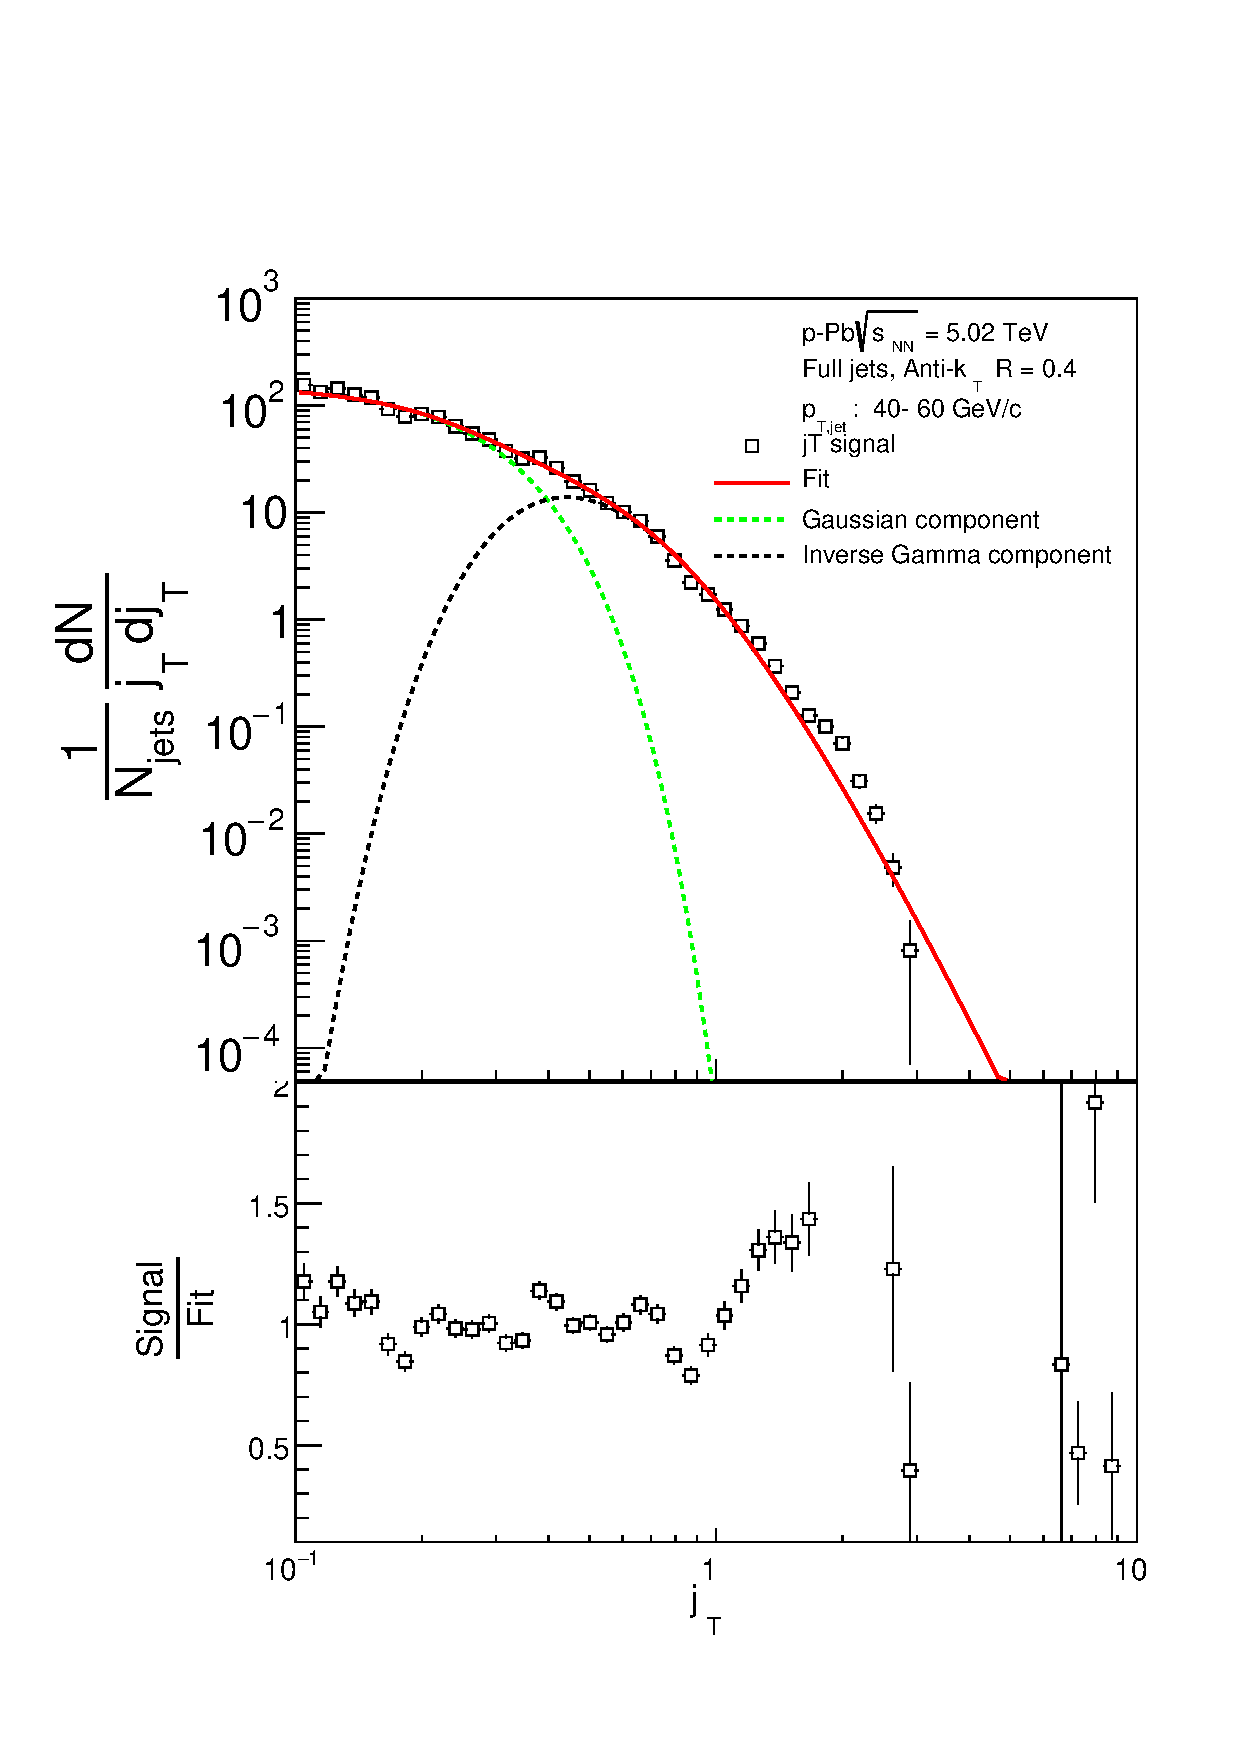
\includegraphics[width=0.95\textwidth]{results/JetConejTSignalFit/JetConejTSignalFitNFin00JetPt04randomBgBayes}
\end{subfigure}
\begin{subfigure}{0.24\textwidth}
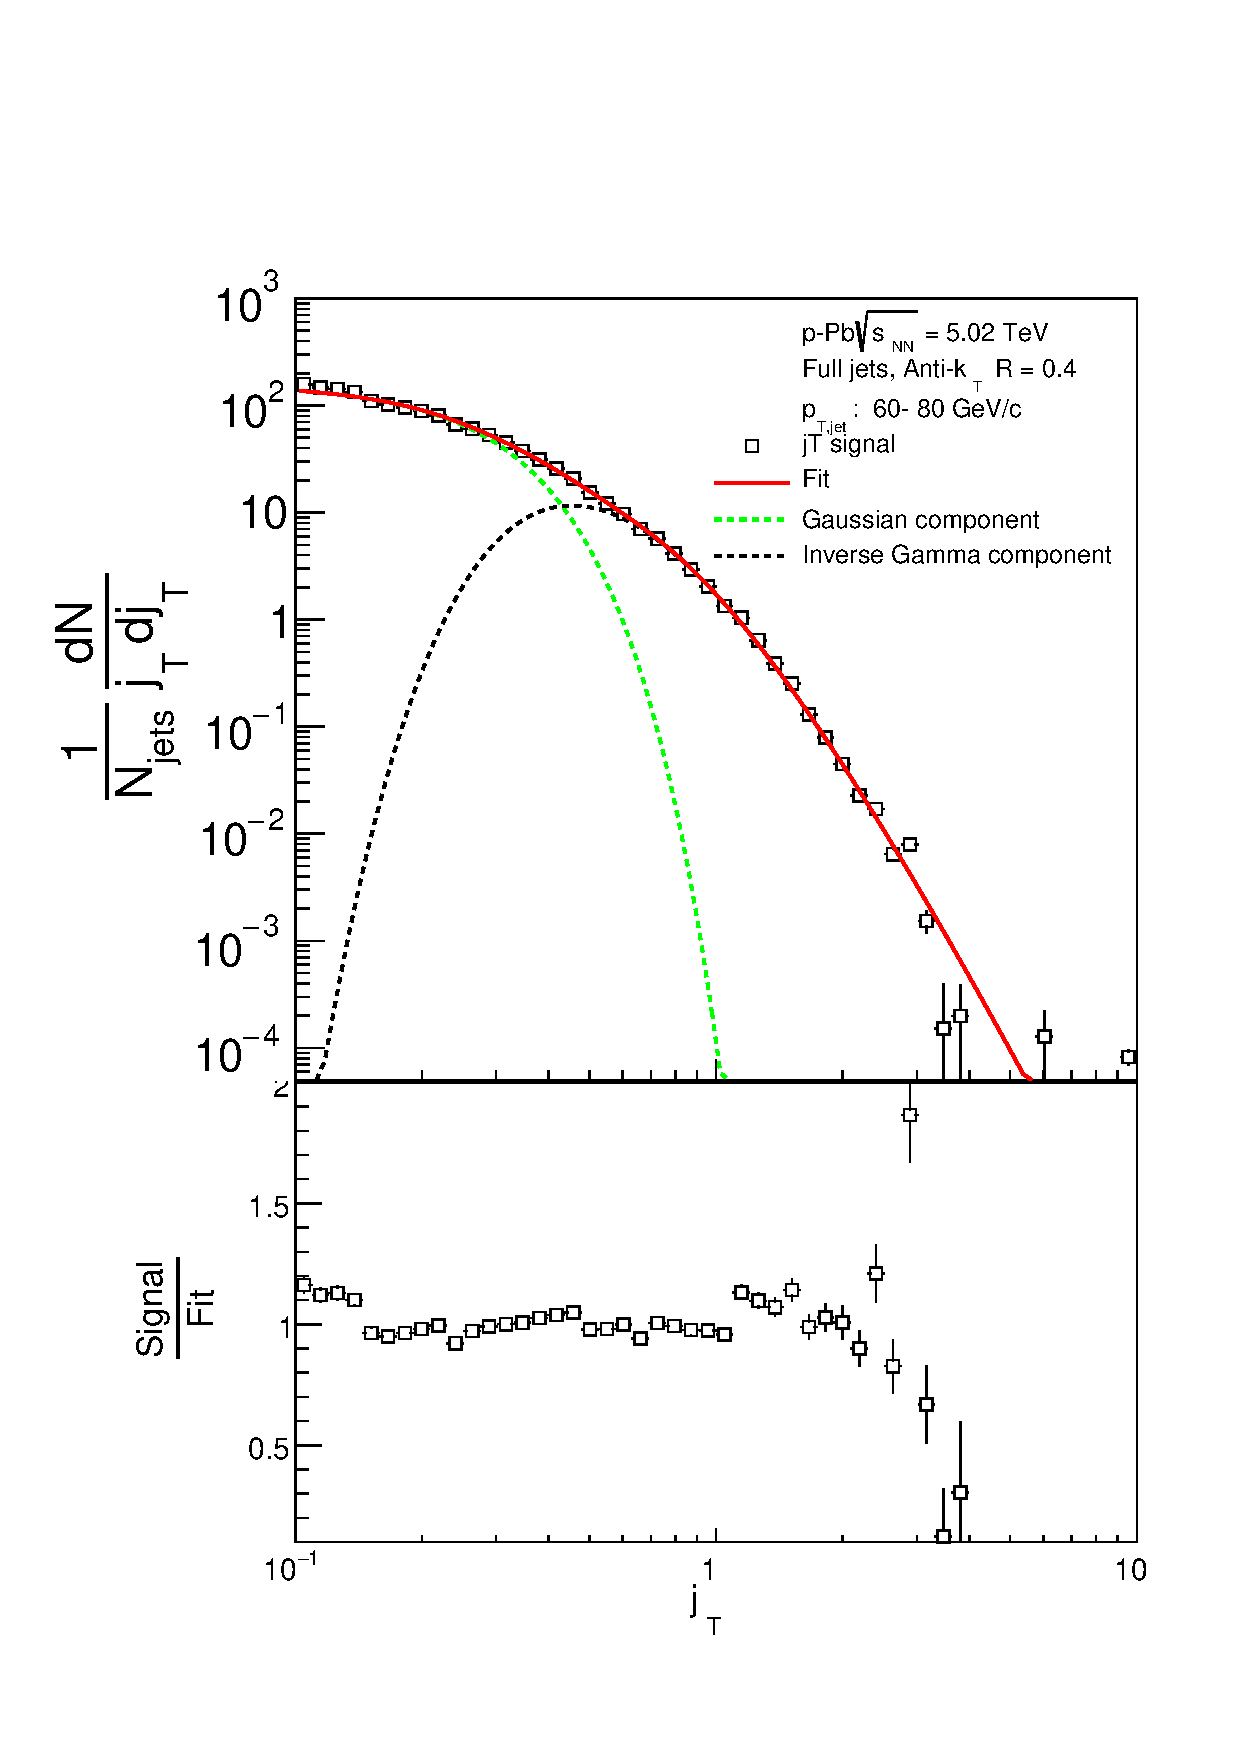
\includegraphics[width=0.95\textwidth]{results/JetConejTSignalFit/JetConejTSignalFitNFin00JetPt05randomBgBayes}
\end{subfigure}
\begin{subfigure}{0.24\textwidth}
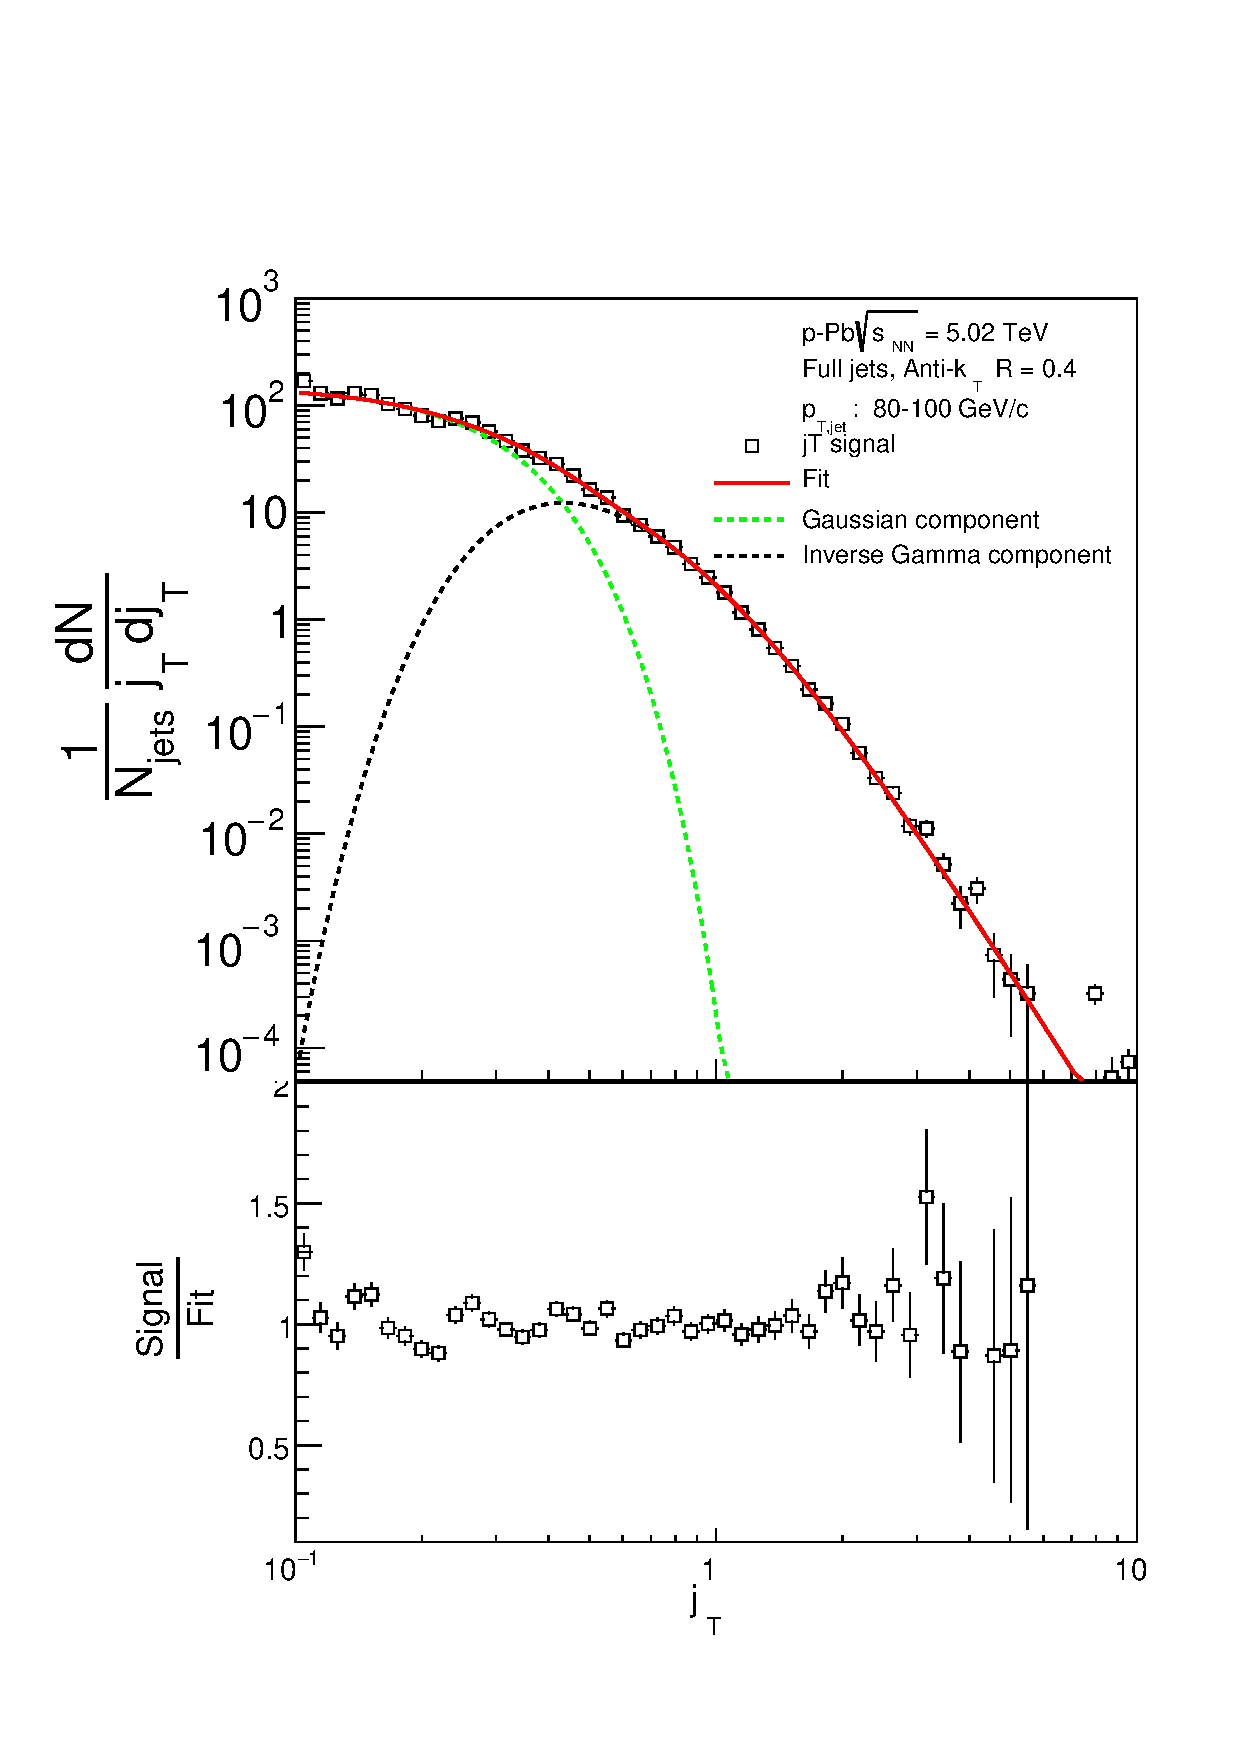
\includegraphics[width=0.95\textwidth]{results/JetConejTSignalFit/JetConejTSignalFitNFin00JetPt06randomBgBayes}
\end{subfigure}
\begin{subfigure}{0.24\textwidth}
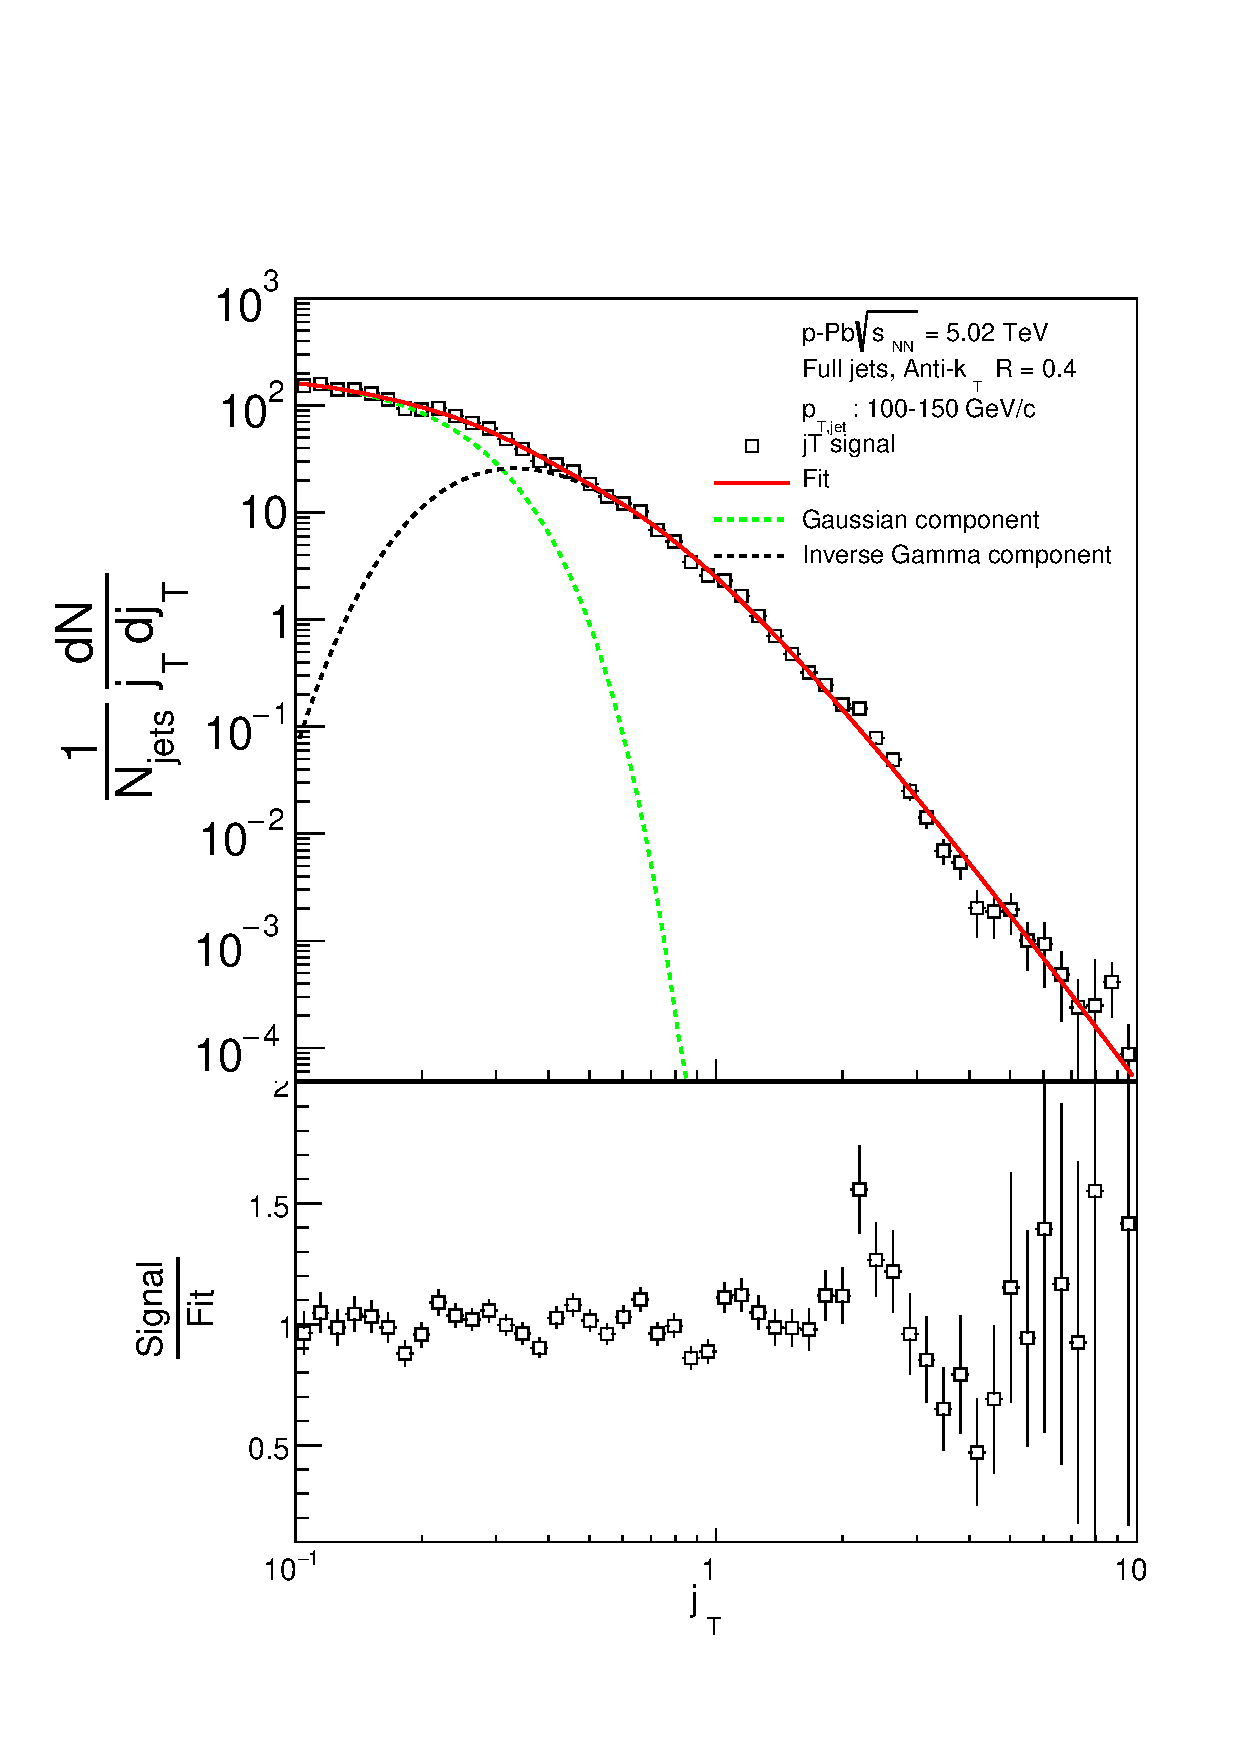
\includegraphics[width=0.95\textwidth]{results/JetConejTSignalFit/JetConejTSignalFitNFin00JetPt07randomBgBayes}
\end{subfigure}
\caption{$\jt{}$ signal with random bacgkround subtraction fits in different jet $\pt{}$ bins}
\label{fig:fitsrandombg}
\end{figure}

\begin{figure}
\centering
\begin{subfigure}{0.24\textwidth}
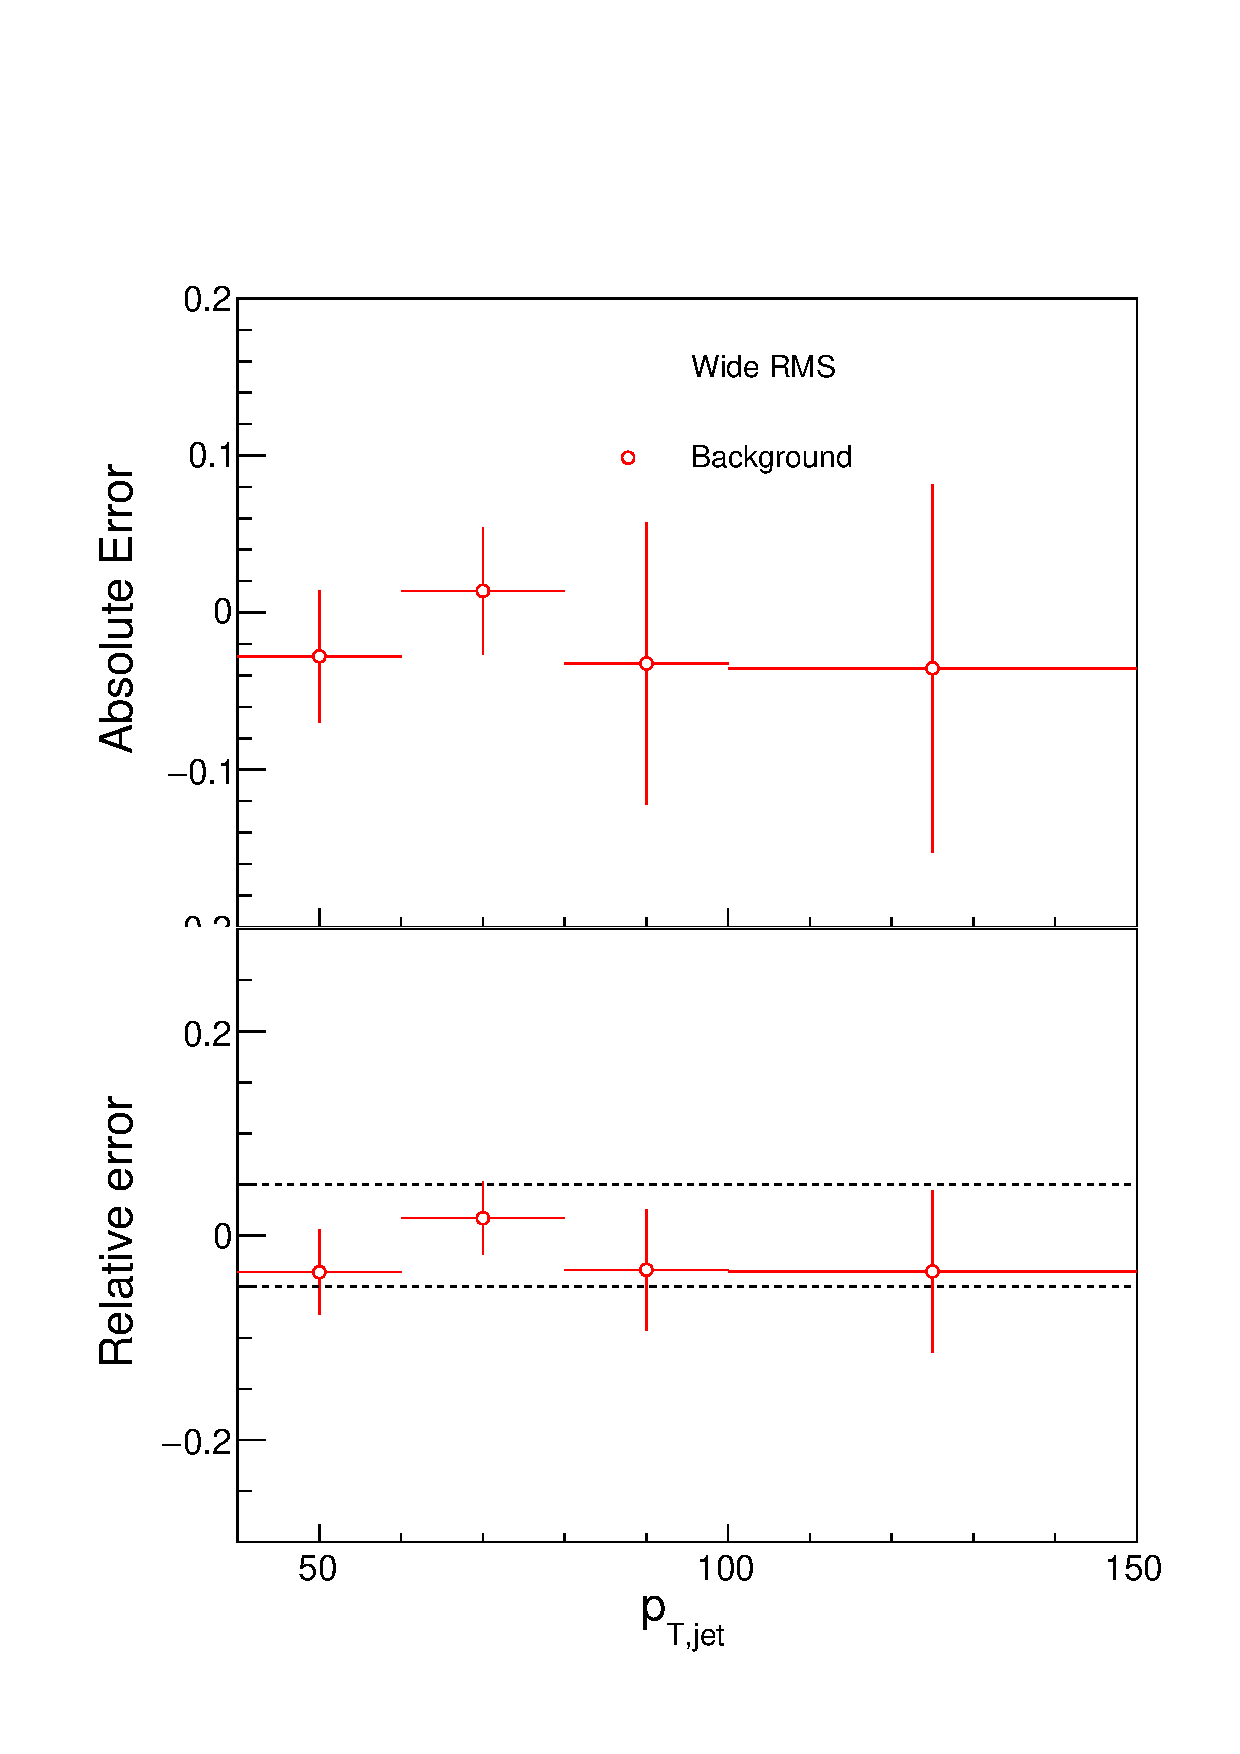
\includegraphics[width=0.95\textwidth]{results/SystematicErrors/SystematicErrorsGammaRMS_BgNFin00JetPt08_linx_data}
\end{subfigure}
\begin{subfigure}{0.24\textwidth}
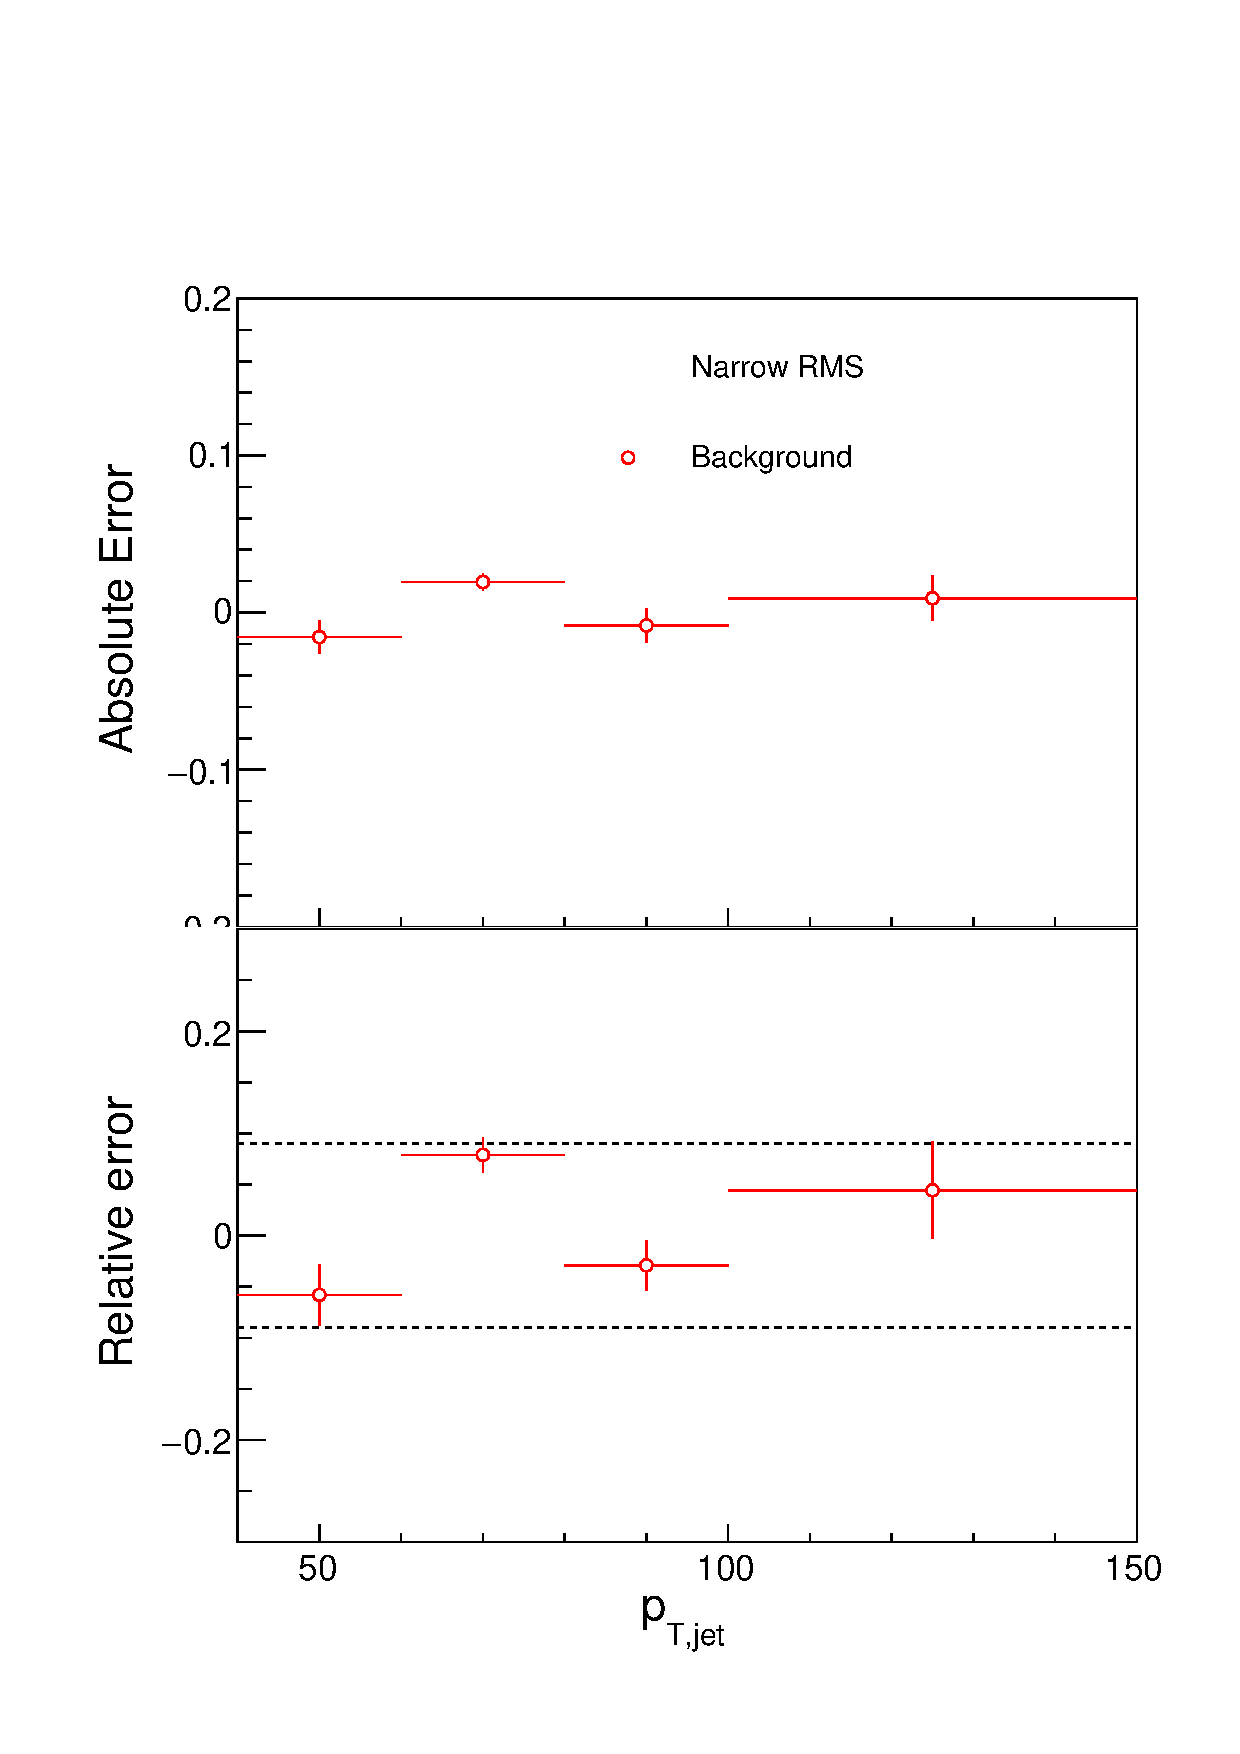
\includegraphics[width=0.95\textwidth]{results/SystematicErrors/SystematicErrorsGausRMS_BgNFin00JetPt08_linx_data}
\end{subfigure}
\caption{Differences between perpendicular cone and random background subtraction in the resulting RMS values.}
\label{fig:systbg}
\end{figure}

  
  
  
  \subsection{Unfolding}
Unfolding is the second major source of systematic uncertainty. To estimate the uncertainty related to the unfolding procedure several checks are performed. The main systematic uncertainty estimation comes from comparing results performed using both SVD and Bayesian unfolding. Difference between the methods is taken as the systematic error. Since SVD unfolding does not have a 2 dimensional options, the unfolding is done bin by bin. The resulting distributions after SVD unfolding and background subtraction with the perpendicular cone method are shown in fig \ref{fig:fitsSVD}. 

As in the background systematic estimation, fits are performed for both cases separately. Resulting differences between the methods for different components are shown in figure \ref{fig:systunf}. The dotted lines are at $\pm \unit[8]{\%}$ for both components. These are taken to be the systematic uncertainty related to unfolding. 

\begin{figure}
\centering
\caption{Resulting signal distributions from SVD unfolding with the perpendicular cone background methods. These are compared to the results from the Bayesian algorithm to estimate the systematic uncertainty.}
\label{fig:fitsSVD}
\end{figure}
\begin{figure}
\centering
\begin{subfigure}{0.24\textwidth}
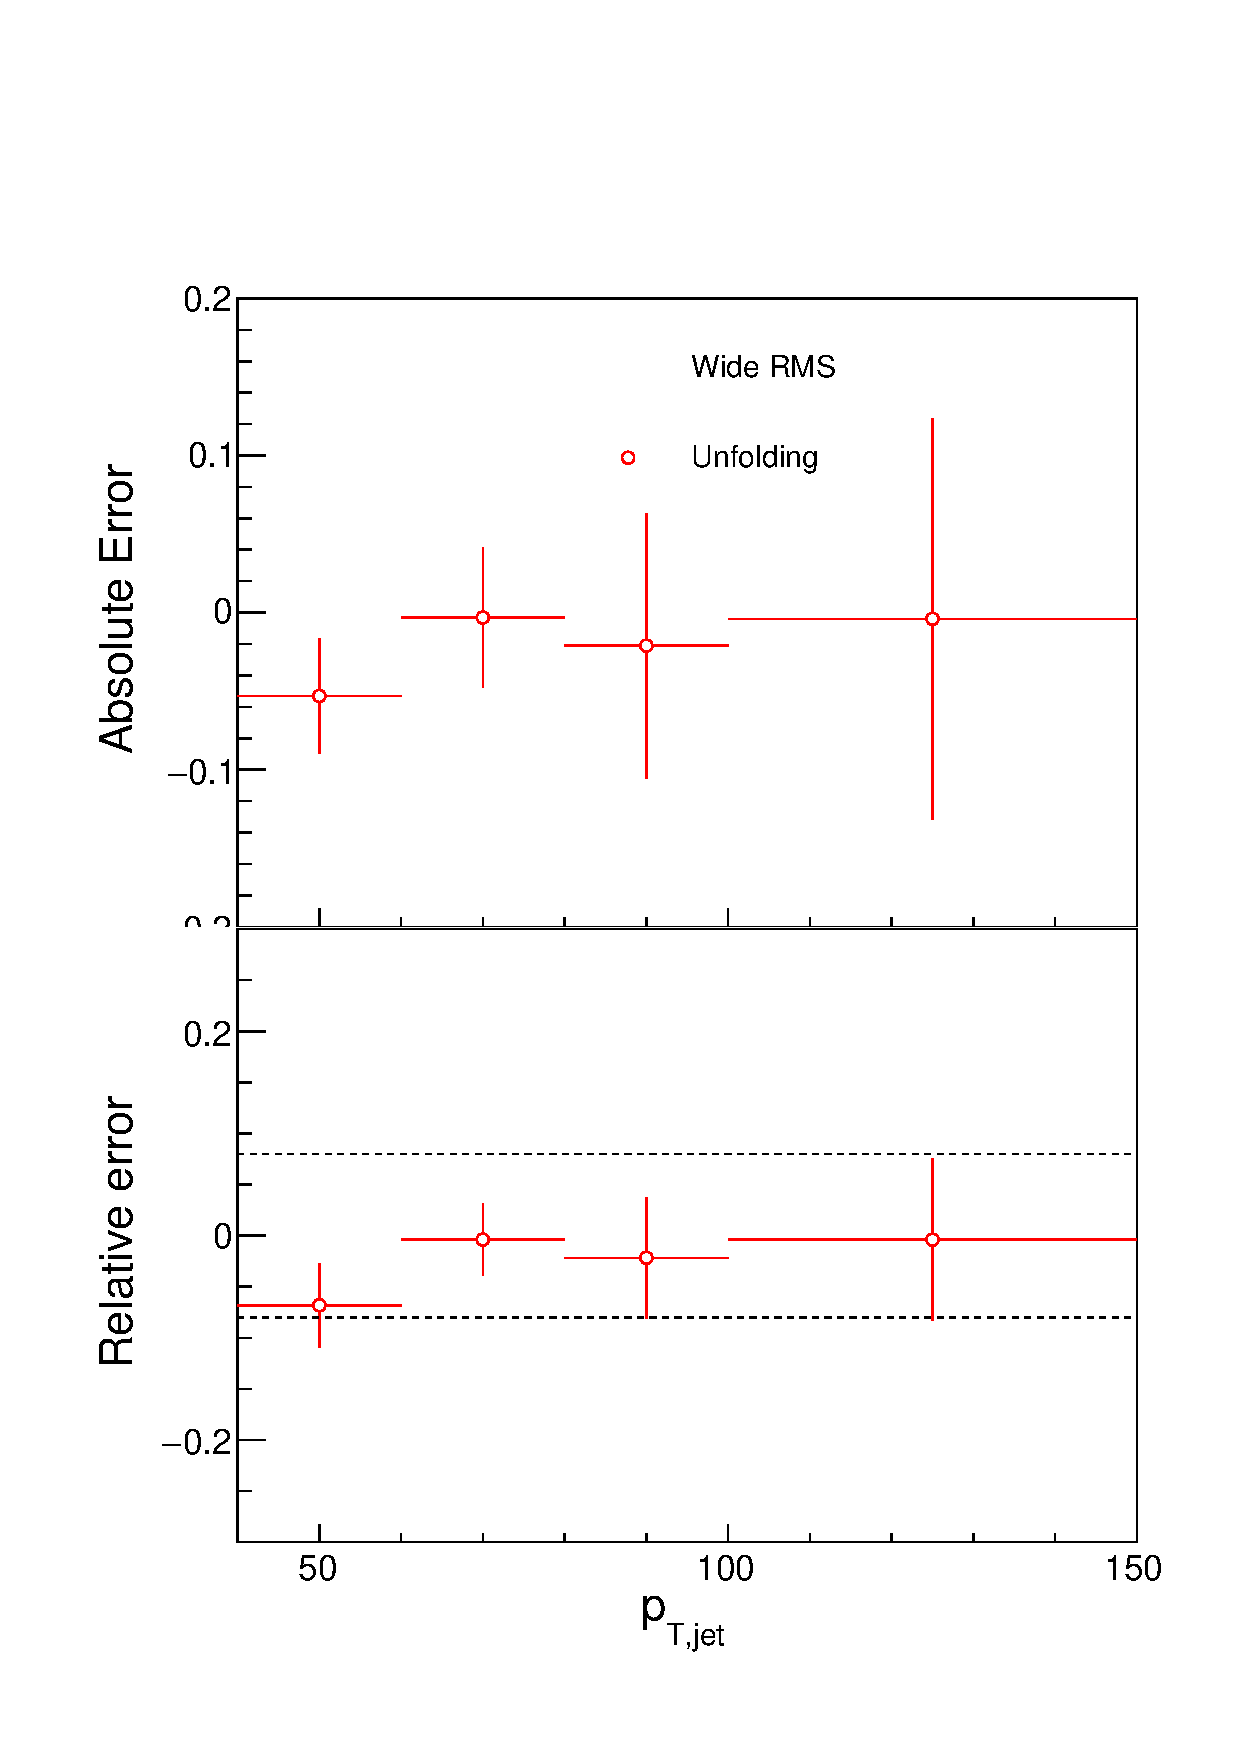
\includegraphics[width=0.95\textwidth]{results/SystematicErrors/SystematicErrorsGammaRMS_UnfNFin00JetPt08_linx_data}
\end{subfigure}
\begin{subfigure}{0.24\textwidth}
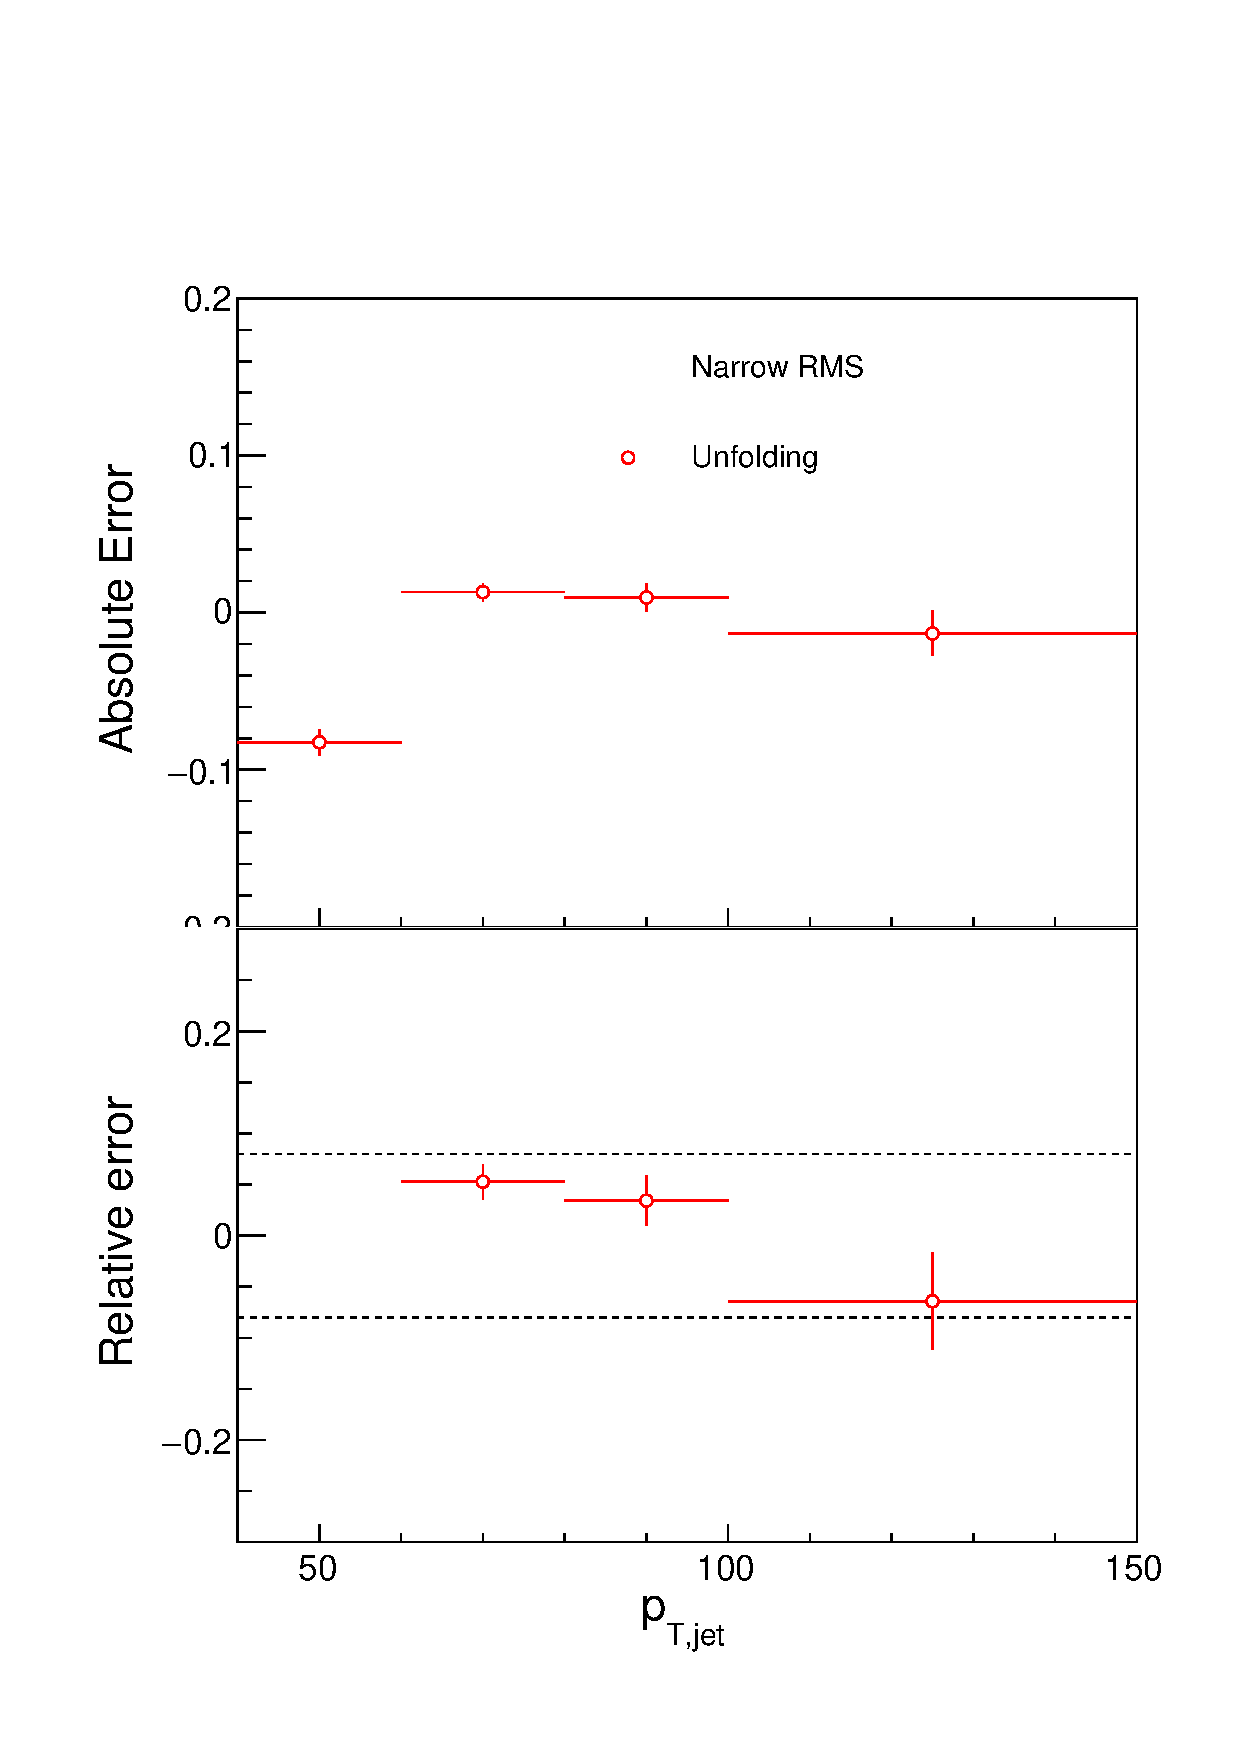
\includegraphics[width=0.95\textwidth]{results/SystematicErrors/SystematicErrorsGausRMS_UnfNFin00JetPt08_linx_data}
\end{subfigure}
\caption{Differences between Bayesian and SVD unfolding in the resulting RMS values}
\label{fig:systunf}
\end{figure}

Several other systematic checks were performed with the Bayesian unfolding procedure. They are described in the following sections. As these are small compared to the main uncertainty they are not included separately.
 
  
\subsubsection{Effect of number of iterations}
\label{sec:iterations}
The iterative unfolding algorithm permits the change of number of iterations. The unfolding procedure was carried out using different numbers of iterations. The results from these different cases are shown in Fig.~\ref{fig:iterations}. The results are compared to the default unfolding algorithm with 4 iterations. The difference in results between the different cases is mostly less than 2.5\%.
\begin{figure}
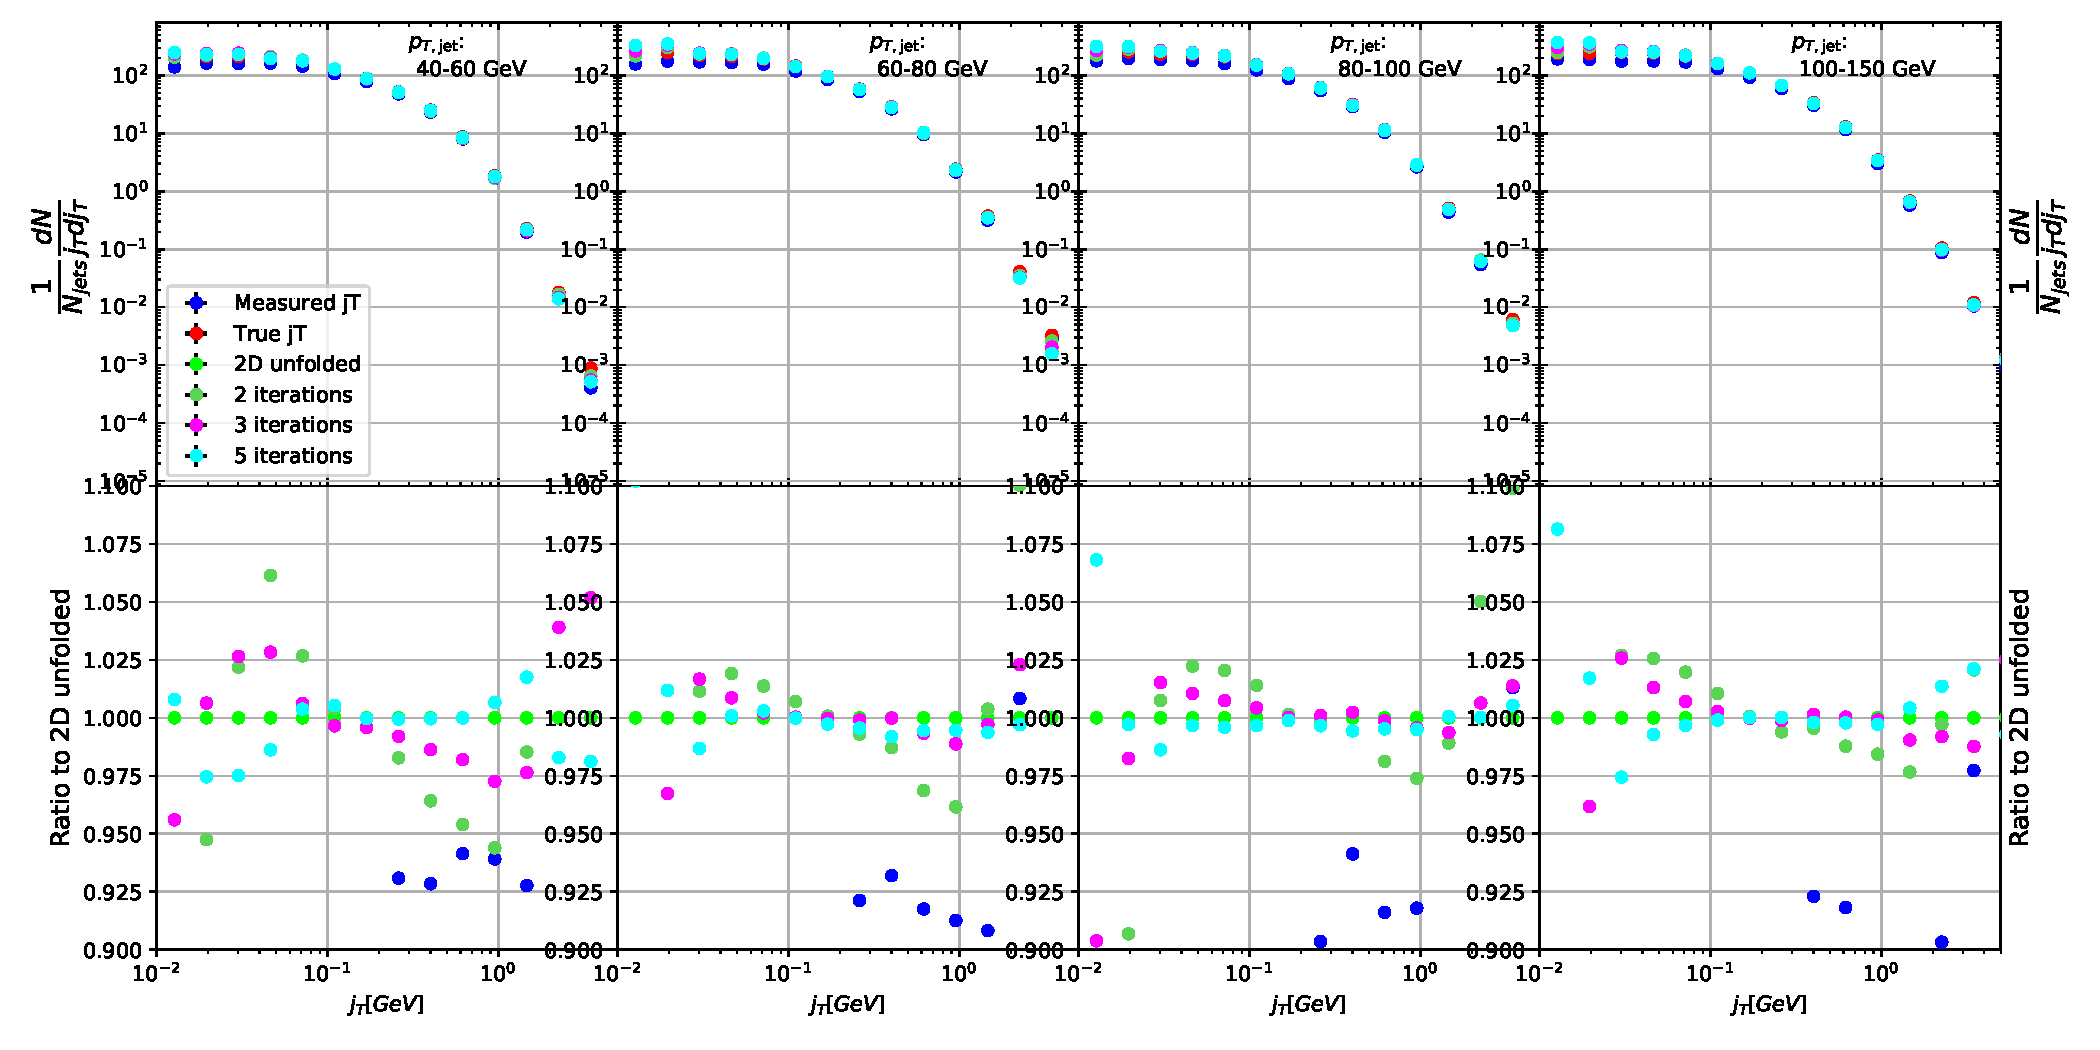
\includegraphics[width=0.99\textwidth]{figures/systematics/IterationsComparison.pdf}
\caption{Unfolding with different number of iterations}
\label{fig:iterations}
\end{figure}

\subsubsection{Effect of different prior}
\label{sec:prior}
The iterative algorithm requires a prior estimate of the shape of the distribution. As a default prior the truth (particle level) distribution is used. To test the effect of changing the prior we instead use the unfolded $\jt{}$ distribution as prior. The results are compared to the unfolding algorithm with the default prior. This is shown in Fig.~\ref{fig:prior} The difference in results between the different cases is mostly less than 2.5\%. 

\begin{figure}
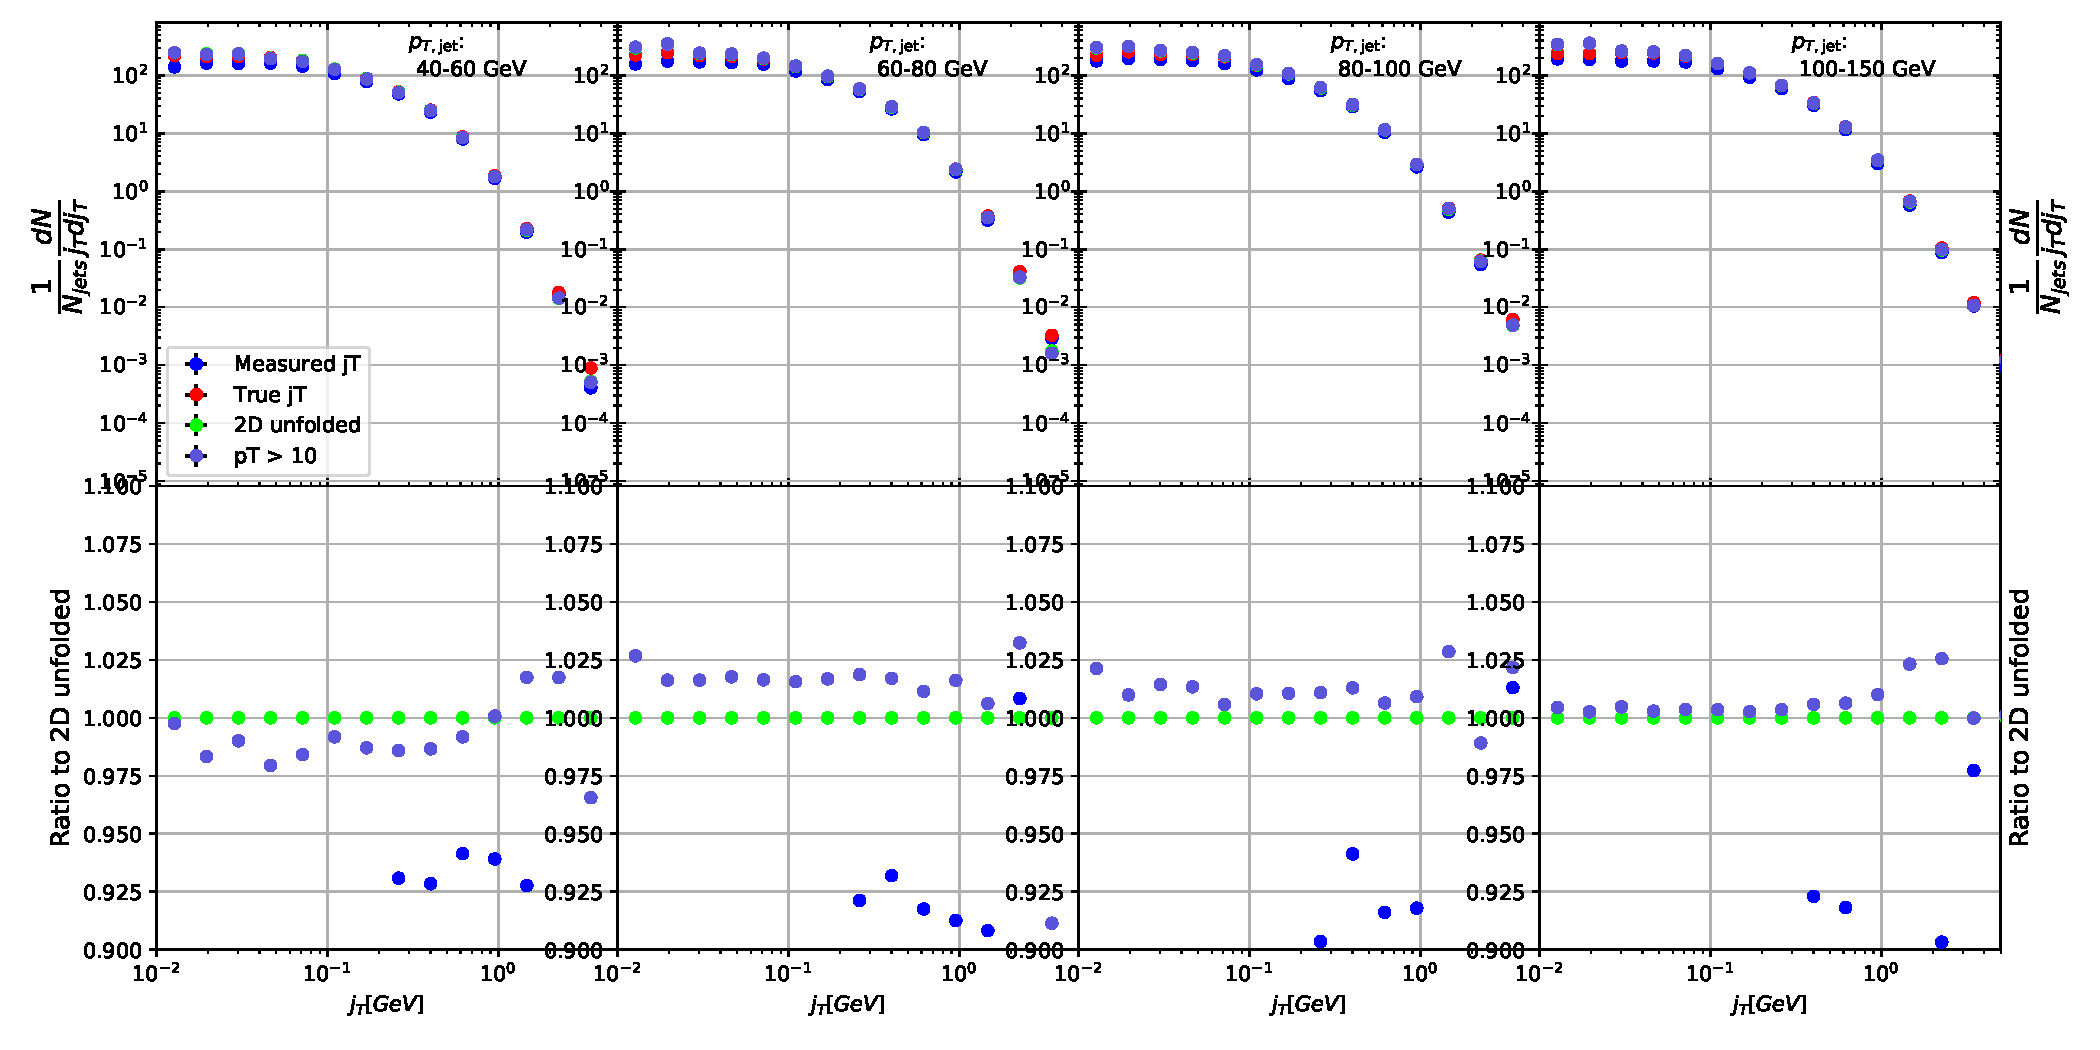
\includegraphics[width=0.99\textwidth]{figures/systematics/PtCutComparison10.pdf}
\caption{Effect of changing minimum jet $\pt{}$ used in unfolding from 5 to 10 \gev. {\color{red} Wrong figure}}
\label{fig:prior}
\end{figure}

\subsubsection{Effect of $\pt{}$ truncation}
\label{sec:truncation}
As an additional check the unfolding is carried out with different $\pt{jet}$ truncation values. By default the full range of $\pt{jet} > 5 \gev$ is used. We test the unfolding by only using the response matrix for $\pt{jet} > \unit[10]{\gev}$. The results of this test are shown in Fig.~\ref{fig:truncation}. The effects are strongest in the lower $\pt{jet}$ bins. Also in this case the difference is less than \unit[2.5]{\%} in all $\pt{jet}$ bins.

\begin{figure}
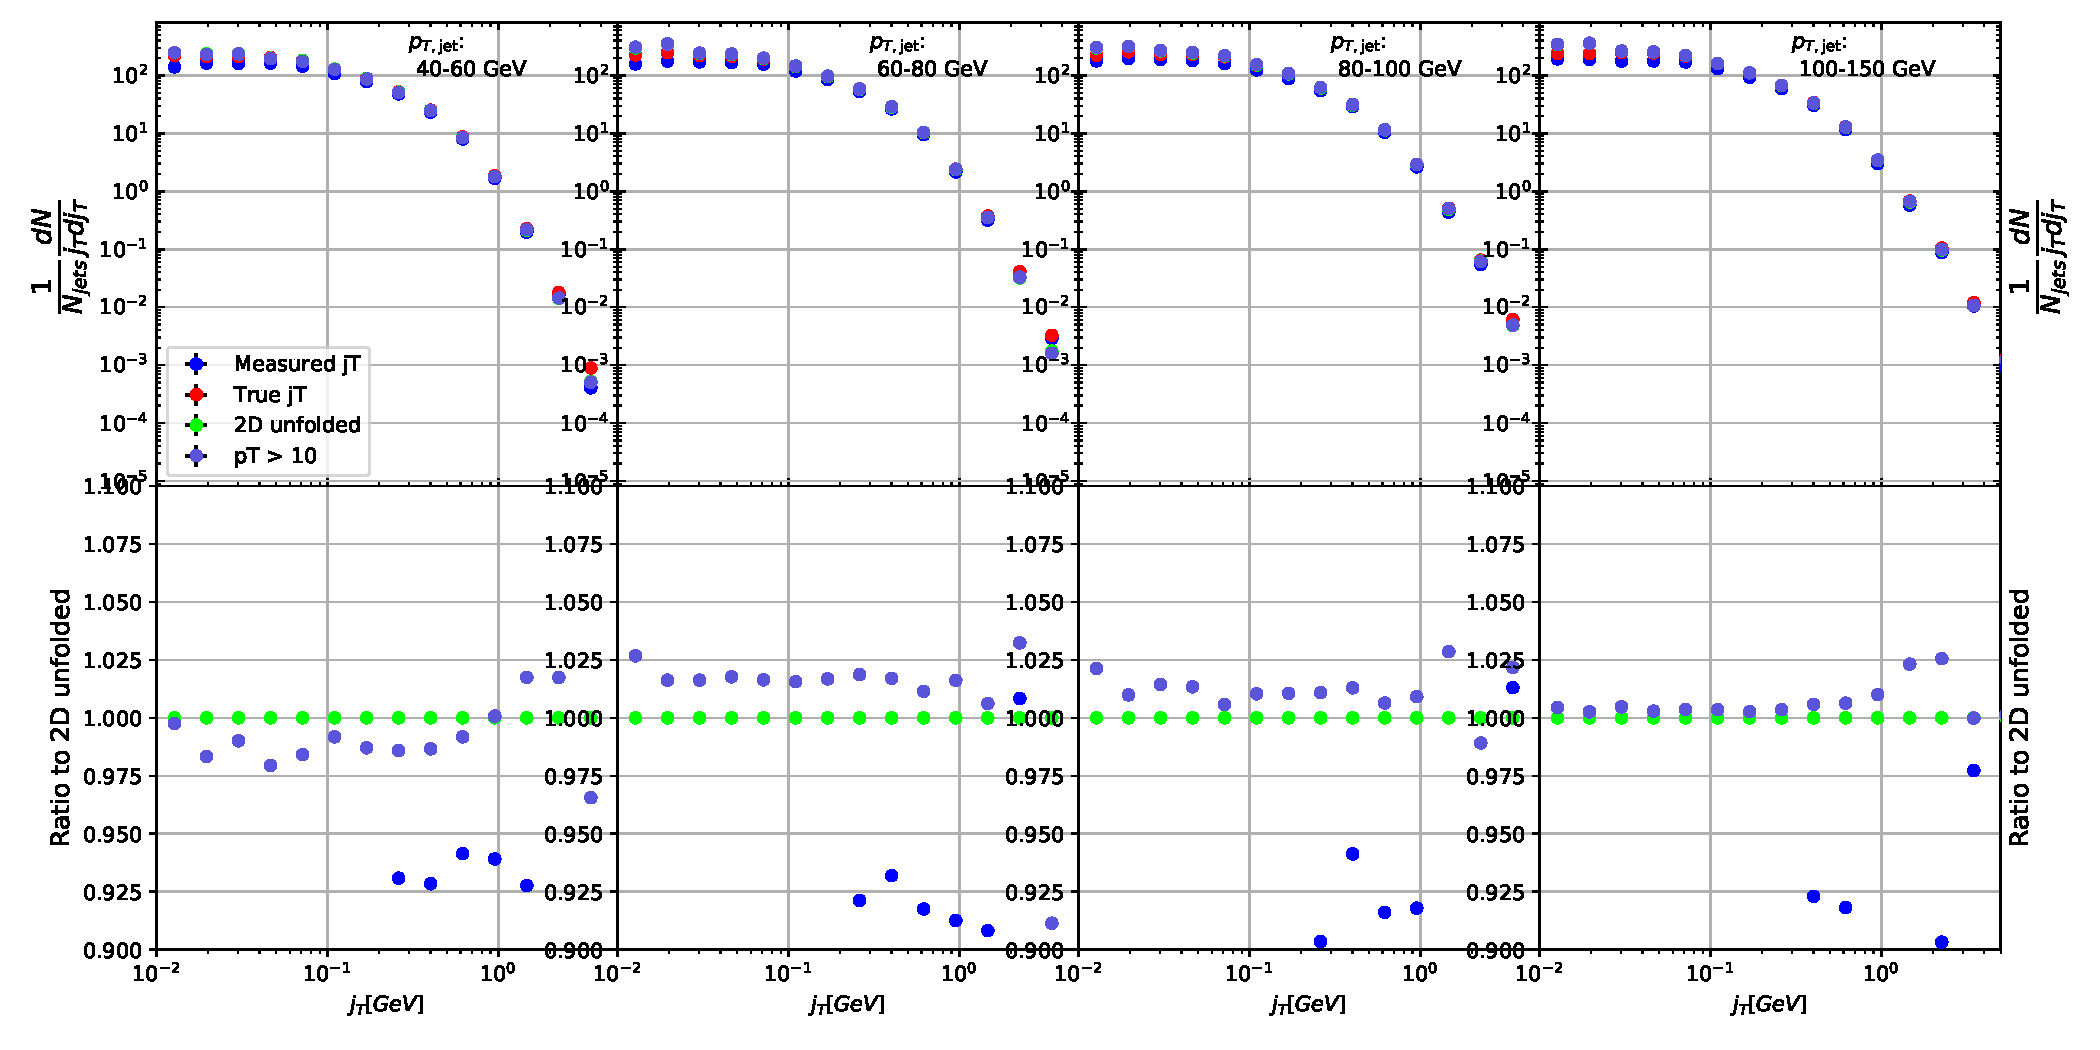
\includegraphics[width=0.99\textwidth]{figures/systematics/PtCutComparison10.pdf}
\caption{Effect of changing minimum jet $\pt{}$ used in unfolding from 5 to 10 \gev}
\label{fig:truncation}
\end{figure}

\subsection{Tracking}
Systematic effects originating from uncertainty in the tracking efficiency are estimated through a \pythia~simulation, where an artificial inefficiency of 3\% is introduced i.e. 3 \% of tracks are randomly removed from each event. The effect of this artificial inefficiency is shown in Fig.~\ref{fig:trackingsyst}. The systematic uncertainties assigned to tracking efficiency are \unit[4]{\%} for the narrow component and \unit[5]{\%} for the wide component. 

\begin{figure}
\centering
\begin{subfigure}{0.45\textwidth}
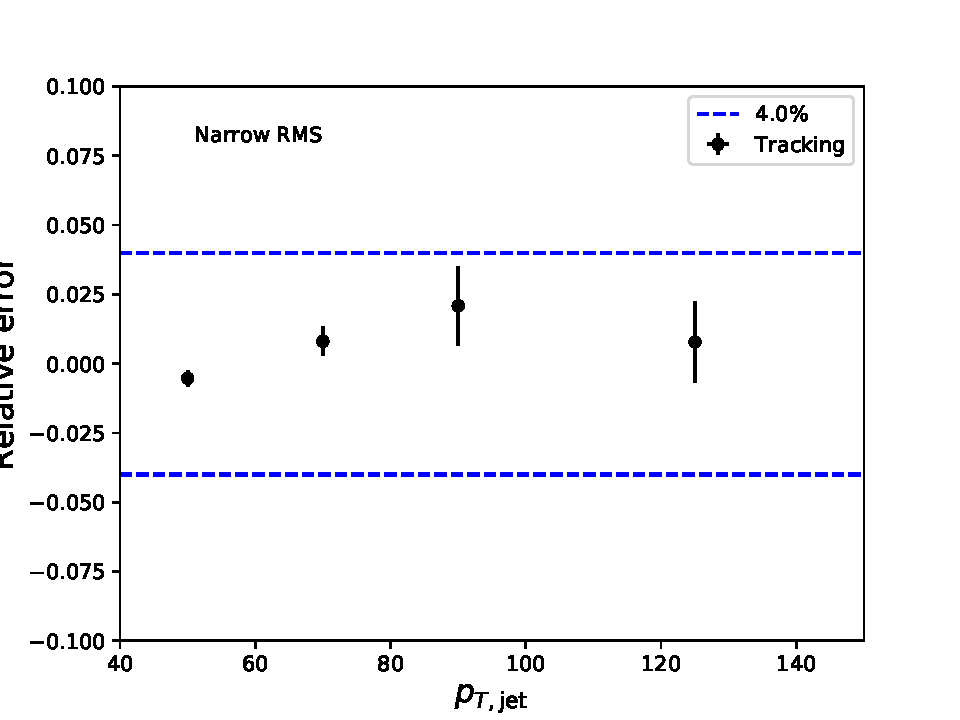
\includegraphics[width=0.95\textwidth]{figures/systematics/SystematicErrorsGausRMS_Tracking.pdf}
\end{subfigure}
\begin{subfigure}{0.45\textwidth}
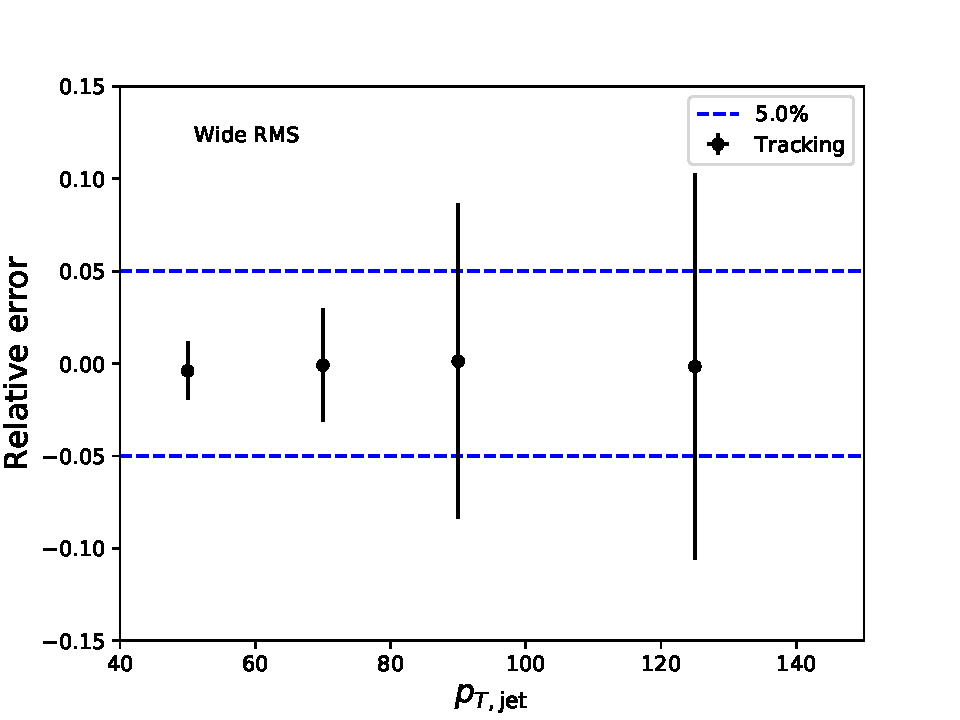
\includegraphics[width=0.95\textwidth]{figures/systematics/SystematicErrorsGammaRMS_Tracking.pdf}
\end{subfigure}
\caption{Relative systematic errors resulting from tracking efficiency uncertainty.}
\label{fig:systtrack2}
\end{figure}

\subsection{EMCal clusters}
The analysis uses EMCal clusters only in the reconstruction of jets. Thus the only way uncertainty in EMCal performance can affect the results is through modification of jet momentum or axis.
  
Uncertainty related to the EMCal energy scale was estimated by scaling cluster energies up and down by 2 \% in a PYTHIA particle level simulation. Similarly the jet momentum was scaled by $\pm 2\%$ when determining the jet $\pt{}$ bin. In the analysis EMCal is used only in jet reconstruction, not for calculating $\jt{}$. The only ways EMCal uncertainty can affect the analysis are changes in jet energy and jet axis. Jet axis shouldn't significantly change, so the main contribution should be changes in jet $\pt{}$ bin.

The resulting differences in the inclusive $\jt{}$ distributions are shown in Fig.~\ref{fig:systemcal}. Qualitatively the effect of scaling cluster energies is the same as scaling the jet energies.

Like in the previous cases fits are performed for the unscaled case and for cases with $\pm \unit[2]{\%}$ scaling. The resulting systematic uncertainties are shown in Fig.~\ref{fig:systemcal2}. The uncertainty is taken to be 1\% for both components.

\begin{figure}
\centering
\begin{subfigure}{0.90\textwidth}
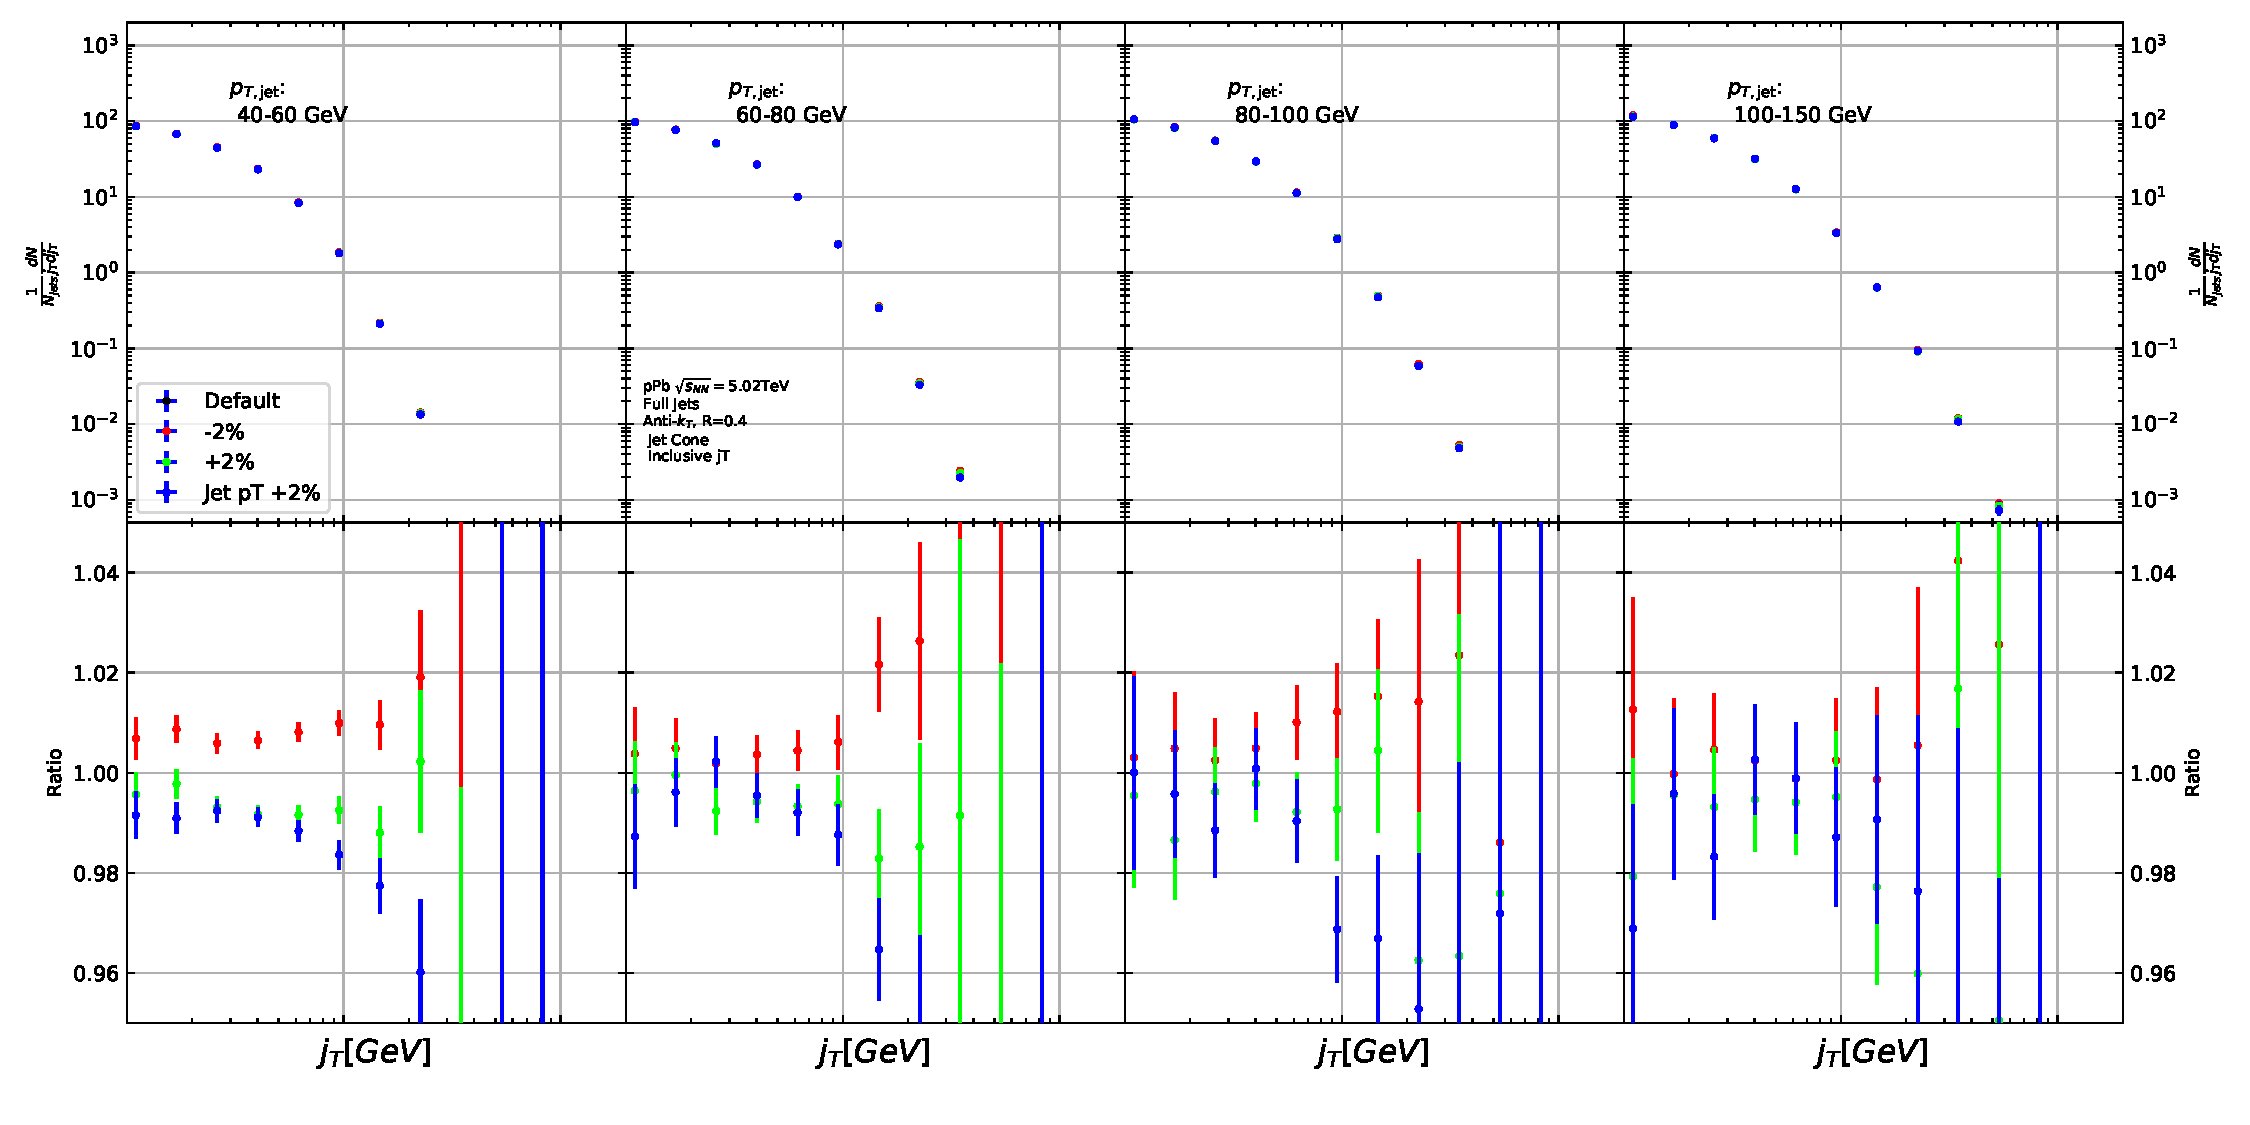
\includegraphics[width=0.95\textwidth]{figures/systematics/HadCorrComparisonJetPt4To8.pdf}
\end{subfigure}
%\begin{subfigure}{0.24\textwidth}
%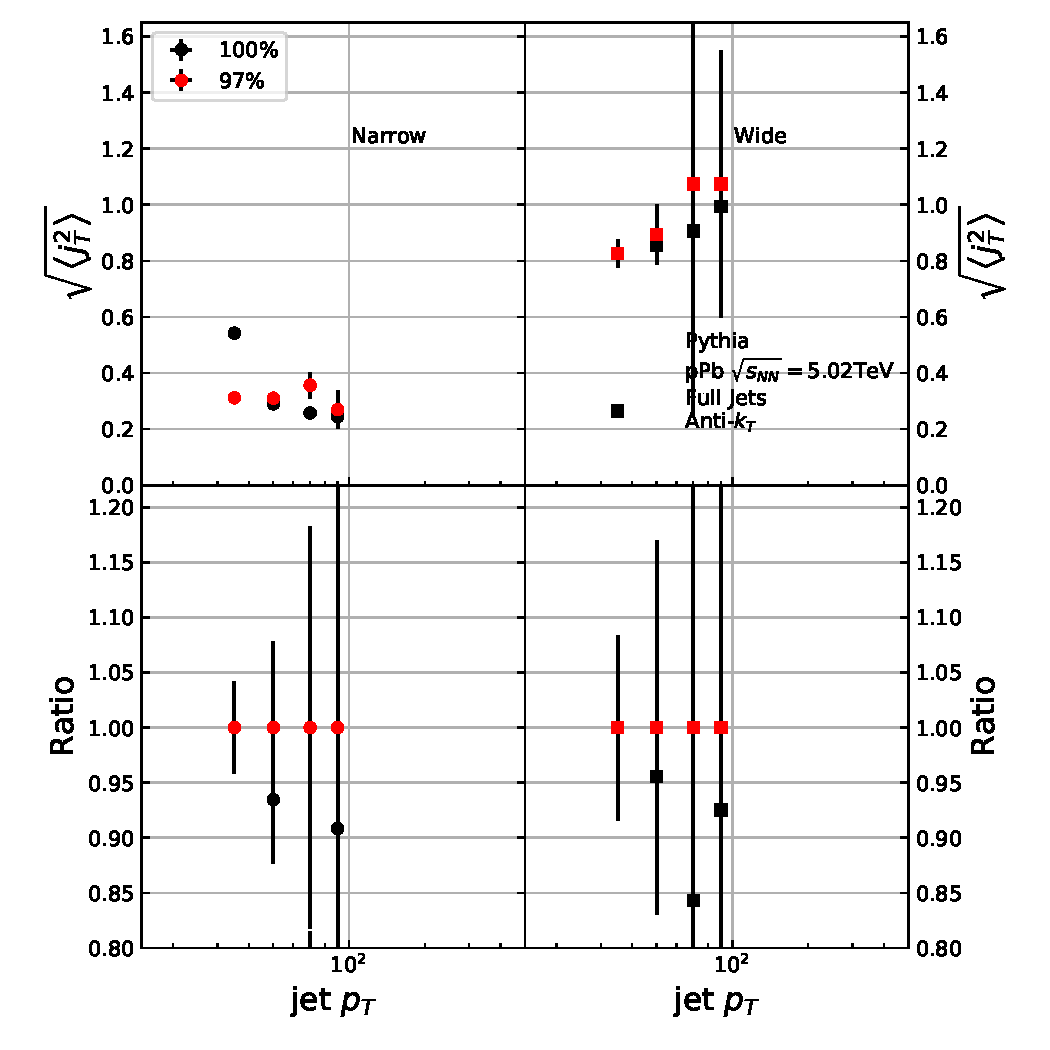
\includegraphics[width=0.95\textwidth]{RooUnfold/PythonFigures/TrackingSystematicsRMS.pdf}
%\end{subfigure}
\caption{Results from PYTHIA simulations with Cluster energies scale up/down by 2 \%. Additionally jet momenta were scaled by 2 \% when determining the jet $\pt{}$ bin.}
\label{fig:systemcal}
\end{figure}

\begin{figure}
\centering
\begin{subfigure}{0.45\textwidth}
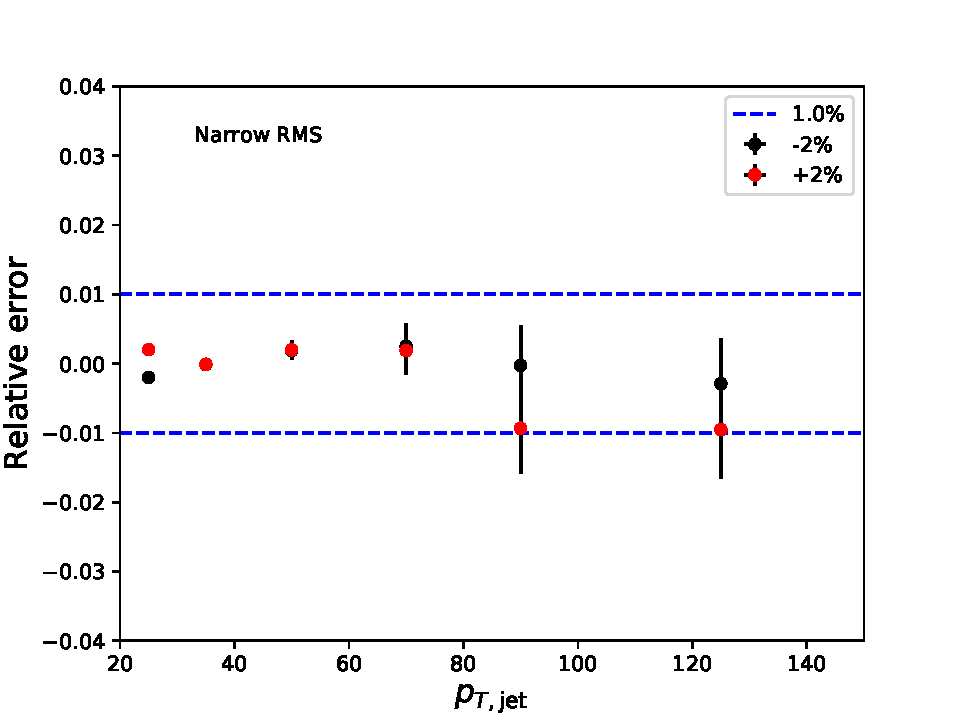
\includegraphics[width=0.95\textwidth]{figures/systematics/SystematicErrorsGausRMS_Emcal.pdf}
\end{subfigure}
\begin{subfigure}{0.45\textwidth}
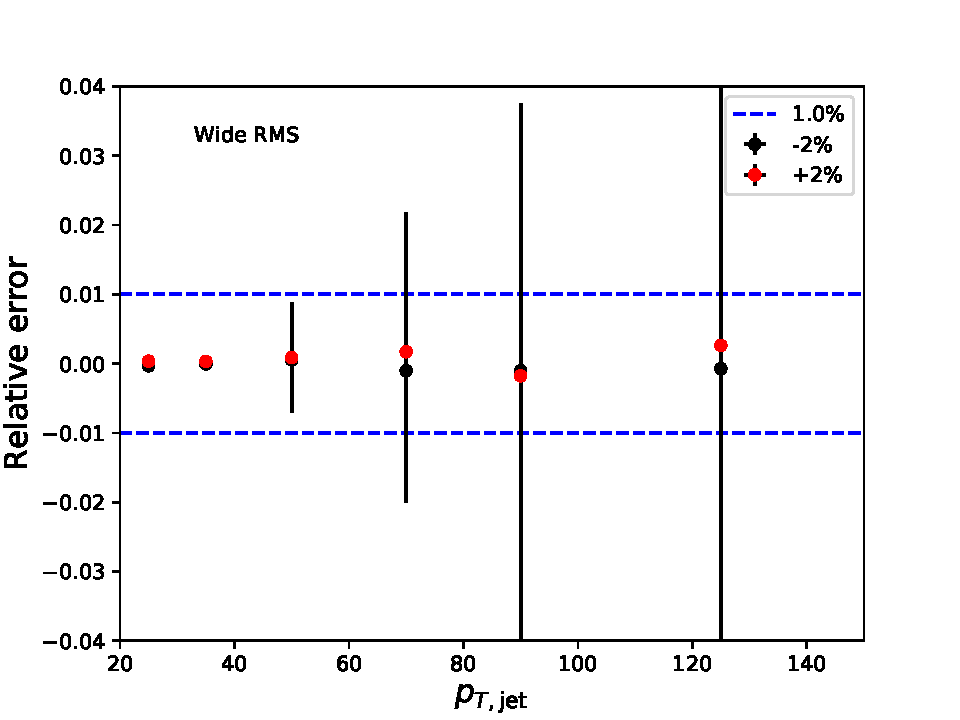
\includegraphics[width=0.95\textwidth]{figures/systematics/SystematicErrorsGammaRMS_Emcal.pdf}
\end{subfigure}
\caption{Relative systematic errors resulting from cluster energy uncertainty.}
\label{fig:systemcal2}
\end{figure}



\subsection{Summary/Combining systematics}
The different source of the systematic uncertainty are considered as uncorrelated and the values of each source are summed in quadrature.

Resulting systematic errors are shown in table \ref{tab:systematics}. The different source of the systematic uncertainty are considered to be uncorrelated and are thus combined bin-by-bin in quadrature to get the total systematic errors.  The resulting uncertainty is approximately 9 \% for the wide component RMS and 12 \% for the narrow component RMS. 
\begin{table}[htb]
\centering
\caption{Summary of systematic errors}
\label{tab:systematics}
\begin{tabular}{ l | c | r }
  Systematic & Wide RMS & Narrow RMS \\
    \hline			
  Background & 5 \% & 9 \% \\
  Unfolding & 8 \% & 8 \% \\
  Tracking & 4 \% & 5 \% \\ 
  EMCal & 1 \% & 1 \% \\
  Total & 10 \% & 13\% \\
  \hline
  \end{tabular}
  \end{table}

  
\subsection{Additional checks}
\subsubsection{Comparison between A and C side}
In 2013 there were issues with tracking. To rule out effects on $\jt{}$ distributions a study was performed comparing $\jt{}$ distributions between A and C side. {\color{red}Which is lead going side and which is proton going} No systematic differences were observed. Figure~\ref{fig:signalbg} shows the comparison between inclusive distributions between the different sides, both for minimum bias and EMCal triggered datasets.

\begin{figure}
\centering
\begin{subfigure}{0.95\textwidth}
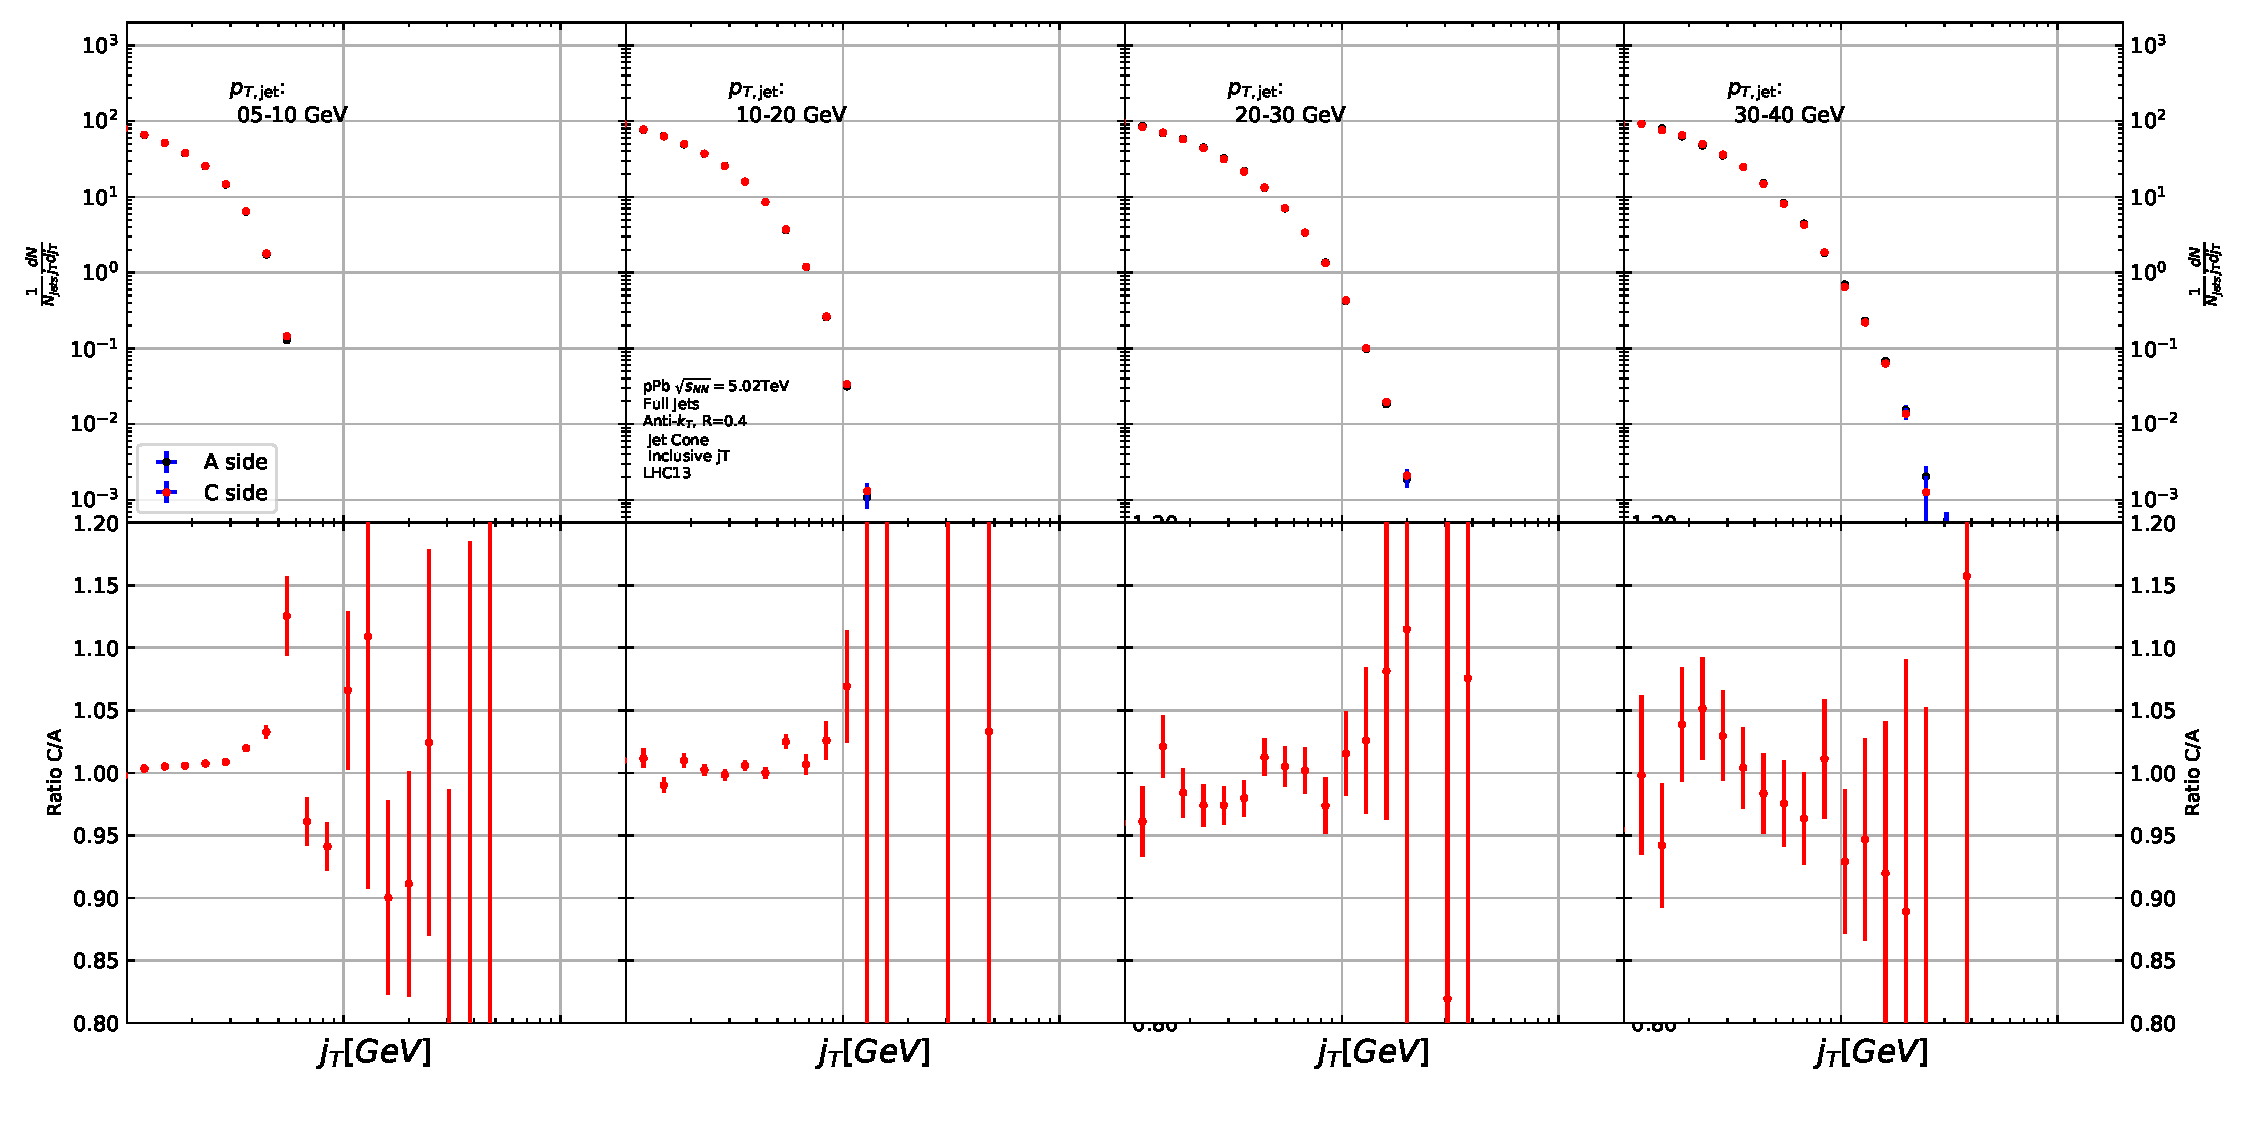
\includegraphics[width=\textwidth]{pics/ACsideComparison/ACsideJetConeJtInclusivePtFrom0To4LHC13.pdf}
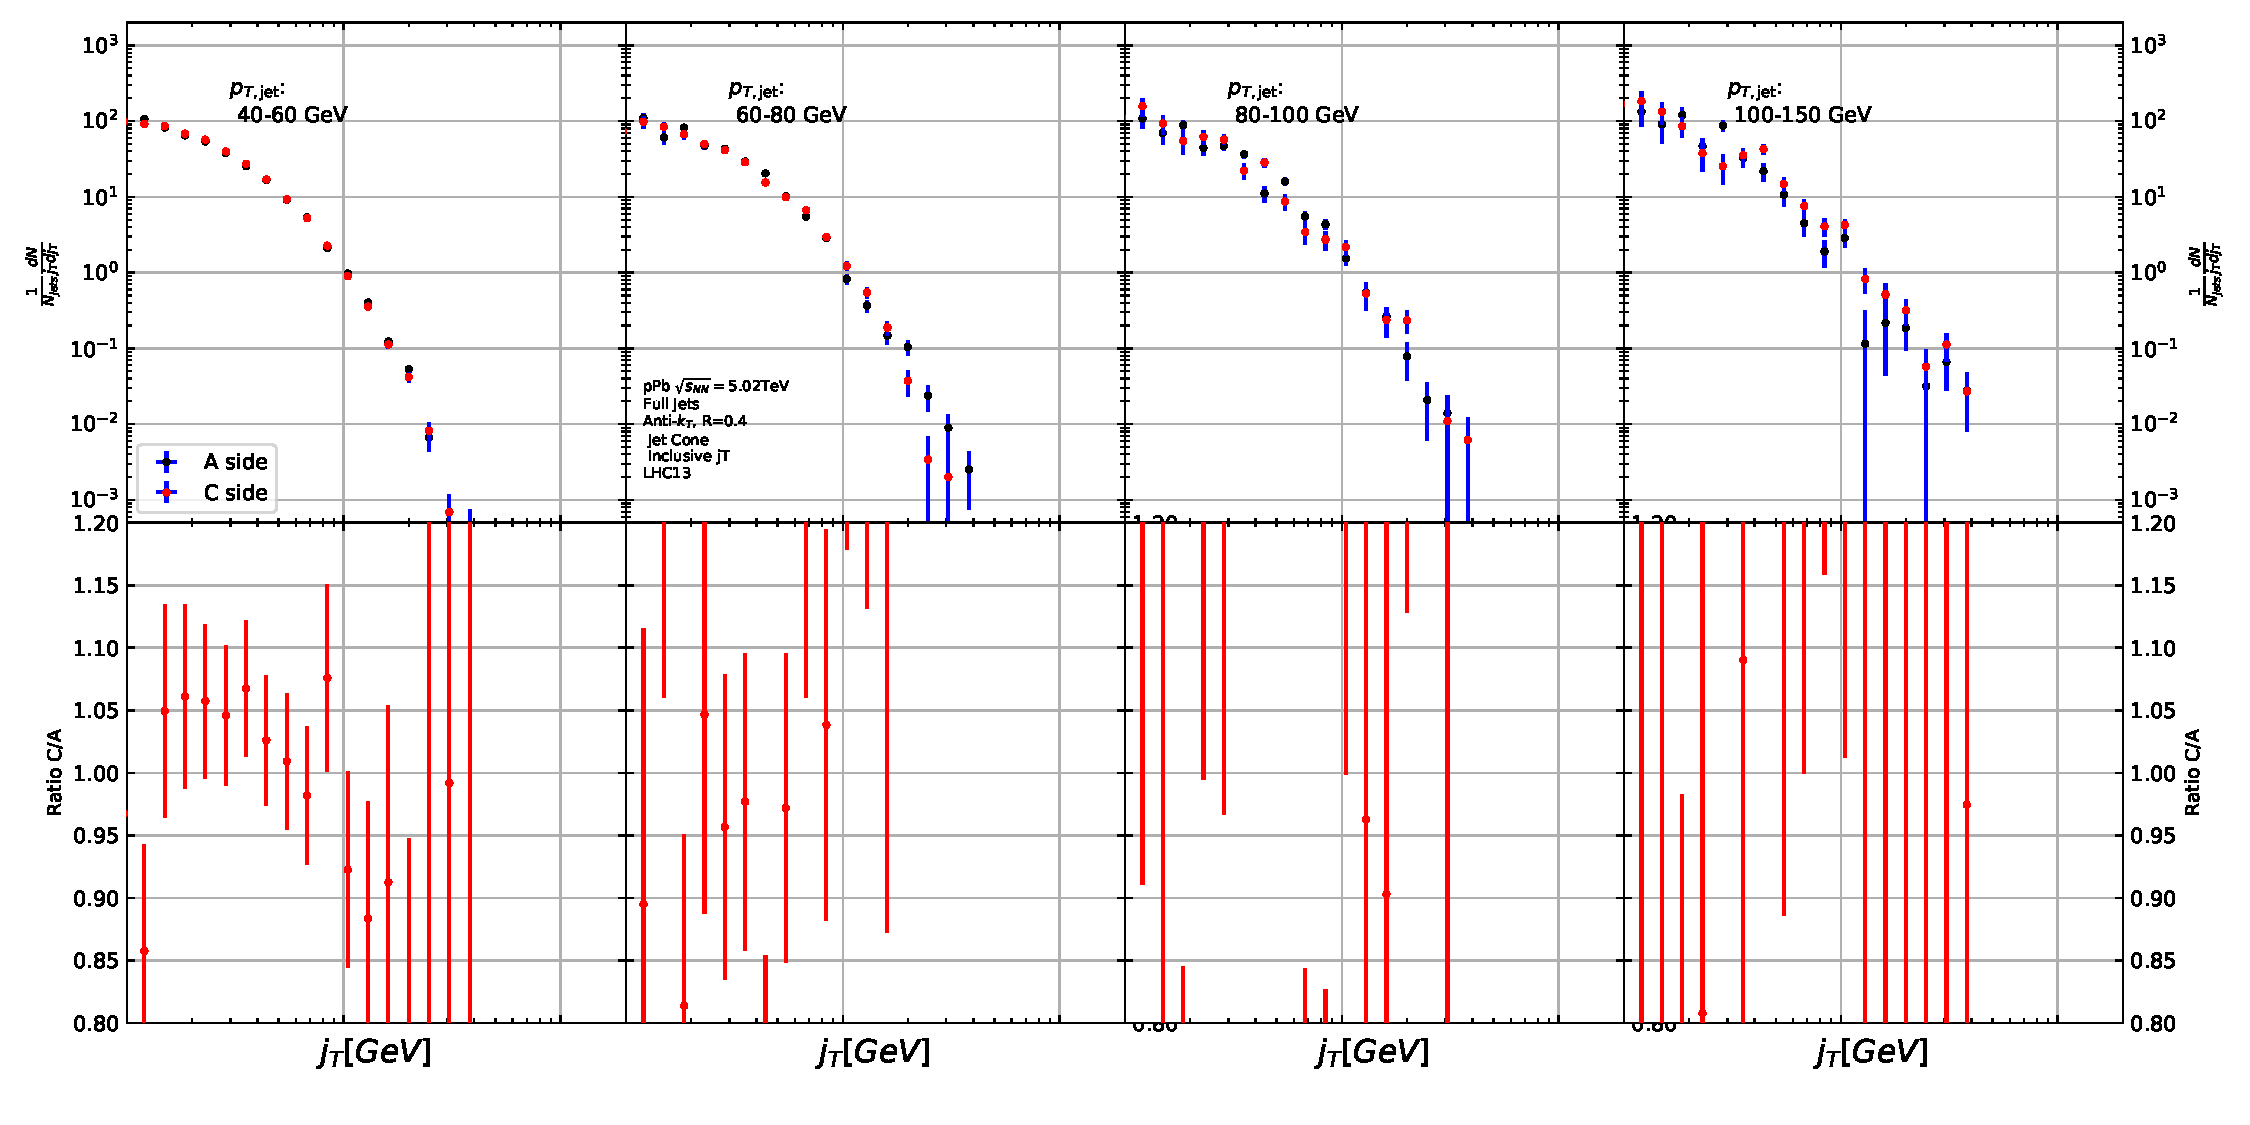
\includegraphics[width=\textwidth]{pics/ACsideComparison/ACsideJetConeJtInclusivePtFrom4To8LHC13.pdf}
\includegraphics[width=\textwidth]{pics/ACsideComparison/ACsideJetConeJtInclusivePtFrom4To8LHC13EMCal.pdf}
%Tag 20170810 python2.7 Python/DrawSignal.py legotrain_CF_pPb-1053_20170223-2002_LHC13bcde.root
\end{subfigure}
\caption{Comparison of inclusive $\jt{}$ distributions between A and C side for minimum bias and EMCal triggered data.}
\label{fig:signalbg}
\end{figure}


%% !TEX root = thesis.tex

\section{Flow fluctuations and unfolding}
The flow coefficients are not constant event-by-event, because of the fluctuations. The $v_n$ distributions are important observables in heavy-ion collisions. However the experimental methods have their own uncertainties and they smear the distribution. To get the true distribution one must be able to remove these effects.

The process of removing the smearing from experimental methods is known as unfolding. Unfolding can be used to get the true distribution from the observed distribution. In this thesis I am using a Bayesian unfolding method from~\cite{dagostini1995} which I first apply to a Toy Monte Carlo simulation and afterwards to AMPT data.

\FloatBarrier
\subsection{Unfolding in AMPT}
I applied the same unfolding method to AMPT. I calculated $\bar v_n^{obs}=\left(v_{n,x}^{obs},v_{n,y}^{obs}\right)$ for particles in mid-rapidity $|\eta|<0.8$ and $p_T>0.1\gevc$. Statistics used for each centrality bin as well as average $v_n$ coefficients are shown in Table \ref{tab:amptunfold}. The unfolding results for $v_2$ and $v_3$ are shown in Fig.~\ref{fig:AMPTunfoldvn}. For $v_2$ the average value for peripheral collisions is large enough to provide accurate unfolding based on the toy monte carlo simulation. Also for the central collisions the multiplicity is high enough even though the average $v_2$ is in the range with worse unfolding performance. The unfolded $v_2$ distributions should therefore match the true distribution well. 

\begin{table}[htbp]
\centering
\begin{tabular}{ l  | c | c | c | c | c | c}
\small Centrality 					&	0-5\%	&5-10\%	&10-20\%	&20-30\%	&30-40\%	&40-50\% \\
\hline
Events	& 56733	& 66579	 & 71023 & 84566	& 80033	& 415425 \\
$\left<N_{ch}\right>(|\eta|<0.8,$ & 2423  & $1971$ & 1471 & 990 & 647 & 401 \\
$\,p_T>0.1\gevc )$ & & & & & & \\

%Unfolding $ \left<v_2\right>$	&	0.0289641pm8,81685e-6		&0.040642 pm 9.6979e-06	& 0.0544602 pm 1.10077e-05	&0.071013 pm 1.16004e-05	&0.0849903 pm 1.29229e-05	& 0.0912794 pm 5.80083e-06 \\
Unfolding $ \left<v_2\right>$&	0.028 & 0.041 & 0.058 & 0.072 & 0.078 & 0.077\\
Unfolding $ \left<v_3\right>$ & 	0.016 & 0.018 & 0.018 & 0.016 & 0.012 & 0.0078\\
\hline
\end{tabular}
\caption{Number of events used in AMPT study and the average multiplicity used to calculate $v_2$ and $v_3$. Also shown are the average values of unfolded $v_2$ and $v_3$ distributions.}
\label{tab:amptunfold}
\end{table}

\begin{figure}[htp]
	\centering
        \begin{subfigure}[b]{0.95\textwidth}
                \centering
          	\includegraphics[width=\textwidth]{pics/AMPTunfoldedv2cents}
		\caption{Unfolded $v_2$ in AMPT}
	        	\label{fig:AMPTunfoldv2}
           \end{subfigure}
        \begin{subfigure}[b]{0.95\textwidth}
                \centering
          	\includegraphics[width=\textwidth]{pics/AMPTunfoldedv3cents}
		\caption{Unfolded $v_3$ in AMPT}
			        	\label{fig:AMPTunfoldv3}
           \end{subfigure}
           \caption{Unfolding results in AMPT}
             \label{fig:AMPTunfoldvn}
\end{figure}

It can be seen that the $v_2$ distributions in peripheral collisions do not look like the radial projection of a two dimensional gaussian shown in Eq.~(\ref{eq:gaussproj1}). This was the distribution used in the toy Monte Carlo and as an initial guess. 

The average value for $v_3$ stays at a relatively constant value of $~0.16$ between the different centrality bins until it drops at centralities larger than 40\%. In central collisions the multiplicity is however higher than the one used in the toy monte carlo. This might be enough for the method to provide accurate results. However in peripheral collisions the multiplicity is even below the values that were tested in the toy monte carlo simulation. At these values the unfolding method can not be expected to give accurate results.

The $v_n$ coefficients calculated with the unfolding are compared to corresponding values from the event plane method. This is shown in Fig.~\ref{fig:AMPTvnvsCent}. It can be seen that compared to the event plane method, unfolding gives higher values. In the toy monte carlo there was no difference between these methods.

For $v_3$ in peripheral collisions the distributions seem to agree. However this is expected in these events. In events with low multiplicity and low $v_3$ values the initial guess dominates the unfolding results and the initial guess is based on the event plane results. 

To get an estimate of the performance of unfolding in AMPT I ran the Toy Monte Carlo simulation using detected multiplicities and $ \left<v_n\right>$ values. The ratios of unfolded and input distributions are shown in Fig.~\ref{fig:AMPTcheck}. It can be seen that for $v_2$ the method seems to give accurate results, but for $v_3$ the agreement is only moderate in central collisions and fails completely in peripheral collisions.




\begin{figure}[htp]
	\centering
	\includegraphics[width=0.65\textwidth]{pics/AMPTvnvsCent}
	\caption{Unfolding and Event plane method $v_2$ in AMPT versus centrality. The error bars are too small to be seen in this figure.}
	\label{fig:AMPTvnvsCent}
	\end{figure}

%\begin{figure}[htpb]
%	\centering
%        \begin{subfigure}{0.49\textwidth}
%                \centering
%          	\includegraphics[width=\textwidth]{pics/AMPTv2unfolding}
%		\caption{$\left<v_2\right>=0.03$ }
%	        	\label{fig:amptunfoldv2}
%           \end{subfigure}
%           \hfill
%                   \begin{subfigure}{0.49\textwidth}
%                \centering
%          	\includegraphics[width=\textwidth]{pics/AMPTv2unfolding}
%		\caption{$\left<v_2\right>=0.02$ }
%	        	\label{fig:amptunfoldv3}
%           \end{subfigure}
%
%
%           
%           \caption{Unfolding results in AMPT for centrality 0-5\%}
%             \label{fig:amptunfold}
%\end{figure} 



\begin{figure}[htp]
	\centering
	        \begin{subfigure}[b]{0.49\textwidth}
	        \centering
	\includegraphics[width=\textwidth]{pics/v2inputRatios}
			\caption{$v_2$ }
	        	\label{fig:AMPTcheckv2}
           \end{subfigure}
           \hfill
           	        \begin{subfigure}[b]{0.49\textwidth}
	\includegraphics[width=\textwidth]{pics/v3inputRatios}
			\caption{$v_2$ }
	        	\label{fig:AMPTcheckv3}
           \end{subfigure}
           
	\caption{$v_n$ Unfolding results of the Toy Monte Carlo using parameters from AMPT study}
	\label{fig:AMPTcheck}
	\end{figure}

%% !TEX root = thesis.tex

\section{Correlations}
\subsection{Jet correlations}
\begin{itemize}
\item Near side correlation
\begin{itemize}
\item Jet fragmentation
\item  Characteristic momentum scale jT –  Angular ordering
\item Induced gluon radiation in HI
\end{itemize}
\item Away-side correlation, di-jet accoplanarity and imbalance –  Sos QCD radiation
\begin{itemize}
\item NLO phenomena
\item kT broadening
\item  Quantum coherence - MLLA
\end{itemize}
\end{itemize}

\subsection{$I_{AA}$}

IAA : away jet yield suppression PRL104,252301 (2010)"
• At high trigger and assoc. pT, IAA>RAA!
–  away-side input spectrum harder than single inclusive hadron
 pp Single spectra: n= 8.1  pp Per-trigger (>5 GeV/c) spectra : n= 4.5
• ZOWW: IAA>RAA, ACHNS: IAA<RAA!
%Final goal would be in your case, 1/N_trigg dN/d\delta\eta or \phi for most central and higher v3 events.
% !TEX root = thesis.tex

\section{Results}
\label{sec:exp}

% !TEX root = thesis.tex

\section{Discussion}
\label{sec:disc}
\cite{Chatrchyan:2014gia,Dasgupta:2007wa}

\subsection{Dihadron \texorpdfstring{$\jt{}$}{jT}}
The jet fragmentation transverse momentum $\jt{}$ has been studied previously at ALICE with dihadron correlations~\cite{ALICEjt}. The study took the leading hadron in each event and calculated $\jt{}$ for any near-side tracks with respect to the leading hadron. Thus there is no kinematical limit to $\jt{}$ from the jet cone. In the analysis the background shape is estimated using pairs with large $\Delta \eta$. The normalisation of the background is done when fitting the $\jt{}$ distribution. The inclusive and signal distributions from the analysis are shown in Fig.~\ref{fig:dihadron}. The inclusive distribution is fitted with a three component function, 

\begin{figure}[htp]
\centering
\begin{subfigure}{0.49\textwidth}
\includegraphics[width = 0.95\textwidth]{pics/jtdistribution-89702.pdf}
\end{subfigure}
\begin{subfigure}{0.49\textwidth}
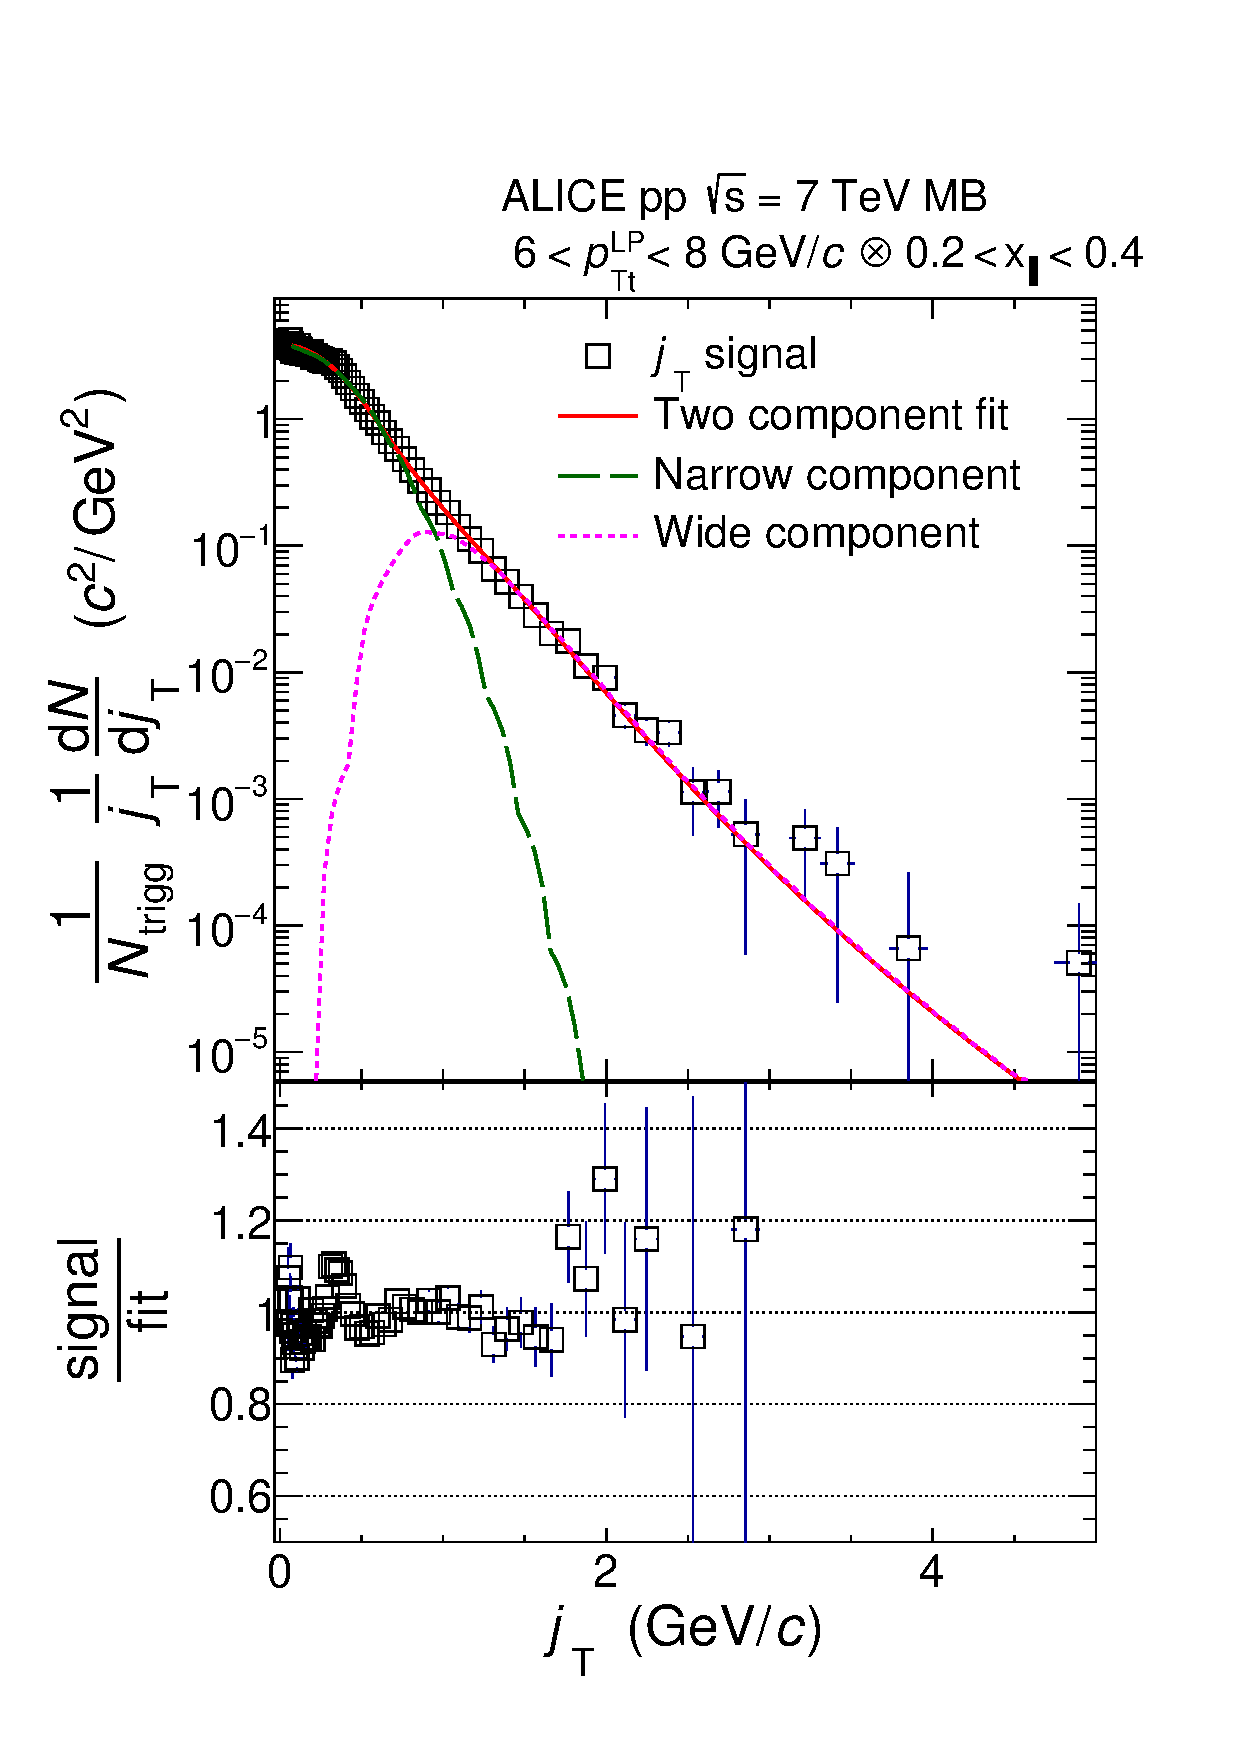
\includegraphics[width = 0.95\textwidth]{pics/jtsignal-89703}
\end{subfigure}
\caption[Dihadron $\jt{}$ results]{\emph{Left:} Measured \jt distribution including a three-component fit. The three components describe the background (circular symbols), hadronization (long dashed line), and showering (short dashed line). \emph{Right:} The same \jt distribution but with background subtracted.}
\label{fig:dihadron}
\end{figure}


%\begin{multline}
%\mathrm{Constant\:\times\:background\:+\:Gauss\:+\:Inverse\:Gamma} \\
%B_0 \times\:\mathrm{background} + \frac{B_2}{B_1\sqrt{2\pi}}e^{-\frac{\jt{}^2}{2B_1^2}}+\frac{B_3B_5^{B_4}}{\Gamma\left(B_4\right)}\frac{e^{-\frac{B_5}{\jt{}}}}{\jt{}^{B_4+1}}.
%\end{multline

The analysis was the first to introduce this factorisation of $\jt{}$ into components.

At $\jt{} \approx 0.4 \gev$ there is a small bump in the distribution to fit ratio. This was attributed to cases where the trigger particle decayed after hadronisation. As it is difficult to correct for, this bump is included in the systematic errors of the results.  


The RMS results from the fitting in both \pp and \pPb collisions are shown in Fig.~\ref{fig:dihadronResults}. Qualitatively the results are similar to jet $\jt{}$ results. The RMS value of the wide component has an increasing trend with respect to $\pt{t}/\pt{jet}$, while the RMS value of the narrow component stays constant. Both components are well described by \pythia~simulations. As seen in the figures there is no difference between \pp and \pPb results in the dihadron analysis. 



\begin{figure}[htb]
\centering
\includegraphics[width=0.95\textwidth]{pics/jt_RMS_finalFormUniformTextSize-89708}
\caption{RMS values of the narrow and wide $\jt{}$ components in the dihadron correlation analysis. Results from \pp collisions at $\sqrt{s} = 7 \tev$ (circular symbols) and from \pPb collisions at \sqrtSnnE{5.02} (square symbols) are compared to \textsc{Pythia}~8 tune 4C simulations at \sqrtSE7 (short dashed line) and at \sqrtSE{5.02} (long dashed line). Different panels correspond to different \xlong bins with 0.2<\xlong<0.4 on the left, 0.4<\xlong<0.6 in the middle, and 0.6<\xlong<1.0 on the right. The statistical errors are represented by bars and the systematic errors by boxes.~\cite{ALICEjt}}
\label{fig:dihadronResults}
\end{figure}


\subsection{Comparing dihadron and jet \texorpdfstring{$\jt{}$}{jT} results}
Comparison to RMS values in dihadron analysis~\cite{ALICEjt} are shown in figure \ref{fig:dihadroncomparison}. For comparison the dihadron trigger $\pt{}$ bins are converted to jet $\pt{}$ bins and vice versa. Bin-by-bin comparison is still not possible, but dihadron analysis gives systematically larger RMS values. This could be caused by several kinematical factors. In jet $\jt{}$ analysis the jet cone limits possible $\jt{}$ values and thus the width and RMS of the $\jt{}$ distributions. The effect of this limitation can be studied by changing the cone size as is described in section \ref{sec:Rstudy}. 

%Comparison to $\jt{}$ results from dihadron analysis ~\cite{ALICEjt} is shown in figure \ref{fig:DihadronComparison}. 
%Trigger $\pt{}$ bins used in dihadron analysis are converted to jet $\pt{}$ bins using observed average jet $\pt{}$ values in leading track momentum bins. Simlarly jet $\pt{}$ bins are converted to $p_{T,\mathrm{trigger}}$ bins using average leading track $\pt{}$ values in $\pt{jet}$ bins.

The trends are similar in dihadron and jet $\jt{}$ results. Wide component RMS values tend to increase with increasing $p_{T,\mathrm{trigger}}$/$\pt{jet}$. Narrow component RMS increases slightly in dihadron analysis but not in jet $\jt{}$, WHY? (Depends on $x_{||}$ bin in dihadron)

In general dihadron $\jt{}$ gives wider distributions with larger RMS values. In jet analysis the cone size limits width and thus the RMS values. The effect of this limitation can be studied by changing the cone size as is described in section \ref{sec:Rstudy}.

Additionally the leading track is an imperfect estimate of the jet/original parton. Because the leading track in general is at an angle compared to the jet axis, the resulting $\jt{}$ values are different. In practice the jet axis found by the jet finding algrorithm tends to minimize the average $\jt{}$ of jet constituents. Thus the yield at high $\jt{}$ is limited and the RMS values are smaller. The effect of having the leading hadron as reference instead of the jet axis is discussed in section ~\ref{sec:reference}

Lastly the results from the dihadron analysis are done in \pt{trigger} bins. This favours hard jets, i.e. jets where the leading hadron carries a large momentum fraction and the jet multiplicity is small. In \pt{jet} bins jets are more likely to be soft, i.e. small leading momentum fraction and high multiplicity jets.



\begin{figure}[htb]
\begin{subfigure}{0.5\textwidth}
\includegraphics[width=0.99\textwidth]{figures/summary/RMSWithSystematics_DihadronTriggerPt.pdf}
\end{subfigure}
\begin{subfigure}{0.5\textwidth}
\includegraphics[width=0.99\textwidth]{figures/summary/RMSWithSystematics_DihadronJetPt.pdf}
\end{subfigure}
\caption{Jet $\jt{}$ results are compared to results obtained in the dihadron analysis. Dihadron trigger $\pt{}$ bins are converted to jet $\pt{}$  bins  using observed mean  $\pt{jet}$ values in $\pt{trigger}$ bins. Dihadron results are for $0.2 < x_{||} < 0.4$}
\label{fig:dihadroncomparison}
\end{figure}

\subsubsection{Different \texorpdfstring{$R$}{R} parameters}
\label{sec:Rstudy}
The size of the jet cone gives a limit for $\jt{}$. For a track with a fixed momentum $p$ this is a hard limit. This is conveniently seen as $\jt{}$ can be given in terms of cone size $R$ and momentum $p$ in the small angle approximation limit as

\begin{equation}
\jt{} \approx p \cdot R
\end{equation}

\noindent  Thus for tracks with $\pt{track} < \pt{0} $, $\jt{} < \pt{0} \times R$.
 

In practice the effect of cone sizes on $\jt{}$ distribution is studied in a \pythia simulation. Results of the individual distributions and resulting RMS values from this simulation are shown in Fig.~\ref{fig:RcomparisonjT} and Fig.~\ref{fig:RcomparisonRMS} respectively. Increasing the cone size of jets gives more room for high $\jt{}$ tracks. This is seen in the individual $\jt{}$ distributions as increased high $\jt{}$ production. At low $\jt{}$ there is no change.

When looking at RMS values from wide component we see an increase/decrease of about 10\% when going from $R=0.4$ to $R=0.5$/$R=0.3$.

The message from narrow component RMS values is less clear. At low jet $\pt{}$ the behaviour is similar, but at high $\pt{}$ the order is reversed.
\begin{figure}[htp]
\centering
\includegraphics[width=0.8\textwidth]{results/RcomparisonSignal.pdf}
\caption[Pythia $R$ parameters $\jt{}$]{Effect of changing $R$ parameter in jet finding on $\jt{}$ distributions}
\label{fig:RcomparisonjT}
\end{figure}


\begin{figure}[htp]
\centering
\includegraphics[width=0.6\textwidth]{figures/results/RcomparisonRMS.pdf} \\
\caption[Pythia $R$ parameters RMS]{Effect of changing $R$ parameter in jet finding on narrow and wide component RMS values. Wide component RMS values increase with increasing cone size.}
\label{fig:RcomparisonRMS}
\end{figure}


%Effect of the $R$ parameter choice is studied in \textsc{Pythia}. Having a fixed cone puts hard limits on the possible $\jt{}$ values. Increasing the cone size loosens these limits and allows higher $\jt{}$ values. The results are shown in Fig. \ref{fig:Rcomparison}. Left hand side shows the $\jt{}$ distributions. There is very little change in low $\jt{}$ but at high $\jt{}$ the yield increases. 

%This is also seen in the RMS values shown in the right hand side of Fig. \ref{fig:Rcomparison}, where the change in wide component RMS is about 10\% when going from $R=0.4$ to $R=0.3$ or $R=0.5$. With the narrow component values the situation is less clear. At low jet $\pt{}$ larger $R$ parameter leads to larger RMS values, but at high $\pt{jet}$ the situation is reversed; increasing the $R$ parameter decreases RMS values.

\subsubsection{Leading tracks versus jet}
\label{sec:reference}
The leading track is an imperfect estimate of the jet/original parton. Because the leading track in general is at an angle compared to the jet axis, the resulting $\jt{}$ values are different. In practice the jet axis found by the jet finding algrorithm tends to minimize the average $\jt{}$ of jet constituents. Thus the yield at high $\jt{}$ is limited and the RMS values are smaller.

A \textsc{Pythia} study was performed where $\jt{}$ was calculated with respect to the leading track momentum, instead of the jet axis. The results are shown in Fig. \ref{fig:RefComparison}. The resulting $\jt{}$ distributions are significantly wider than $\jt{}$ distributions from the typical method. The effect seems to be larger than the effect seen in comparing different $R$ values.

\begin{figure}[htp]
\centering
\includegraphics[width=0.55\textwidth]{figures/results/JetVsLeadingRefConst.pdf}
\caption{Results of calculating $\jt{}$ with respect to the jet axis or the leading hadron. The assumption is that because the leading hadron is an imperfect estimate of the jet axis, low $\jt{}$ tracks should on average be shifted to higher $\jt{}$}
\label{fig:RefComparison}
\end{figure}


\pagebreak
\FloatBarrier
\section{Summary}
\label{sec:sum}
In this work two distinct $\jt{}$ components were extracted for narrow and wide contributions using jet reconstruction in $\snn = \unit[5.02]{\tev}$ \pPb collisions. RMS values for both components were obtained. The width of the wide component is found to increase for increasing $\pt{jet}$. This is in part explained by the changing kinematical limits when going to higher $\pt{jet}$ which allows higher $\pt{track}$. Additionally the larger phase space allows stronger parton splitting. The results are qualitatively compatible with previous studies that studied $\jt{}$ using two-particle correlations.

{\color{red} Extend summary}


%\appendix
%\addtocontents{toc}{\protect\contentsline{section}{Appendix:}}
%\include{AppendixA}

%\include{AppendixA}


\bibliographystyle{h-physrev3}
%\bibliographystyle{prsty}
%\bibliographystyle{h-elsevier}

\bibliography{mastercites, biblio}


\end{document}  


